\section{安定化制御実験}
	振子を上向きに配置したときに安定化制御が可能か実験を行う(実験目的の第一項目)。
	その際に、振子を真上に配置するのではなく、十数度角度をつけてから実験を始める。
	実験に用いたパラメータを以下の表に示す。
	\begin{table}[H]
		\begin{center}
			\caption{安定化制御実験で使用したパラメータの組}
			\medskip
			
			\begin{tabular}{|c|c|c|c|}\hline
				重み行列$Q$ & オブザーバの極$P$ & サンプリング周期$\Delta[\rm{s}]$ \\ \hline\hline
				$Q_1$:$\rm{diag}(1E5,1E5,1,1)$ & $P_1$:$((-30,0),(-30,0))^{'}$ & $\Delta_1$:0.005 \\ \hline
			\end{tabular}
		\end{center}
		\label{table:huriage_control}
	\end{table}
	以下に実験結果とシミュレーション結果の比較した図を示す。
	\begin{figure}[H]
		\centering
		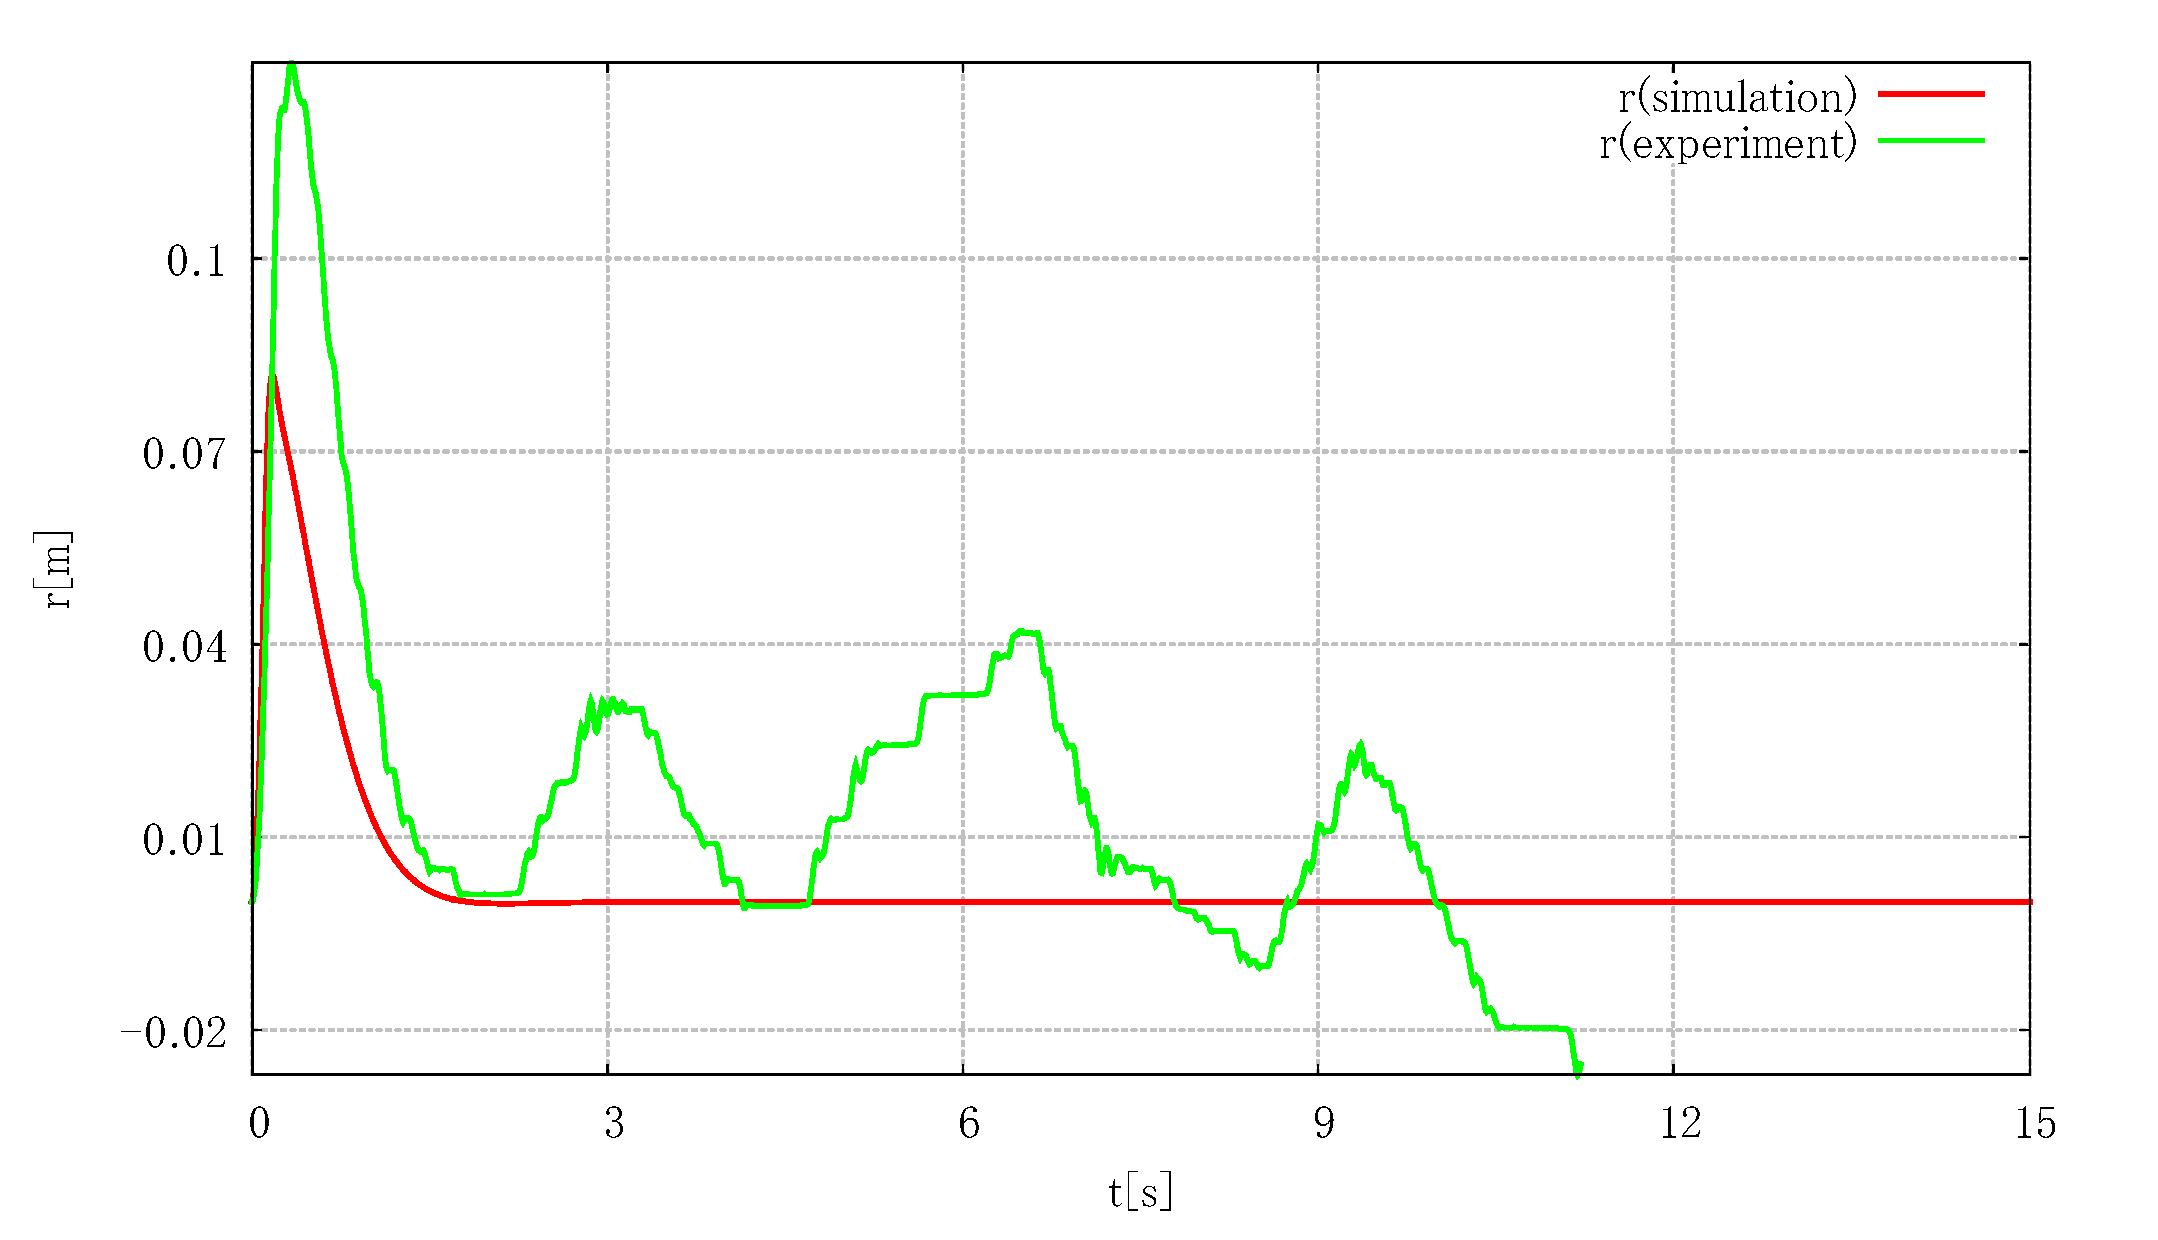
\includegraphics[width=0.8\linewidth]{gazo/experiment_control_R.eps}
		\caption{安定化制御実験結果(台車位置)}
		\label{image:experiment_control_R}
	\end{figure}
	\begin{figure}[H]
		\centering
		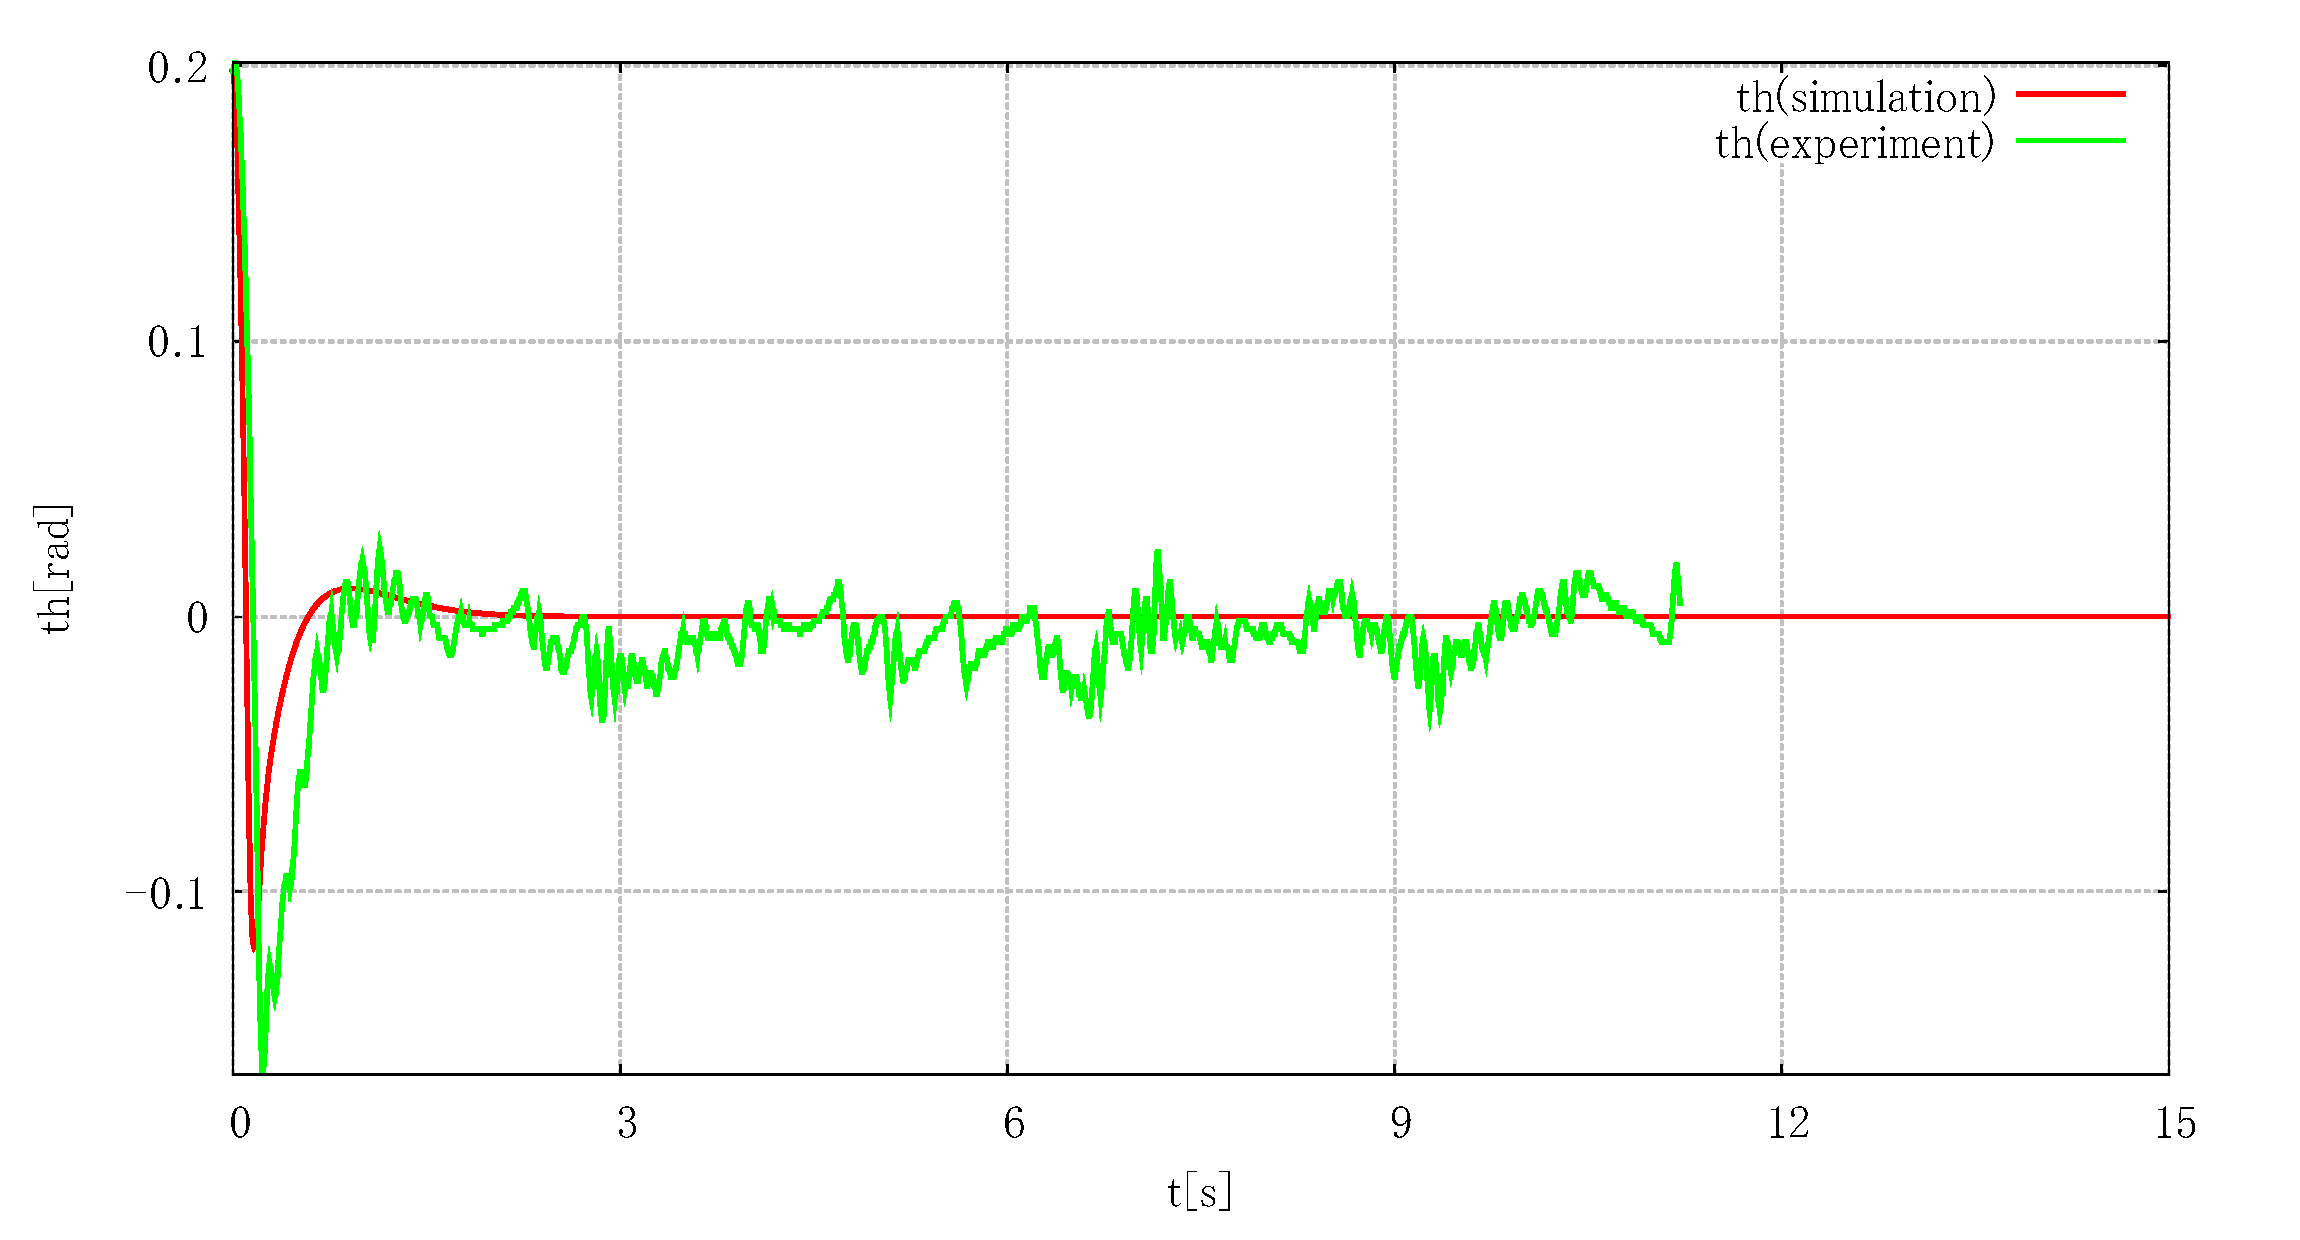
\includegraphics[width=0.8\linewidth]{gazo/experiment_control_TH.eps}
		\caption{安定化制御実験結果(振子角度)}
		\label{image:experiment_control_TH}
	\end{figure}
	図\ref{image:experiment_control_R}と図\ref{image:experiment_control_TH}
	より一番最初の山は実験のほうが大幅に大きくなっていることと、ノイズが乗っている点を除いてシミュレーションと実験結果は
	概ね一致しているといえる。これは、実験のほうではデータの計測を開始して振子から手を離したためその影響が出たといえる。
	この時の初期角度は$11.34°$である。
	よって、初期角度が十数度ある中で実験を開始し、安定化制御を行うことができたため、
	実験目的の第一項目を達成できたといえる。
	
	
	
%-----------------------------------------------------------
\newpage
\section{目標値の変更実験}
	台車に目標値を与えて、その目標値に台車が移動しても安定化制御可能か実験を行う(実験項目の第二項目)。
	なお、目標値は5秒ごとに0→0.1→0のように変更される。
	以下に、重み行列を変更した場合の比較、オブザーバの極を変更した場合の比較、サンプリング周期を変更した場合の比較を
	行った図を示す。
	\par
	%-----------------------------------------------------------------------------------
	\subsection{重み行列の違いによる実験結果の比較}
	最初に重み行列を変更した場合の実験結果の比較を見てみる。
	\begin{figure}[H]
		\centering
		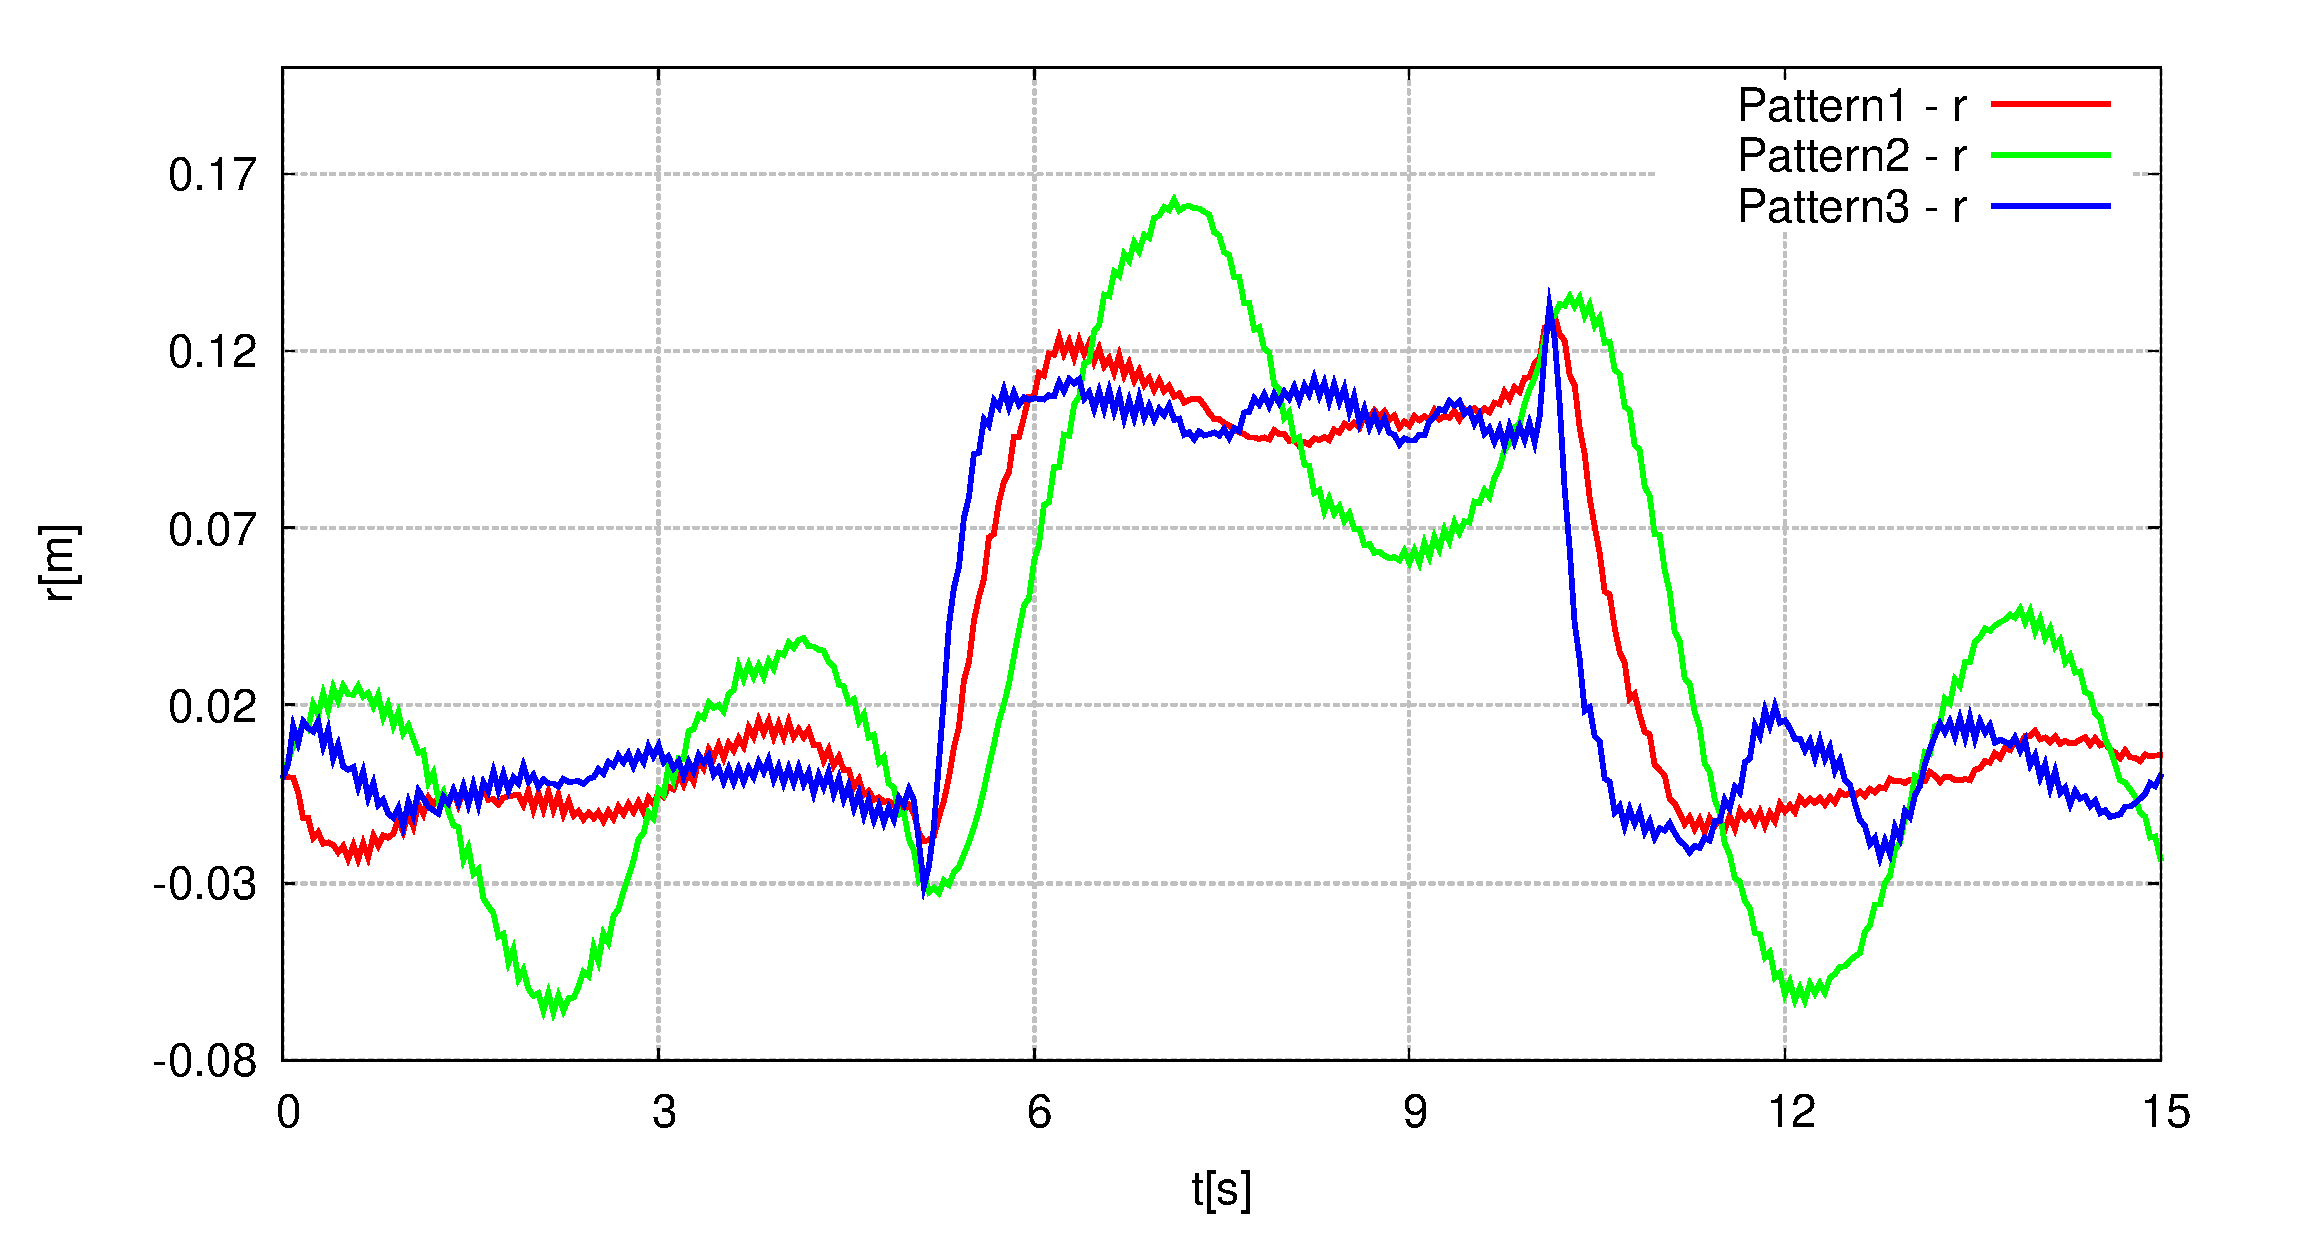
\includegraphics[width=0.49\linewidth]{gazo/Compare_Q_R2.eps}
		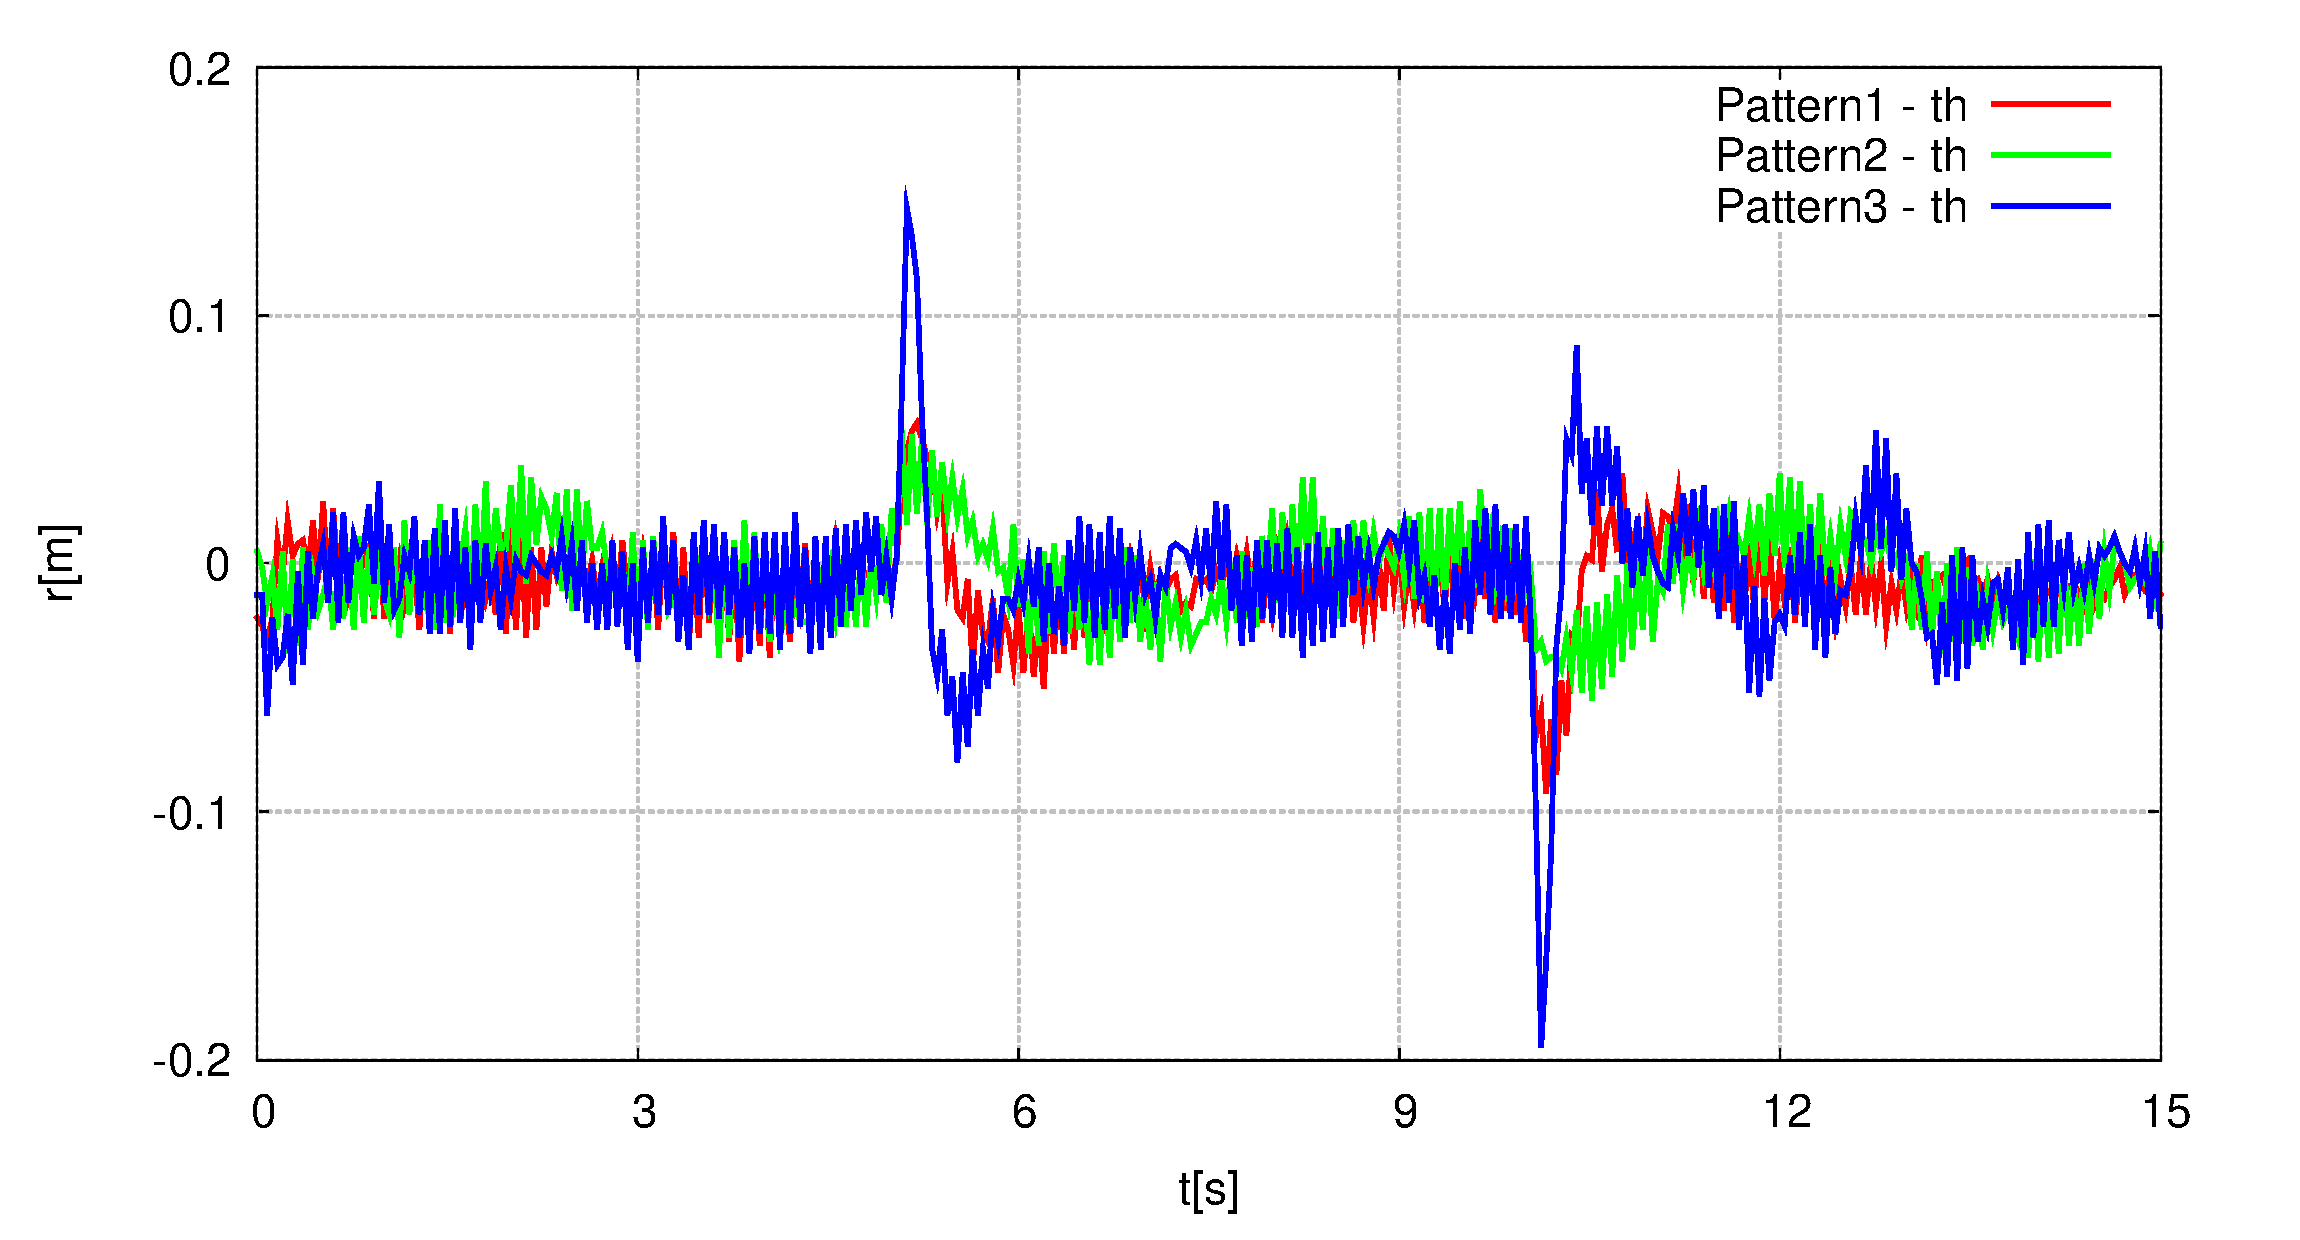
\includegraphics[width=0.49\linewidth]{gazo/Compare_Q_TH2.eps}
		\caption{重み行列の違いによる実験結果の比較}
		\label{image:comp_Q}
	\end{figure}
	図中のPatternは以下の表に対応するパラメータである。
	\begin{table}[H]
		\begin{center}
			\caption{パターンとパラメータの対応表}
			\medskip
			
			\begin{tabular}{|c|c|c|c|}\hline
				パターン & 重み行列$Q$ & オブザーバの極$P$ & サンプリング周期$\Delta[\rm{s}]$ \\ \hline\hline
				Pattern1 & $Q_1$:$\rm{diag}(1E5,1E5,1,1)$ & $P_1$:$((-30,0),(-30,0))^{'}$ & $\Delta_1$:0.005 \\ \hline
				Pattern2 & $Q_1$:$\rm{diag}(1E5,1E6,1,1)$ & $P_1$:$((-30,0),(-30,0))^{'}$ & $\Delta_1$:0.005 \\ \hline
				Pattern3 & $Q_1$:$\rm{diag}(1E6,1E5,1,1)$ & $P_1$:$((-30,0),(-30,0))^{'}$ & $\Delta_1$:0.005 \\ \hline
			\end{tabular}
		\end{center}
		\label{table:huriage_control}
	\end{table}
	図\ref{image:comp_Q}の左図を見えると、台車の位置に関しては、パターン3→パターン1→パターン2の順に応答が遅くなっていることがわかる。
	特にパターン2の方は目標値変更に対して台車が移動してはいるが、波打って動いていることがわかる。つまり、
	重み行列の第一成分を大きくしているパターン3の応答が一番よく、重み行列の第二成分を大きくしたパターン2
	はバランスがくずれてしまい応答が一番悪いといえる。
	右図の振子の角度についても同様のことが言える。パターン3は台車が動く時に角度が大きく傾いてしまっているが、パターン2は台車が動く時においても、大きな角度の傾きは確認できない。
	つまり、重み行列の第二成分を大きくしているパターン2の応答が一番よく、重み行列の第一成分を大きくしたパターン3は
	バランスが崩れてしまい応答が一番悪いといえる。
	シミュレーションの章でも述べたように重み行列の各成分は各状態に対応しており、応答を良くしたい状態があれば、それに対応する
	成分をおおきくすればよいということが実験でも確認できる。
	\par
	%--------------------------------------------------------------------------------------------------------
	\subsection{オブザーバの極の違いによる実験結果の比較}
	次にオブザーバの極の違いによる実験結果の比較を見てみる。
	\begin{figure}[H]
		\centering
		\includegraphics[width=0.49\linewidth]{gazo/Compare_obs_R2.eps}
		\includegraphics[width=0.49\linewidth]{gazo/Compare_obs_TH2.eps}
		\caption{オブザーバの極の違いによる実験結果の比較}
		\label{image:comp_obs}
	\end{figure}
	図中のPatternは以下の表に対応するパラメータである。
	\begin{table}[H]
		\begin{center}
			\caption{パターンとパラメータの対応表}
			\medskip
			
			\begin{tabular}{|c|c|c|c|}\hline
				パターン & 重み行列$Q$ & オブザーバの極$P$ & サンプリング周期$\Delta[\rm{s}]$ \\ \hline\hline
				Pattern1 & $Q_1$:$\rm{diag}(1E5,1E5,1,1)$ & $P_1$:$((-30,0),(-30,0))^{'}$ & $\Delta_1$:0.005 \\ \hline
				Pattern2 & $Q_1$:$\rm{diag}(1E5,1E5,1,1)$ & $P_1$:$((-60,0),(-60,0))^{'}$ & $\Delta_1$:0.005 \\ \hline
			\end{tabular}
		\end{center}
		\label{table:huriage_control}
	\end{table}
	図\ref{image:comp_obs}の左図より、台車の位置についてはパターン1とパターン2において応答の速さで大きな違いはないといえる。
	しかし、台車の位置が0.1になったときのパターン2の波形はパターン1の波形と比べて振動的になっていいることがわかる。このことから、
	オブザーバーの極が虚軸から遠くなると応答は振動的になると考えられる。
	右図より、振子の角度については、パターン1とパターン2では大きな違いは確認できないといえる。
	\newpage
	%--------------------------------------------------------------------------------------------------
	\subsection{サンプリング周期の違いによる実験結果の比較}
	次にサンプリング周期の違いによる実験結果の比較を見てみる。
	\begin{figure}[H]
		\centering
		\includegraphics[width=0.49\linewidth]{gazo/Compare_dt_R2.eps}
		\includegraphics[width=0.49\linewidth]{gazo/Compare_dt_TH2.eps}
		\caption{サンプリング周期の違いによる実験結果の比較}
		\label{image:comp_dt}
	\end{figure}
	図中のPatternは以下の表に対応するパラメータである。
	\begin{table}[H]
		\begin{center}
			\caption{パターンとパラメータの対応表}
			\medskip
			
			\begin{tabular}{|c|c|c|c|}\hline
				パターン & 重み行列$Q$ & オブザーバの極$P$ & サンプリング周期$\Delta[\rm{s}]$ \\ \hline\hline
				Pattern1 & $Q_1$:$\rm{diag}(1E5,1E5,1,1)$ & $P_1$:$((-30,0),(-30,0))^{'}$ & $\Delta_1$:0.005 \\ \hline
				Pattern2 & $Q_1$:$\rm{diag}(1E5,1E5,1,1)$ & $P_1$:$((-30,0),(-30,0))^{'}$ & $\Delta_1$:0.010 \\ \hline
			\end{tabular}
		\end{center}
		\label{table:huriage_control}
	\end{table}
	図\ref{image:comp_dt}の左図より、台車の位置についてはサンプリング周期が長い方のパターン2の方が0.1に移動した際の台車の位置と0に移動する直前の台車の位置に大きな
	ズレがないことがわかる。これはサンプリング周期が長いため台車の動きが緩やかになったためと考える。右図より、振子の角度については
	目標値が0に戻る時点での角度のズレがパターン2の方が小さいことがわかる。台車の位置が大きくズレなかった結果、振子の角度のズレも小さくなったといえるが、
	サンプリング周期が長い影響であるともいえる。つまり、サンプリング周期が長くなったことで、拾いきれない情報が存在し、台車の動きが緩やかになったといえる。
	\newpage
	%---------------------------------------------------------------------------------------------------------
	\subsection{シミュレーション結果と実験結果の比較}
	以下に実験結果とシミュレーション結果との比較を行った図を示す。
	また、図の数が多いので図のキャプションとその図における各パラメータの対応表を示す。
	\begin{table}[H]
		\begin{center}
			\caption{図に対応するパラメータの組}
			\begin{tabular}{|c|c|c|c|}\hline
				図のキャプション & 重み行列$Q$ & オブザーバの極$P$ & サンプリング周期$\Delta[\rm{s}]$ \\ \hline\hline
				比較結果その1 & $Q_1$:$\rm{diag}(1E5,1E5,1,1)$ & $P_1$:$((-30,0),(-30,0))^{'}$ & $\Delta_1$:0.005 \\ \hline
				比較結果その2 & $Q_1$:$\rm{diag}(1E5,1E6,1,1)$ & $P_1$:$((-30,0),(-30,0))^{'}$ & $\Delta_1$:0.005 \\ \hline
				比較結果その3 & $Q_1$:$\rm{diag}(1E6,1E5,1,1)$ & $P_1$:$((-30,0),(-30,0))^{'}$ & $\Delta_1$:0.005 \\ \hline
				比較結果その4 & $Q_1$:$\rm{diag}(1E5,1E5,1,1)$ & $P_1$:$((-60,0),(-60,0))^{'}$ & $\Delta_1$:0.005 \\ \hline
				比較結果その5 & $Q_1$:$\rm{diag}(1E5,1E6,1,1)$ & $P_1$:$((-60,0),(-60,0))^{'}$ & $\Delta_1$:0.005 \\ \hline
				比較結果その6 & $Q_1$:$\rm{diag}(1E6,1E5,1,1)$ & $P_1$:$((-60,0),(-60,0))^{'}$ & $\Delta_1$:0.005 \\ \hline
				比較結果その7 & $Q_1$:$\rm{diag}(1E5,1E5,1,1)$ & $P_1$:$((-30,0),(-30,0))^{'}$ & $\Delta_1$:0.010 \\ \hline
				比較結果その8 & $Q_1$:$\rm{diag}(1E5,1E6,1,1)$ & $P_1$:$((-30,0),(-30,0))^{'}$ & $\Delta_1$:0.010 \\ \hline
				比較結果その9 & $Q_1$:$\rm{diag}(1E6,1E5,1,1)$ & $P_1$:$((-30,0),(-30,0))^{'}$ & $\Delta_1$:0.010 \\ \hline
				比較結果その10 & $Q_1$:$\rm{diag}(1E5,1E5,1,1)$ & $P_1$:$((-60,0),(-60,0))^{'}$ & $\Delta_1$:0.010 \\ \hline
				比較結果その11 & $Q_1$:$\rm{diag}(1E5,1E6,1,1)$ & $P_1$:$((-60,0),(-60,0))^{'}$ & $\Delta_1$:0.010 \\ \hline
				比較結果その12 & $Q_1$:$\rm{diag}(1E6,1E5,1,1)$ & $P_1$:$((-60,0),(-60,0))^{'}$ & $\Delta_1$:0.010 \\ \hline
			\end{tabular}
		\end{center}
		\label{table:huriage_control}
	\end{table}
	
	\begin{figure}[H]
		\centering
		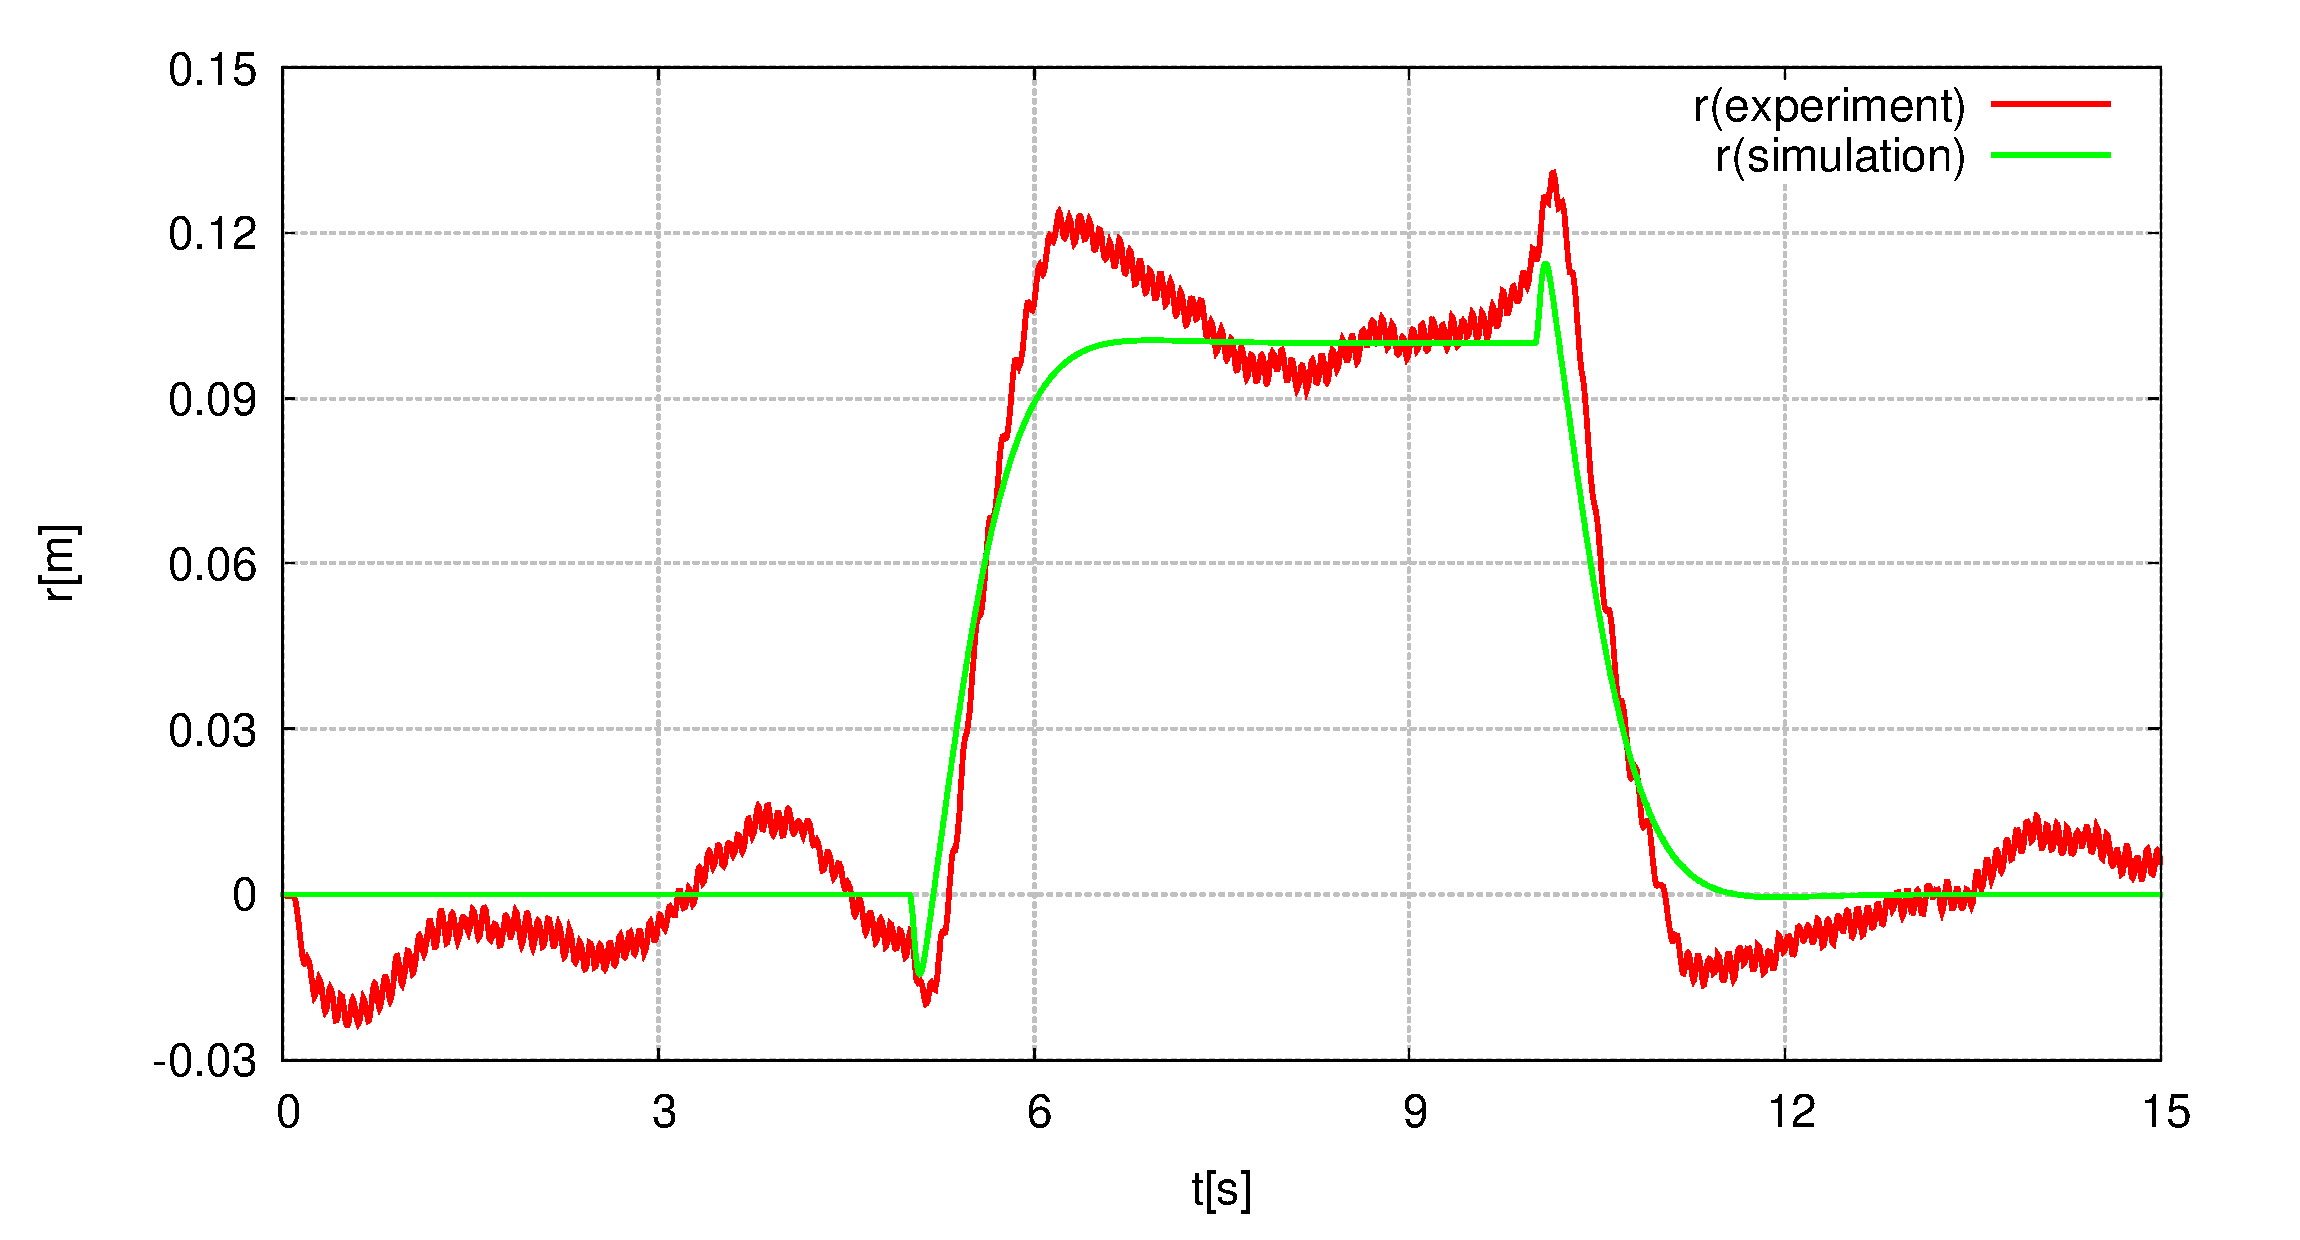
\includegraphics[width=0.49\linewidth]{gazo/experiment_Q55obs30dt05R2.eps}
		\includegraphics[width=0.49\linewidth]{gazo/experiment_Q55obs30dt05TH2.eps}
		\caption{比較結果その1(左図がr,右図が$\theta$)}
		\label{image:sono1}
	\end{figure}
	\begin{figure}[H]
		\centering
		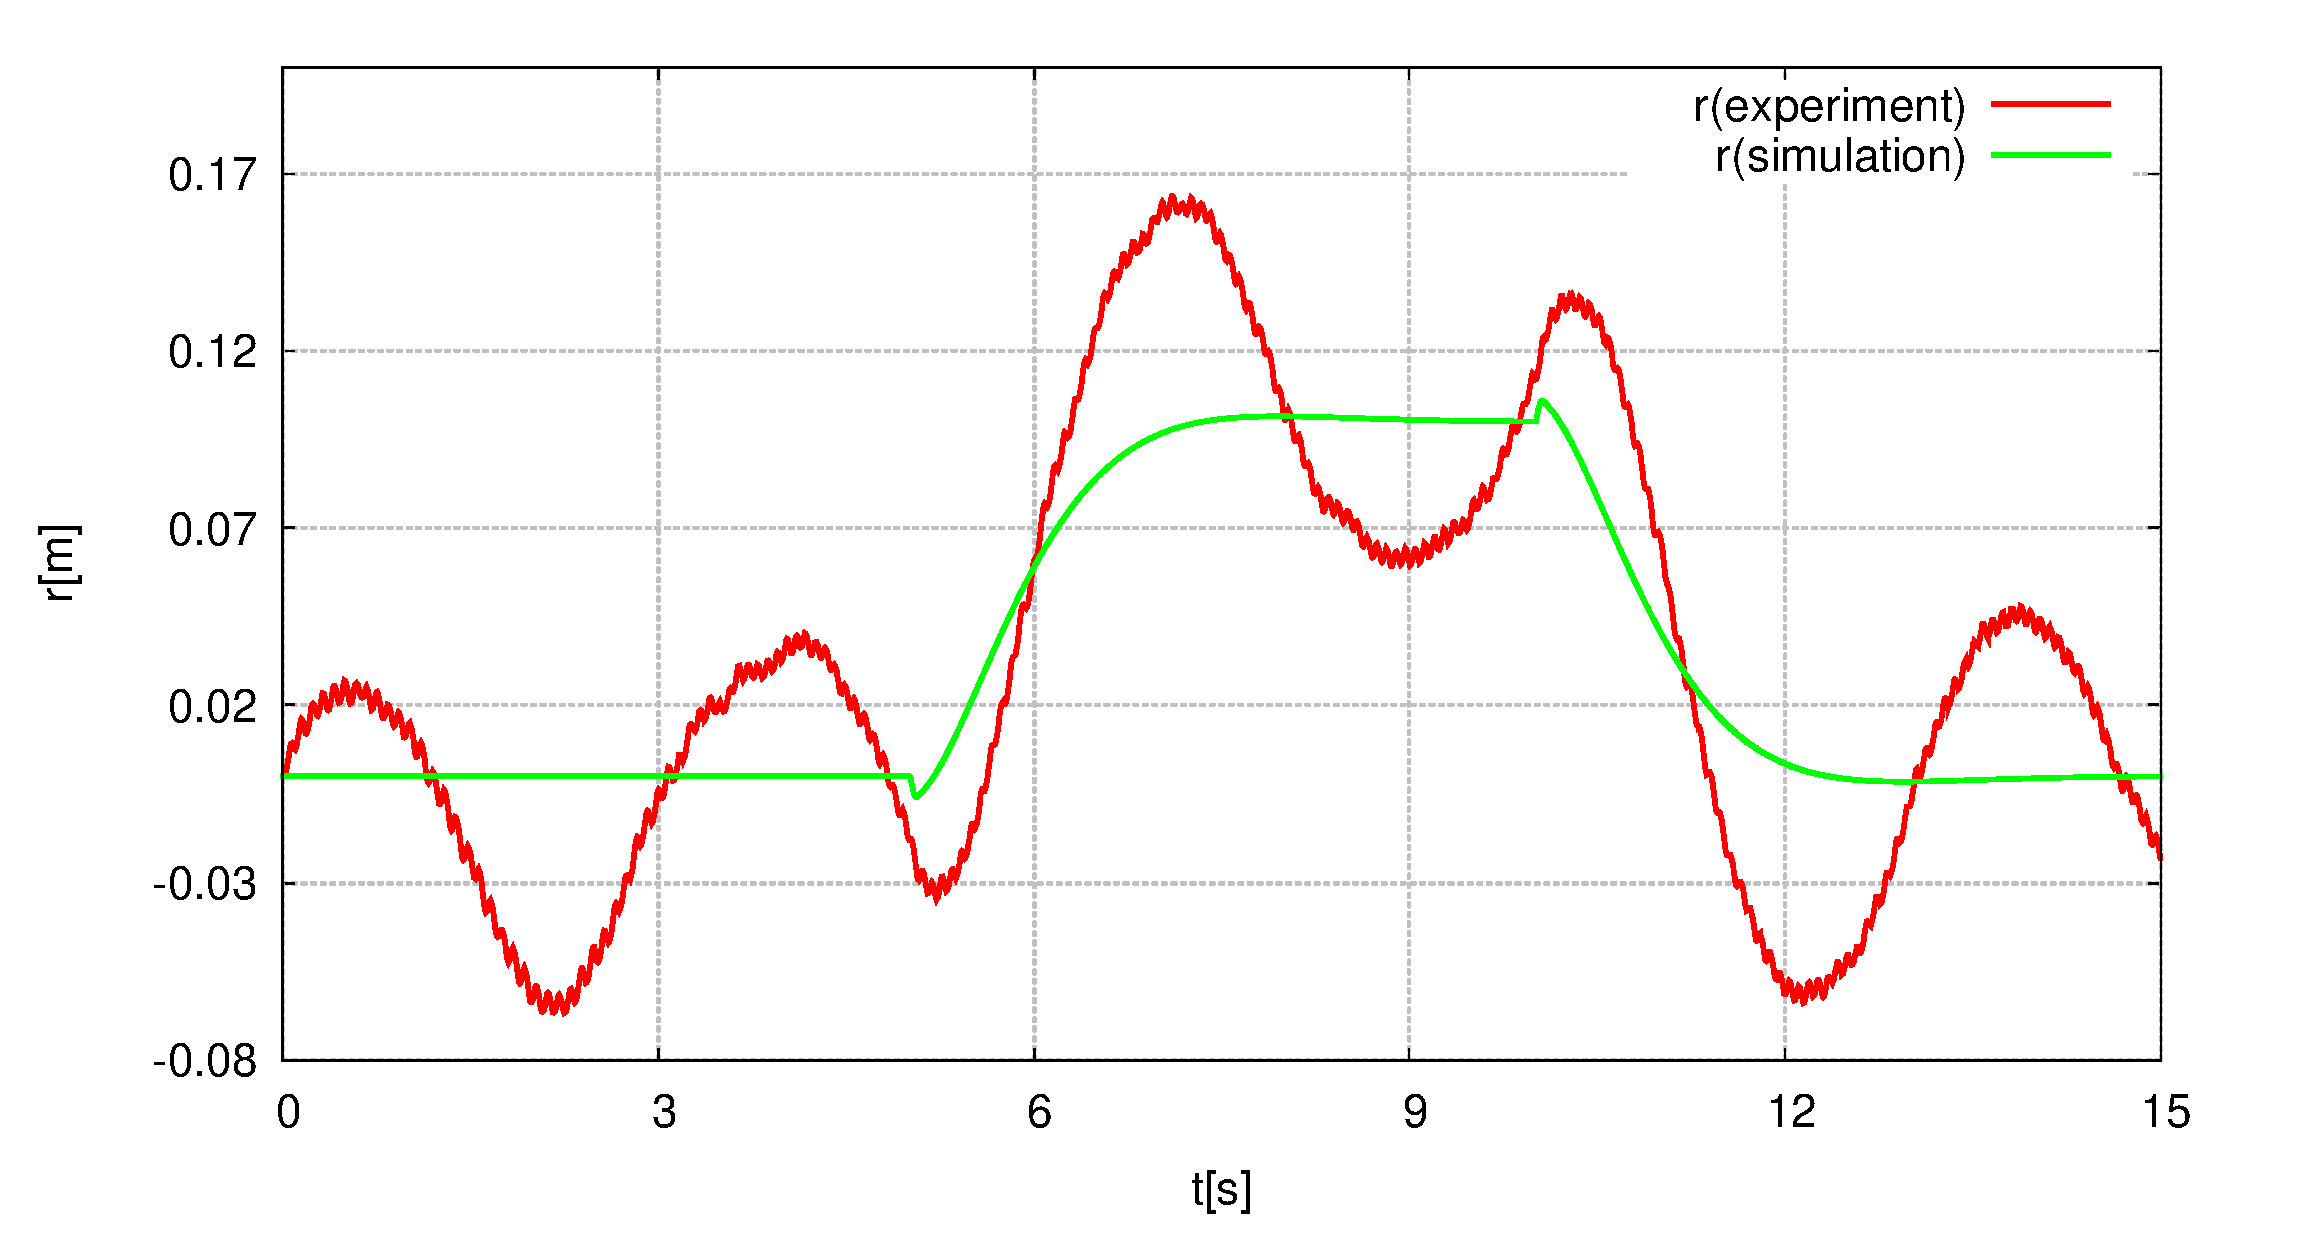
\includegraphics[width=0.49\linewidth]{gazo/experiment_Q56obs30dt05R2.eps}
		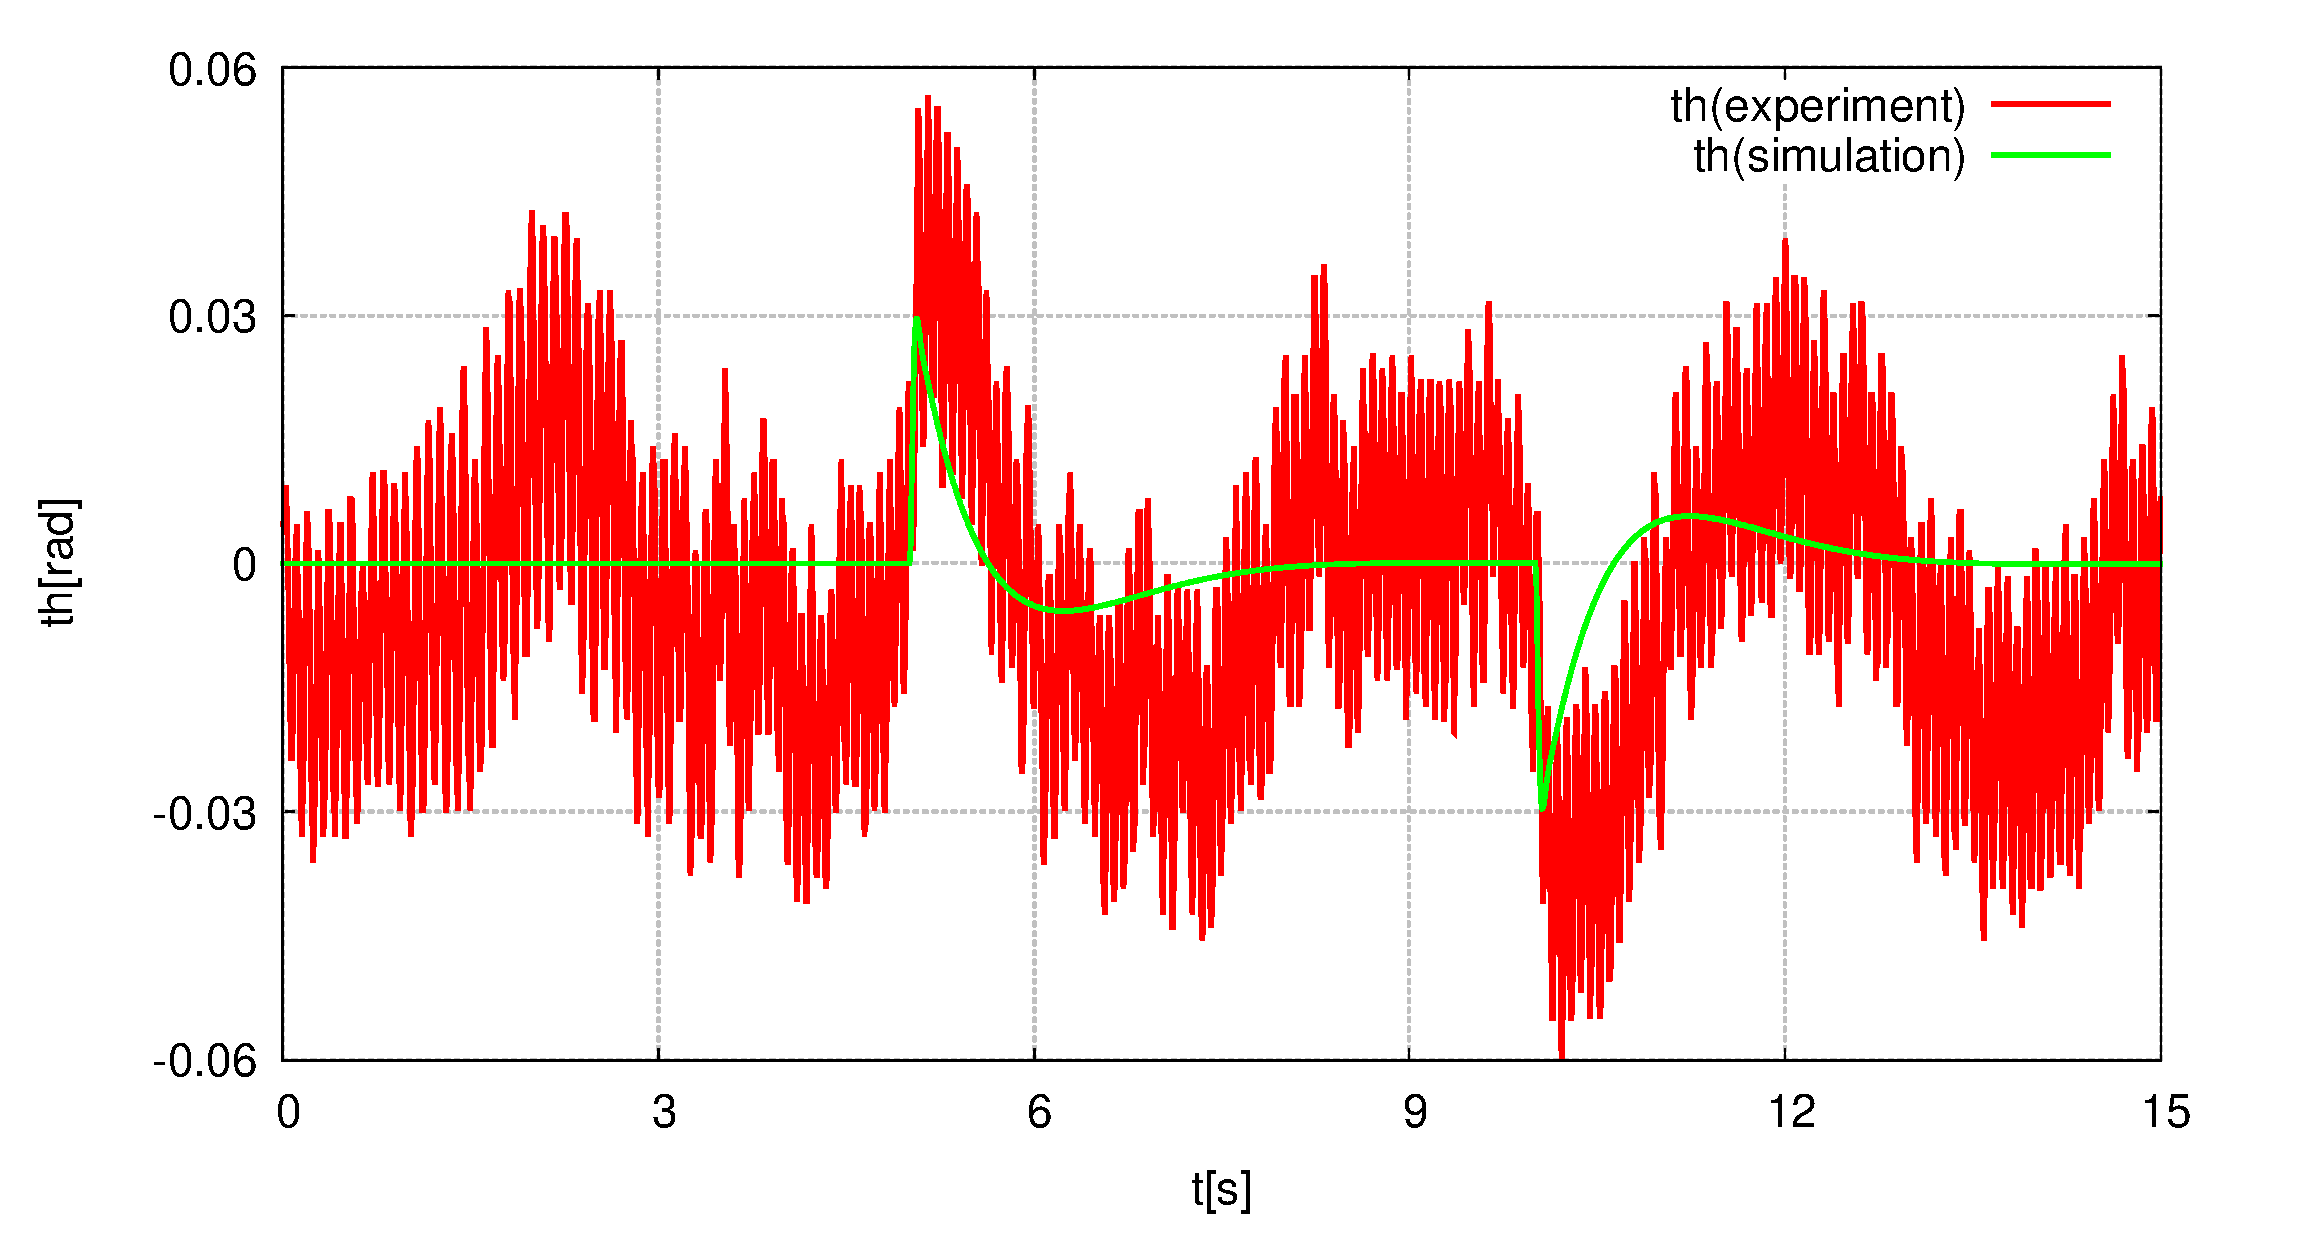
\includegraphics[width=0.49\linewidth]{gazo/experiment_Q56obs30dt05TH2.eps}
		\caption{比較結果その2(左図がr,右図が$\theta$)}
		\label{image:sono2}
	\end{figure}
	\begin{figure}[H]
		\centering
		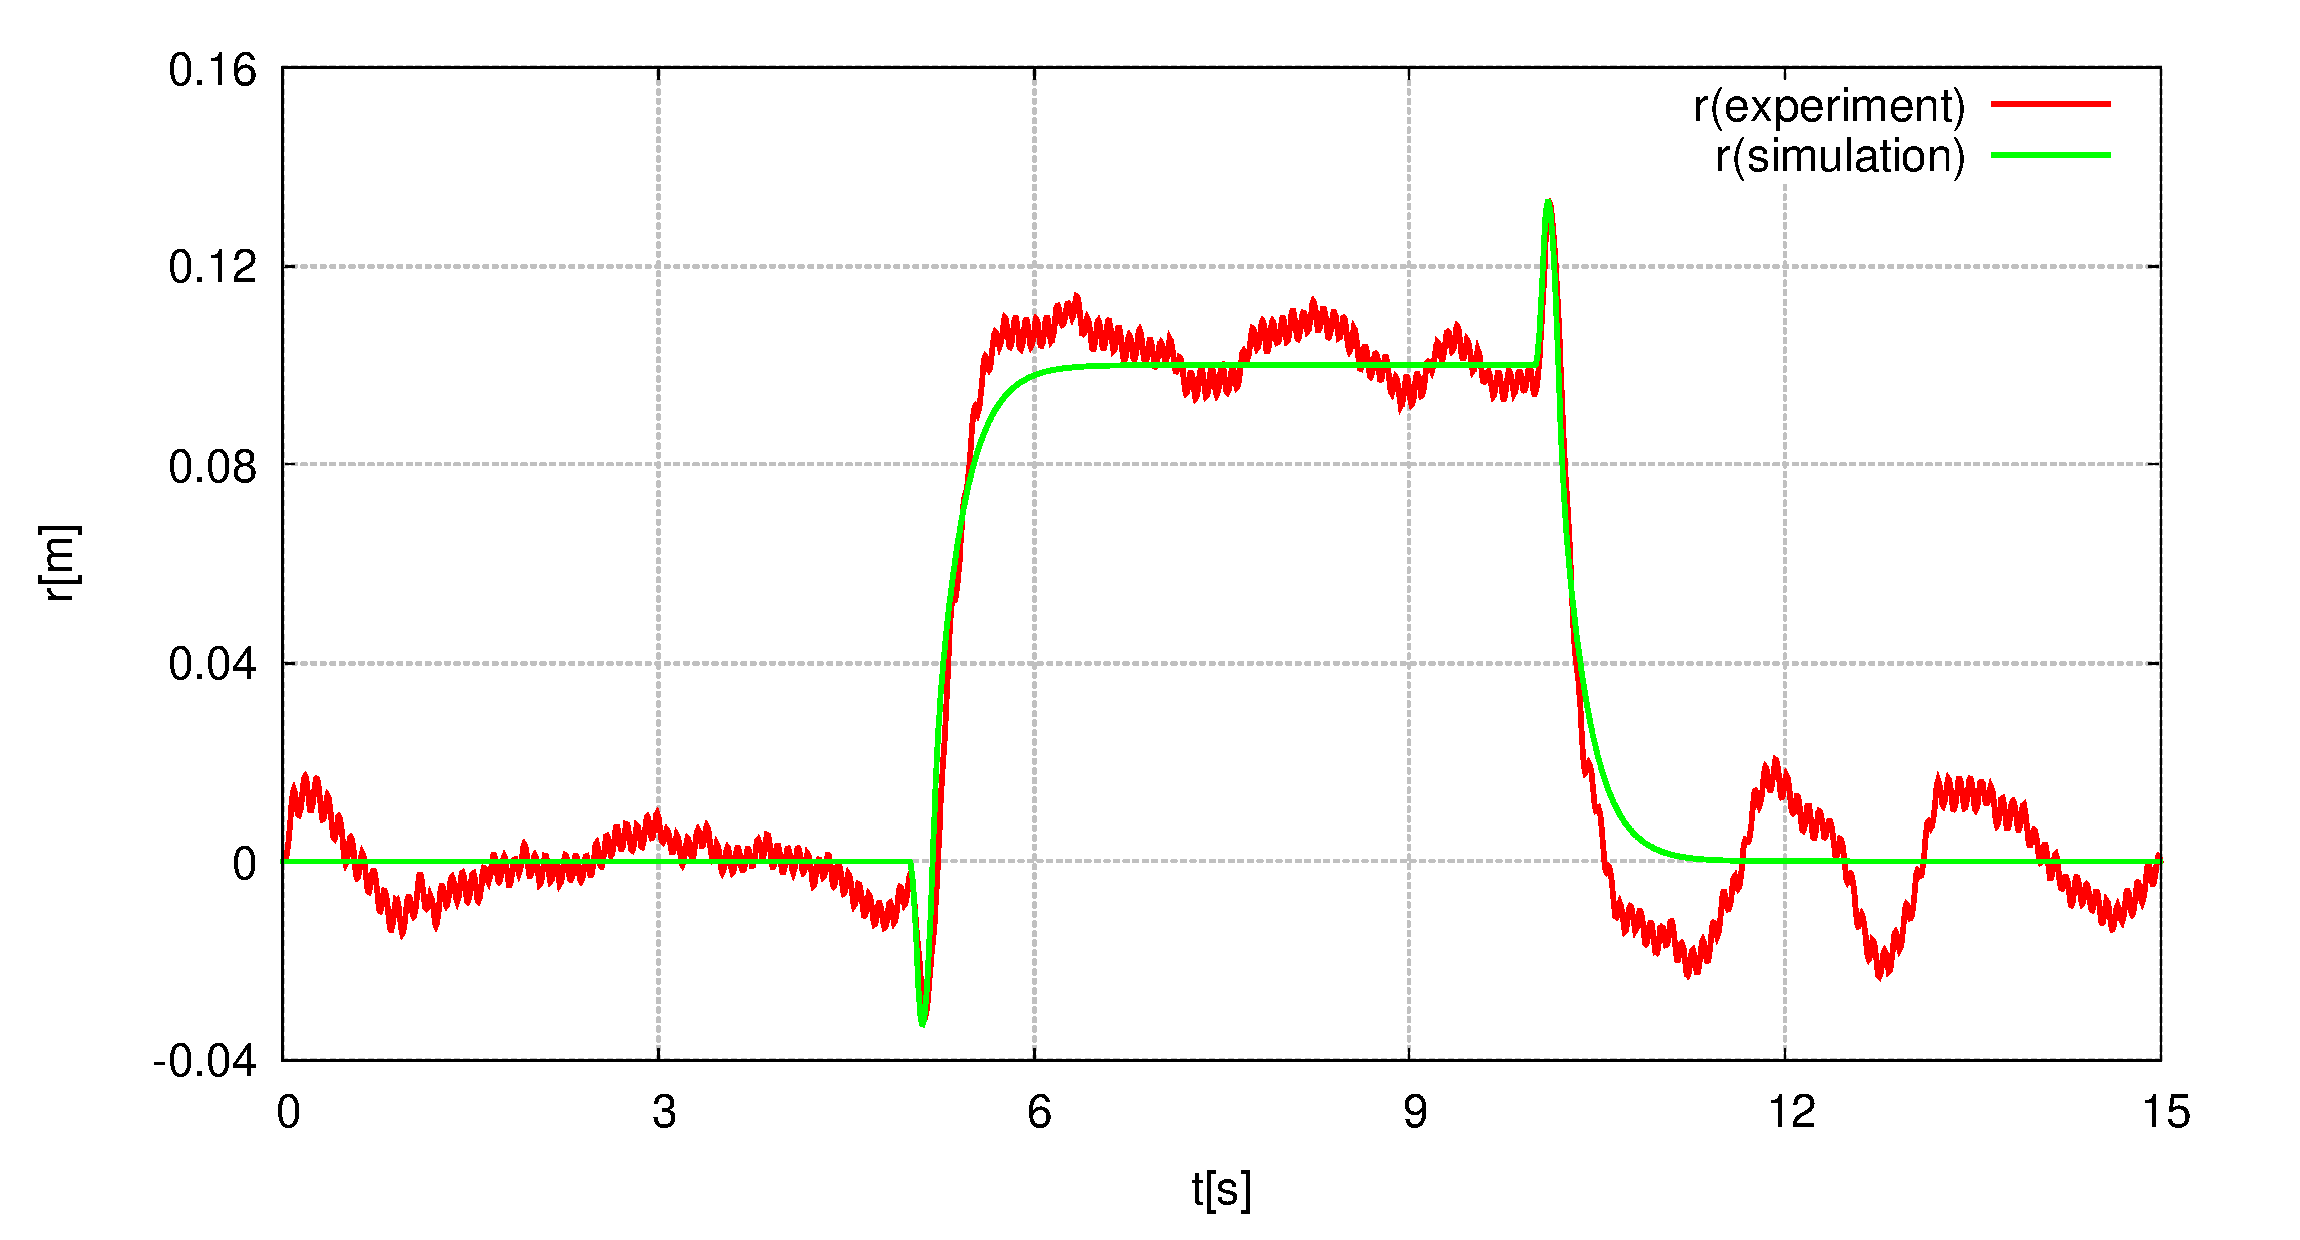
\includegraphics[width=0.49\linewidth]{gazo/experiment_Q65obs30dt05R2.eps}
		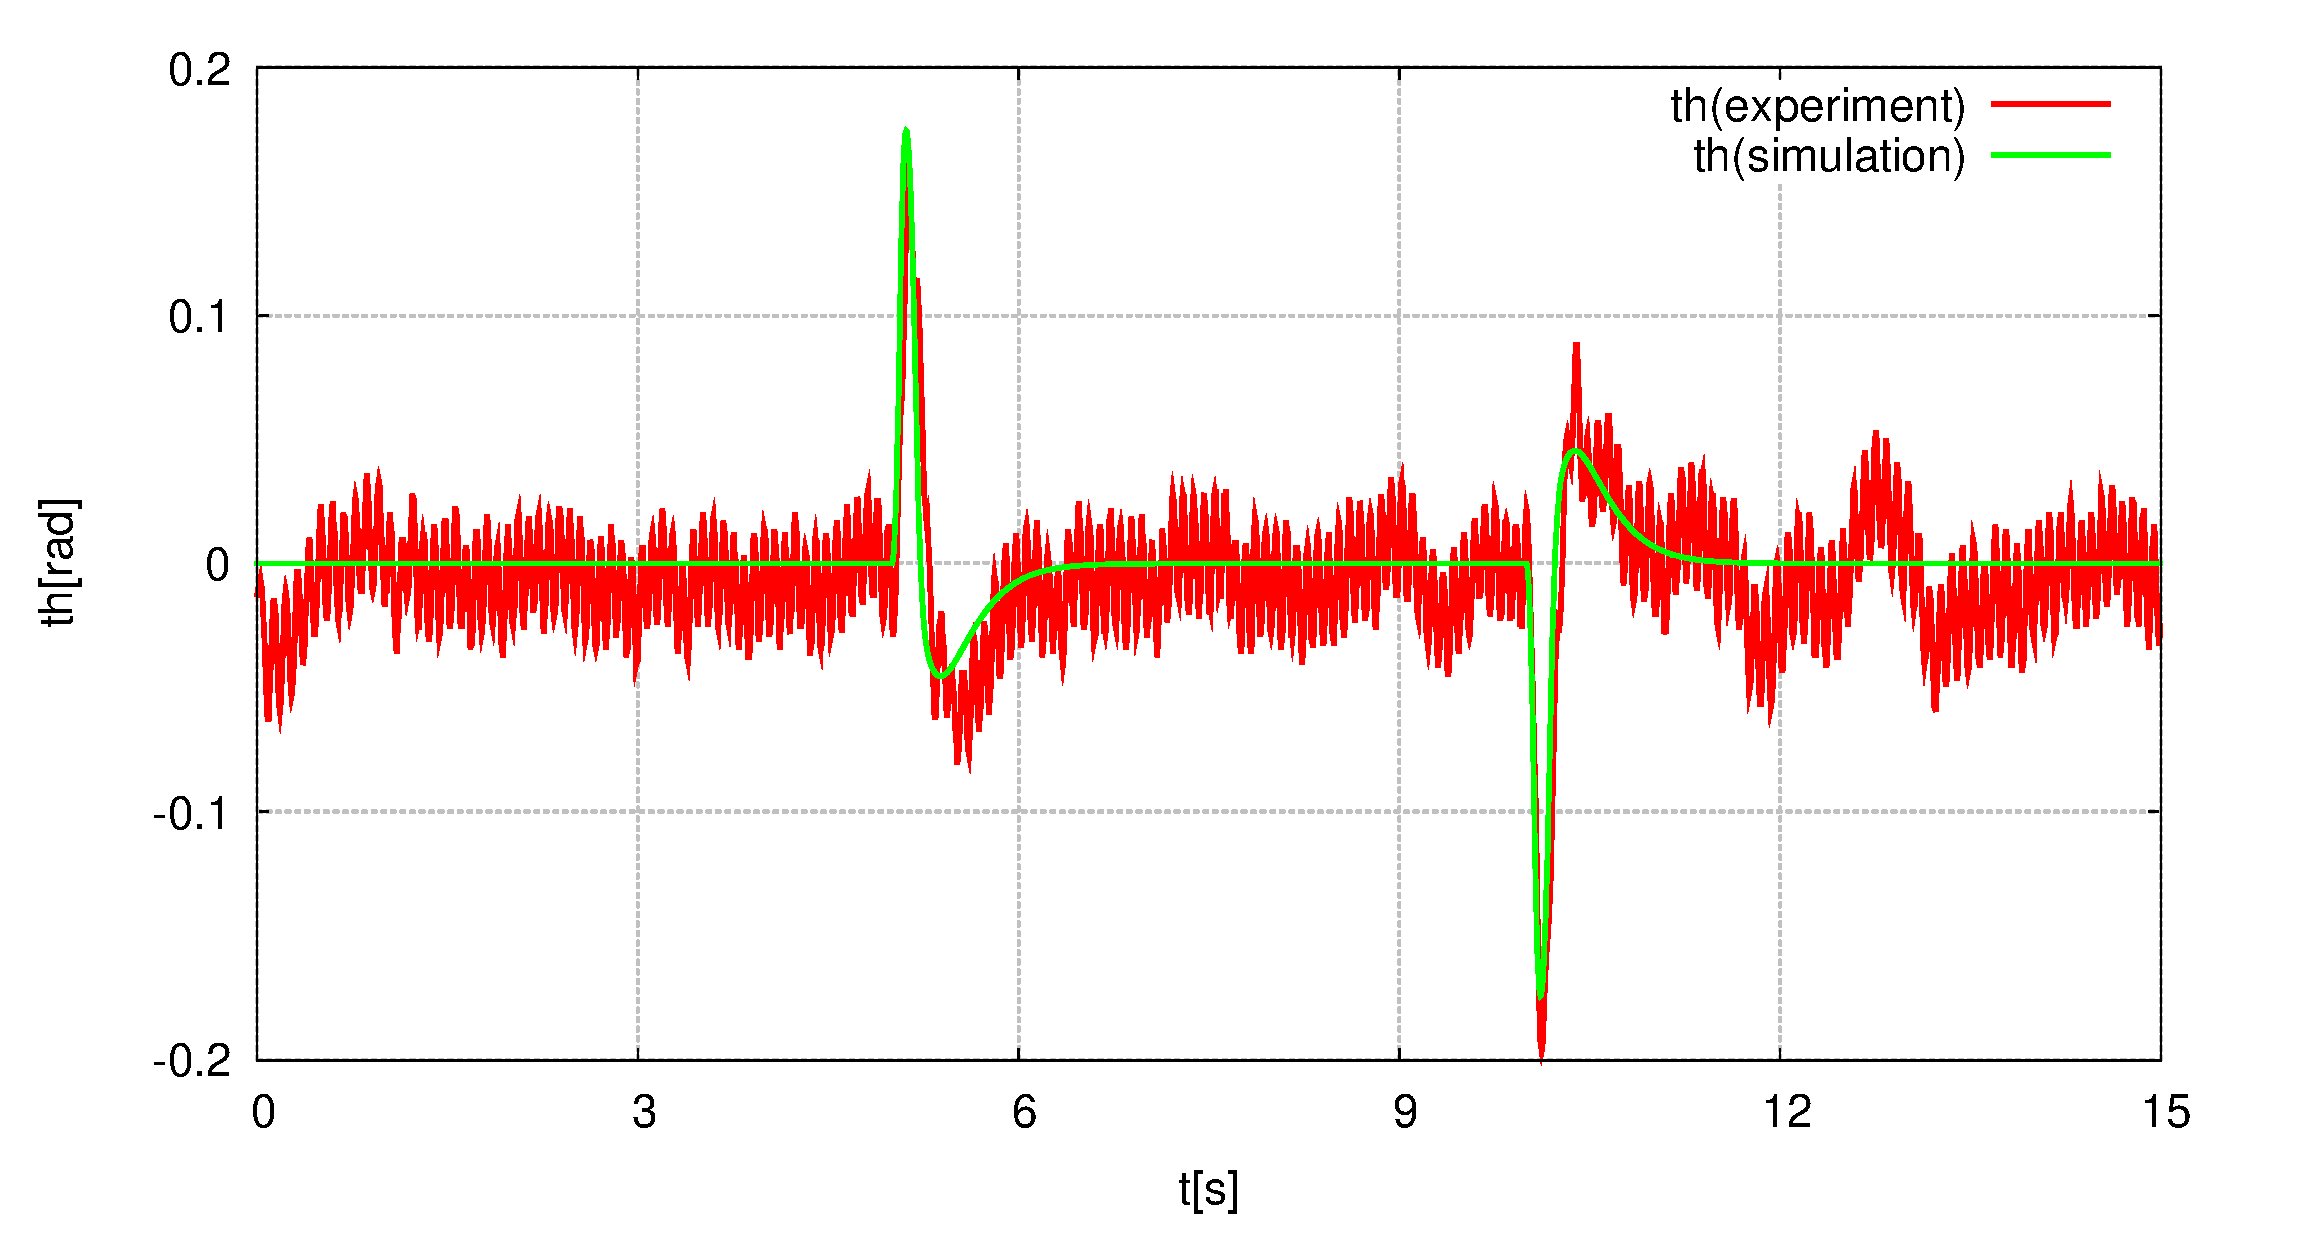
\includegraphics[width=0.49\linewidth]{gazo/experiment_Q65obs30dt05TH2.eps}
		\caption{比較結果その3(左図がr,右図が$\theta$)}
		\label{image:sono3}
	\end{figure}
	\begin{figure}[H]
		\centering
		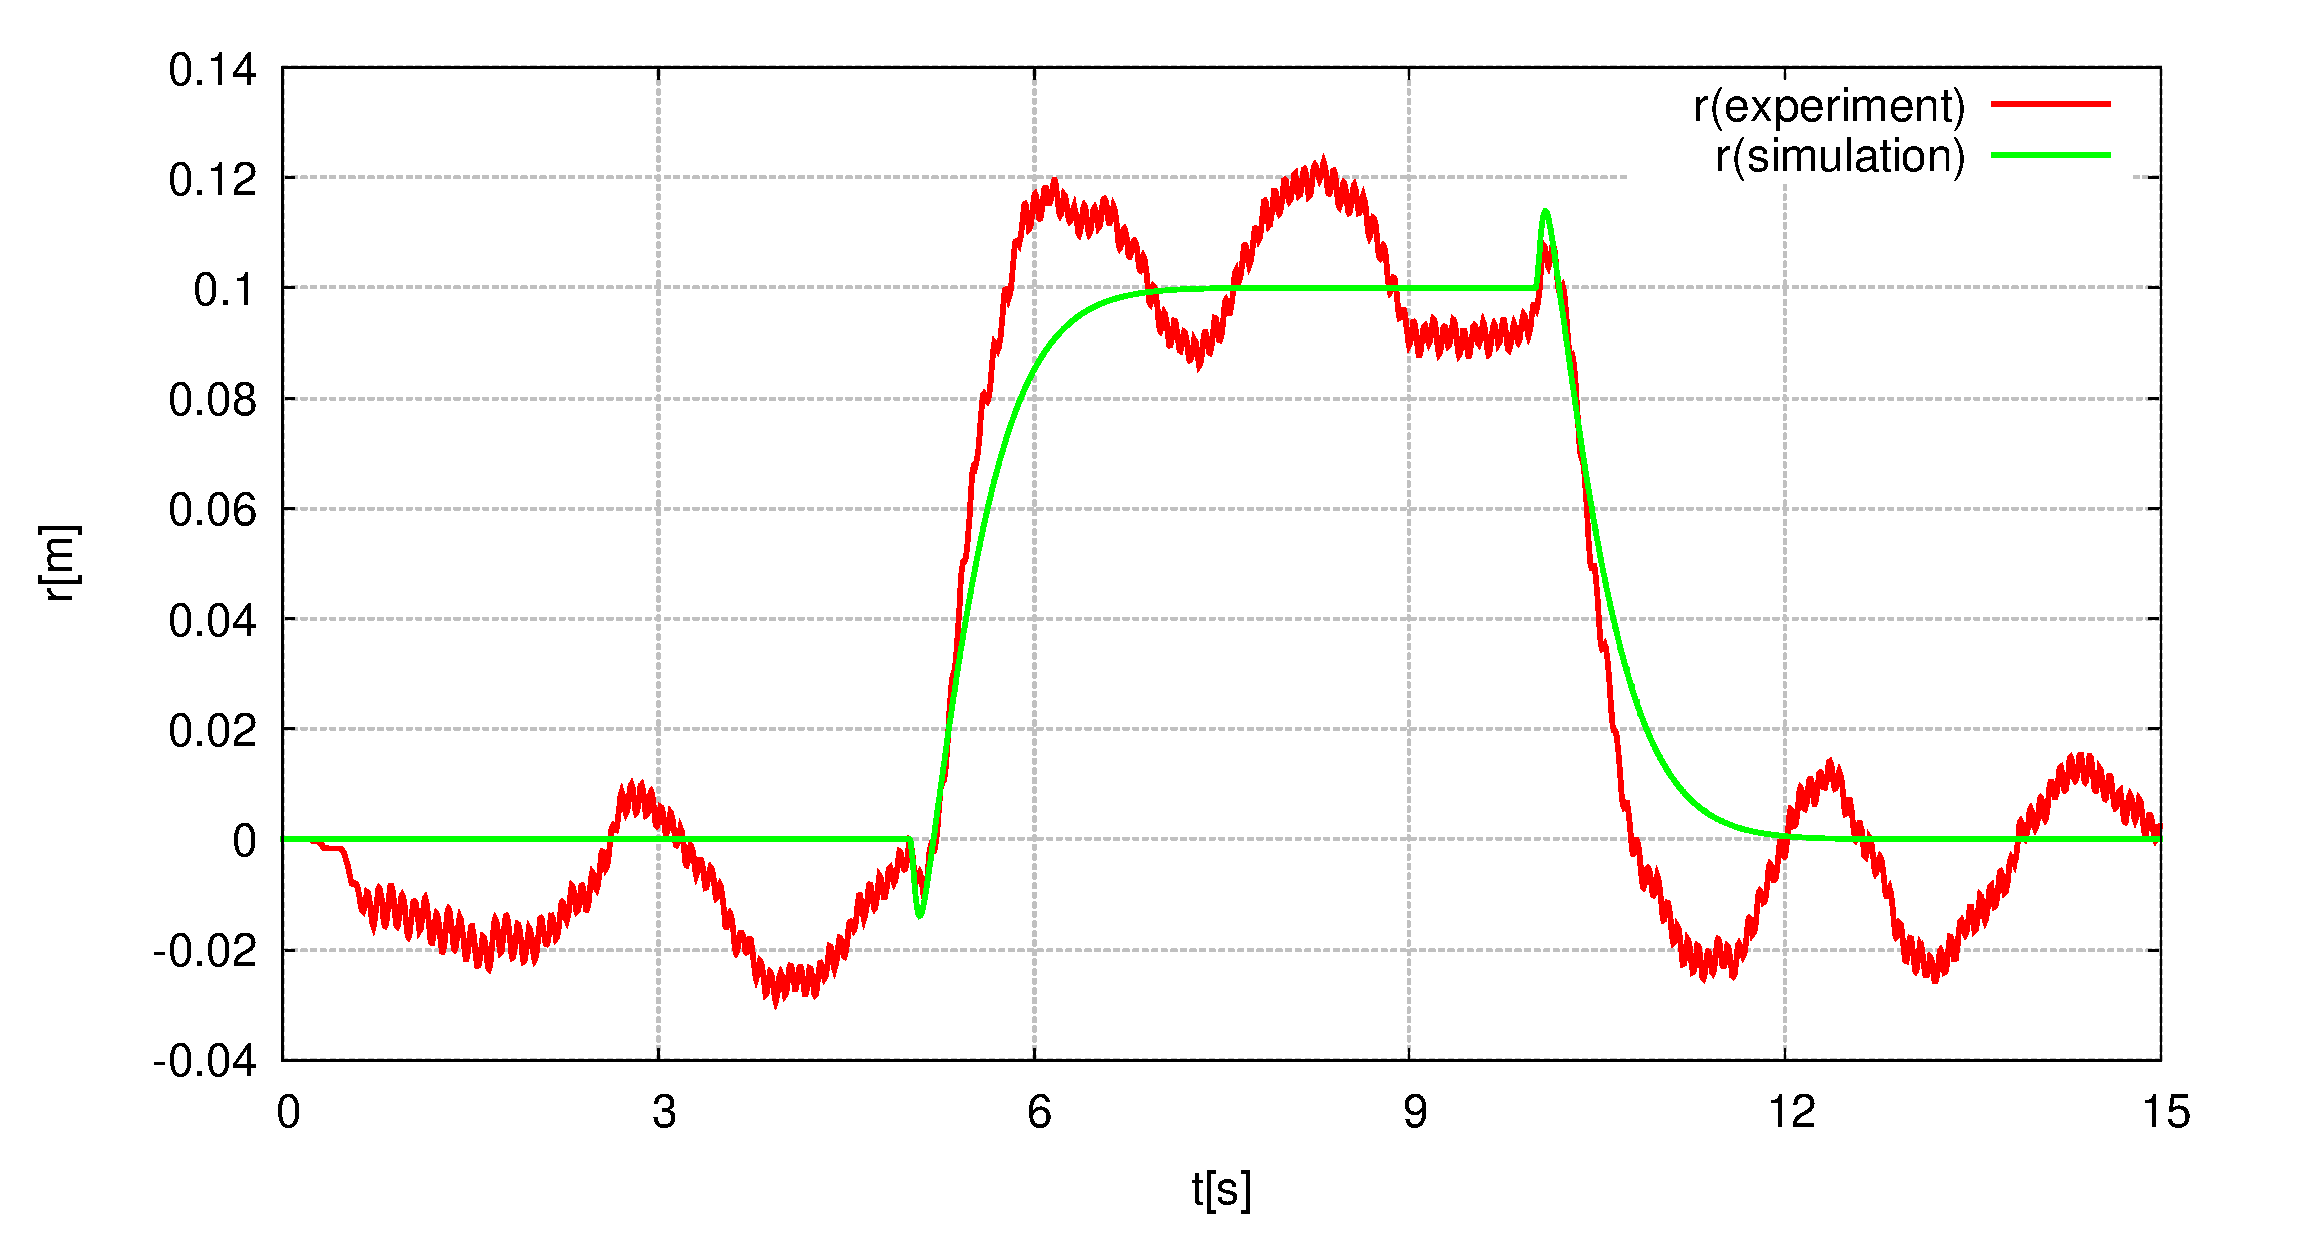
\includegraphics[width=0.49\linewidth]{gazo/experiment_Q55obs60dt05R2.eps}
		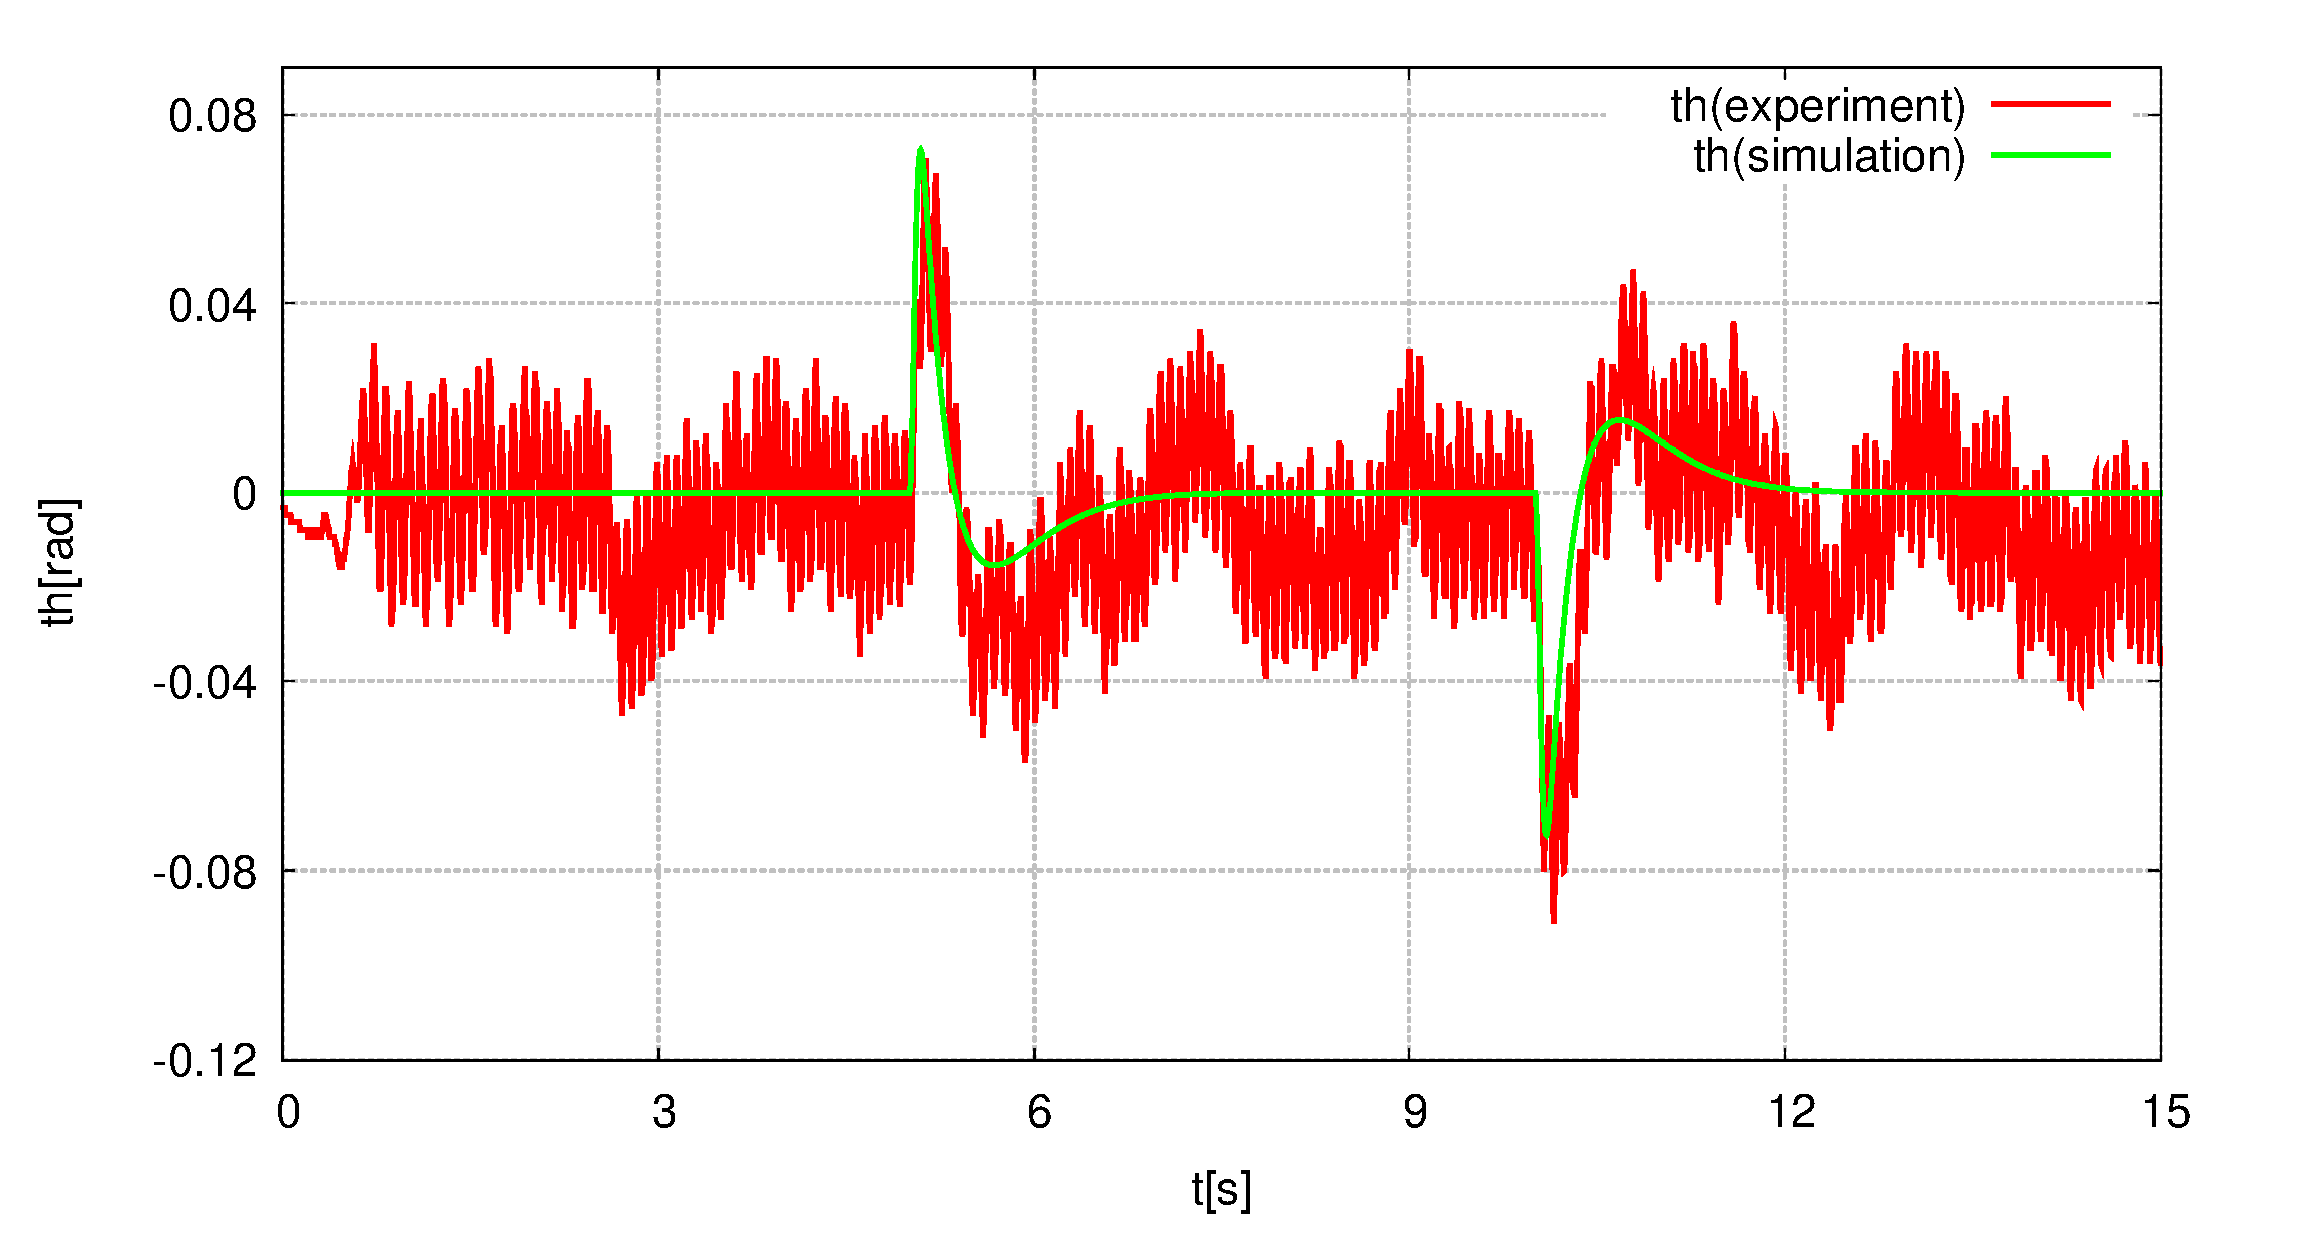
\includegraphics[width=0.49\linewidth]{gazo/experiment_Q55obs60dt05TH2.eps}
		\caption{比較結果その4(左図がr,右図が$\theta$)}
		\label{image:sono4}
	\end{figure}
	\begin{figure}[H]
		\centering
		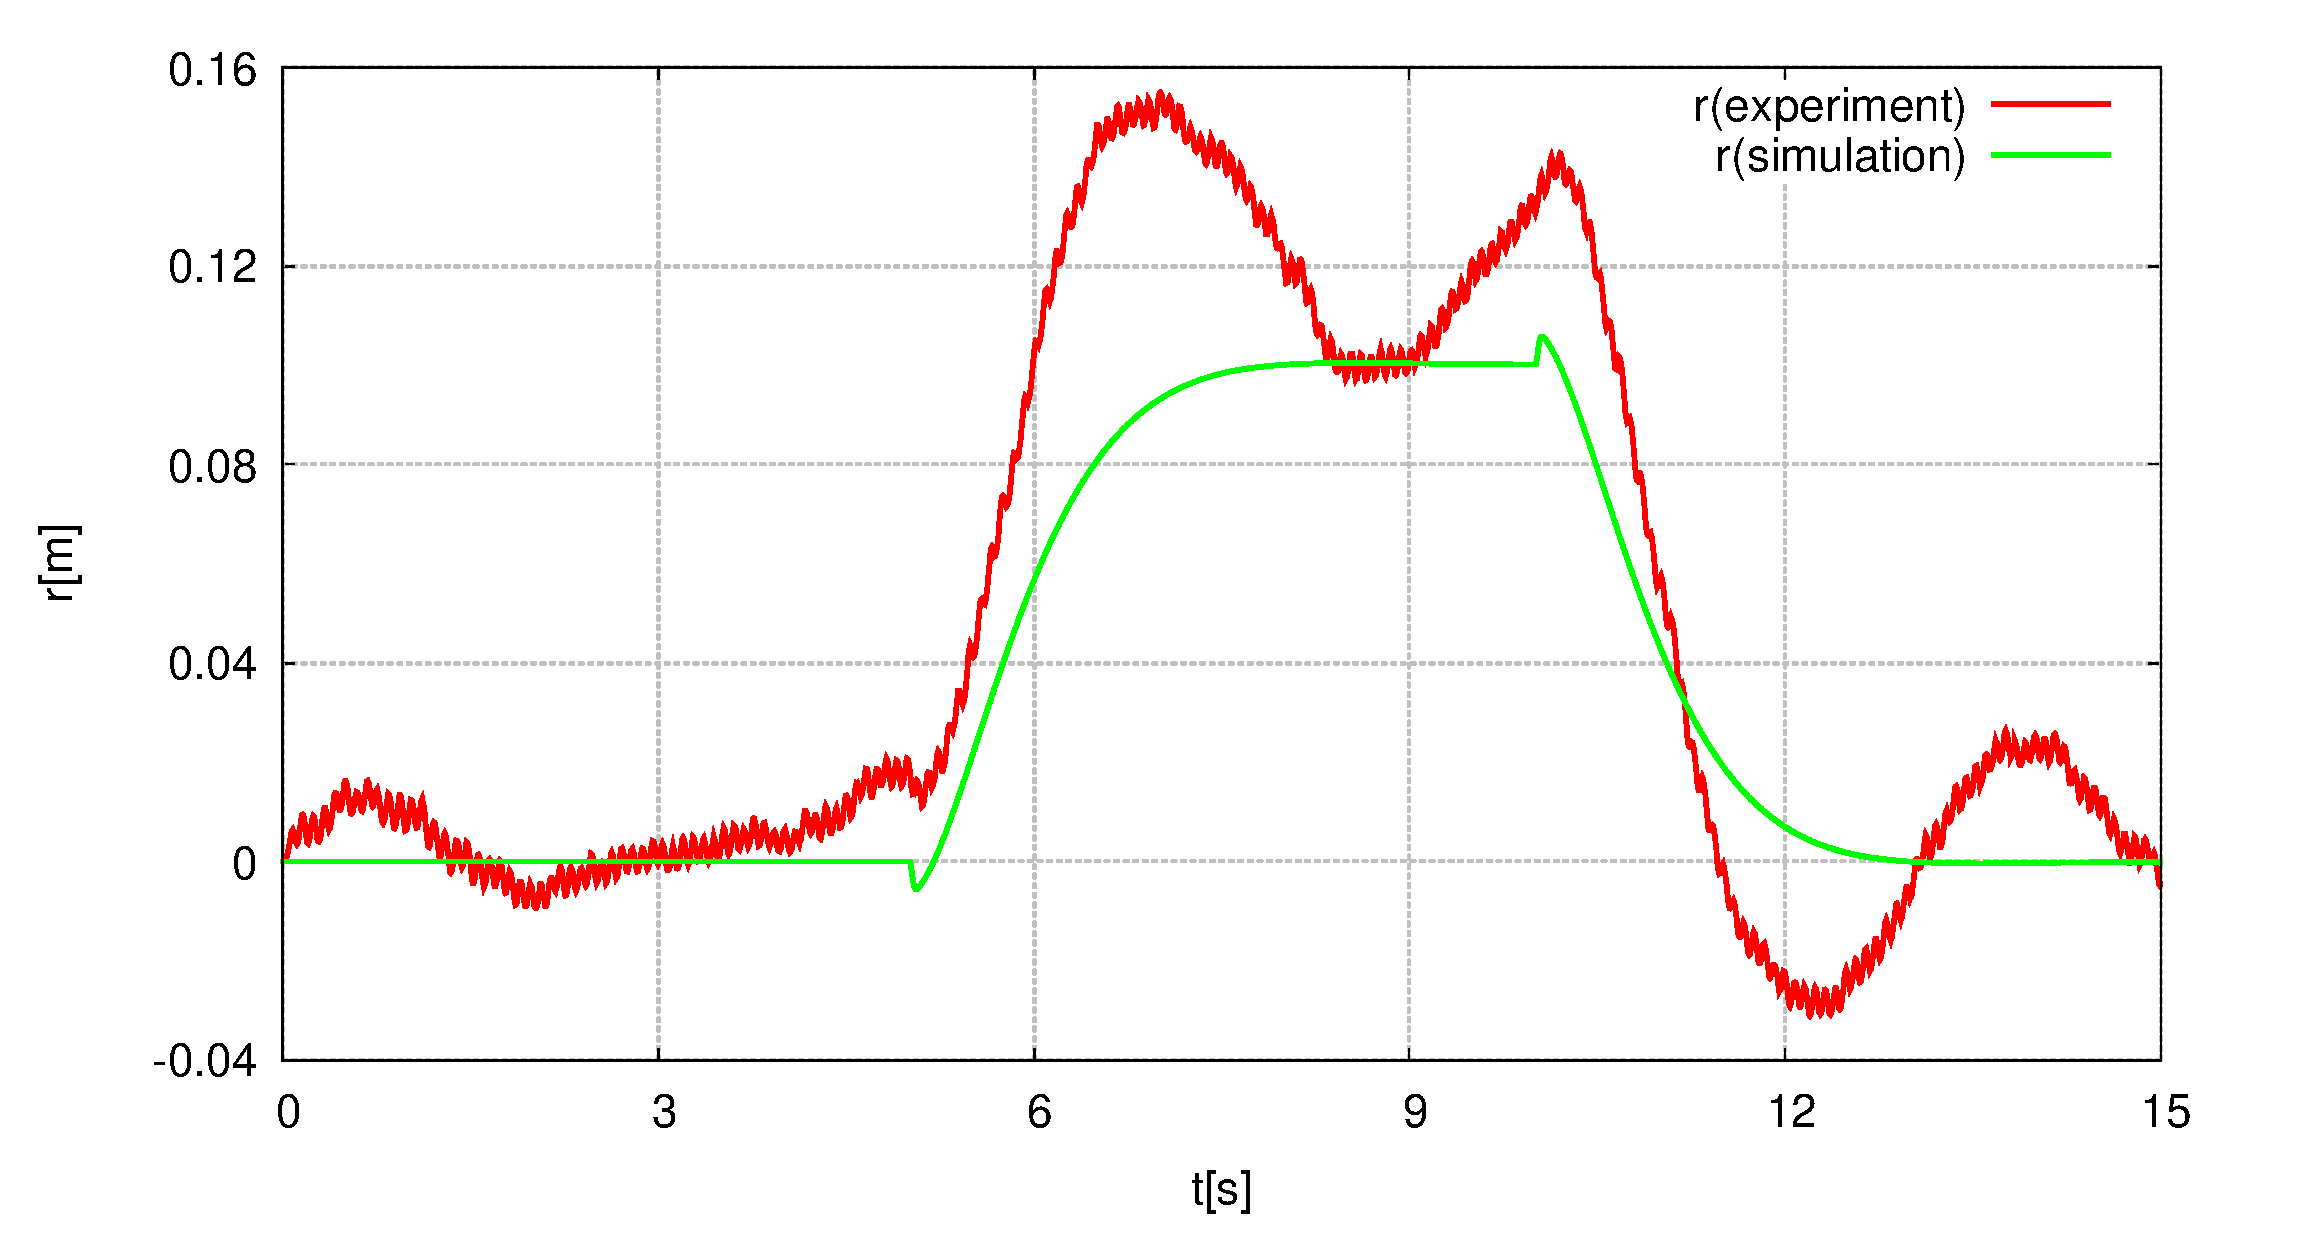
\includegraphics[width=0.49\linewidth]{gazo/experiment_Q56obs60dt05R2.eps}
		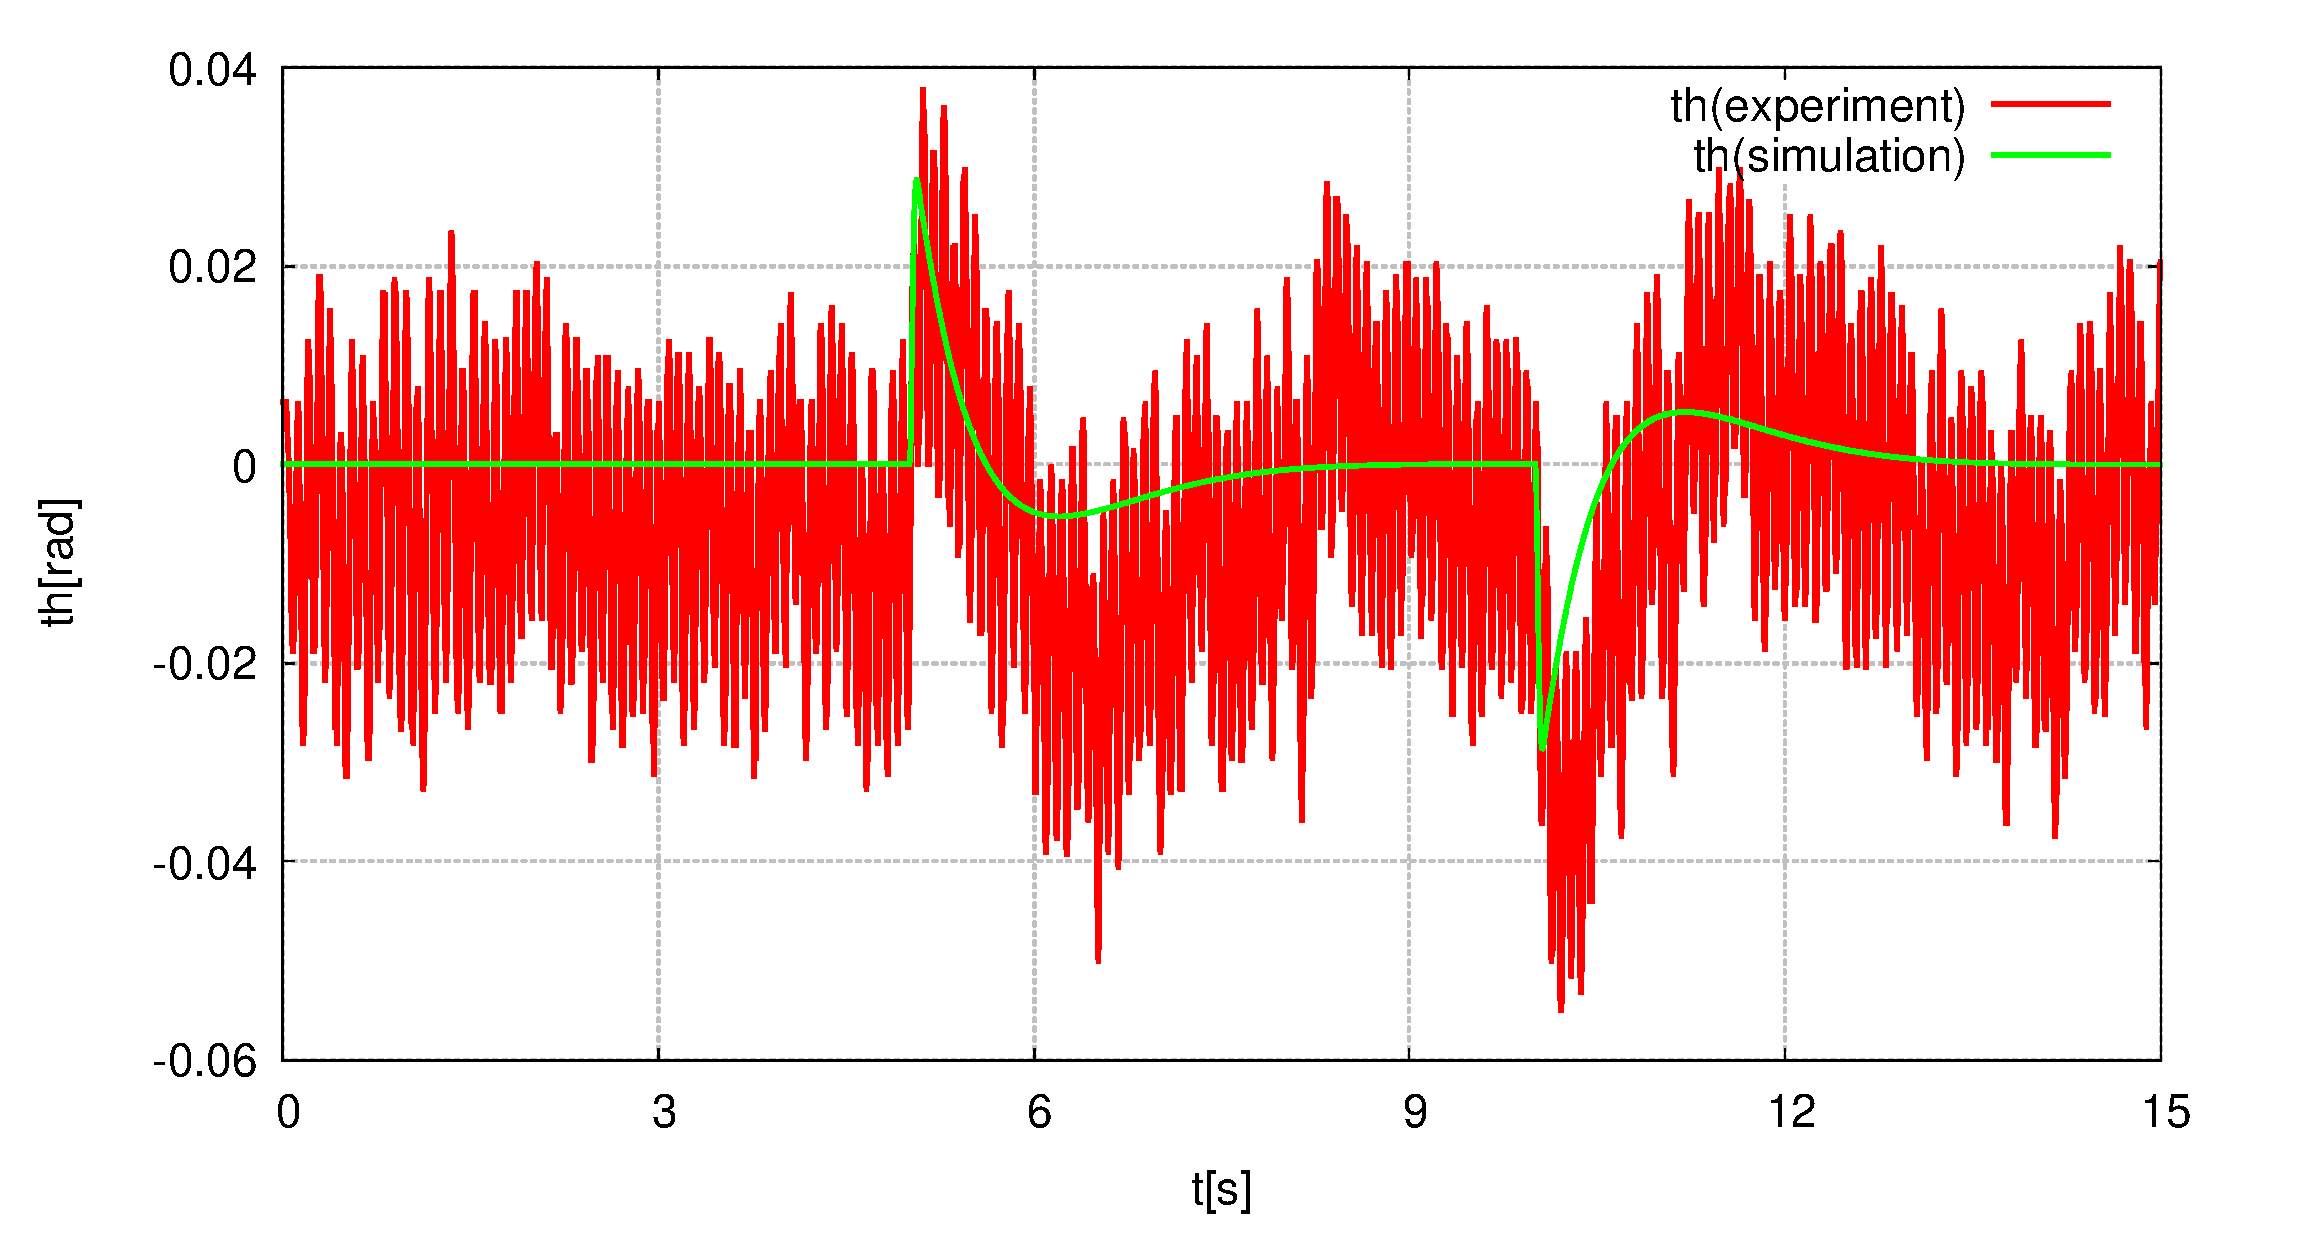
\includegraphics[width=0.49\linewidth]{gazo/experiment_Q56obs60dt05TH2.eps}
		\caption{比較結果その5(左図がr,右図が$\theta$)}
		\label{image:sono5}
	\end{figure}
	\begin{figure}[H]
		\centering
		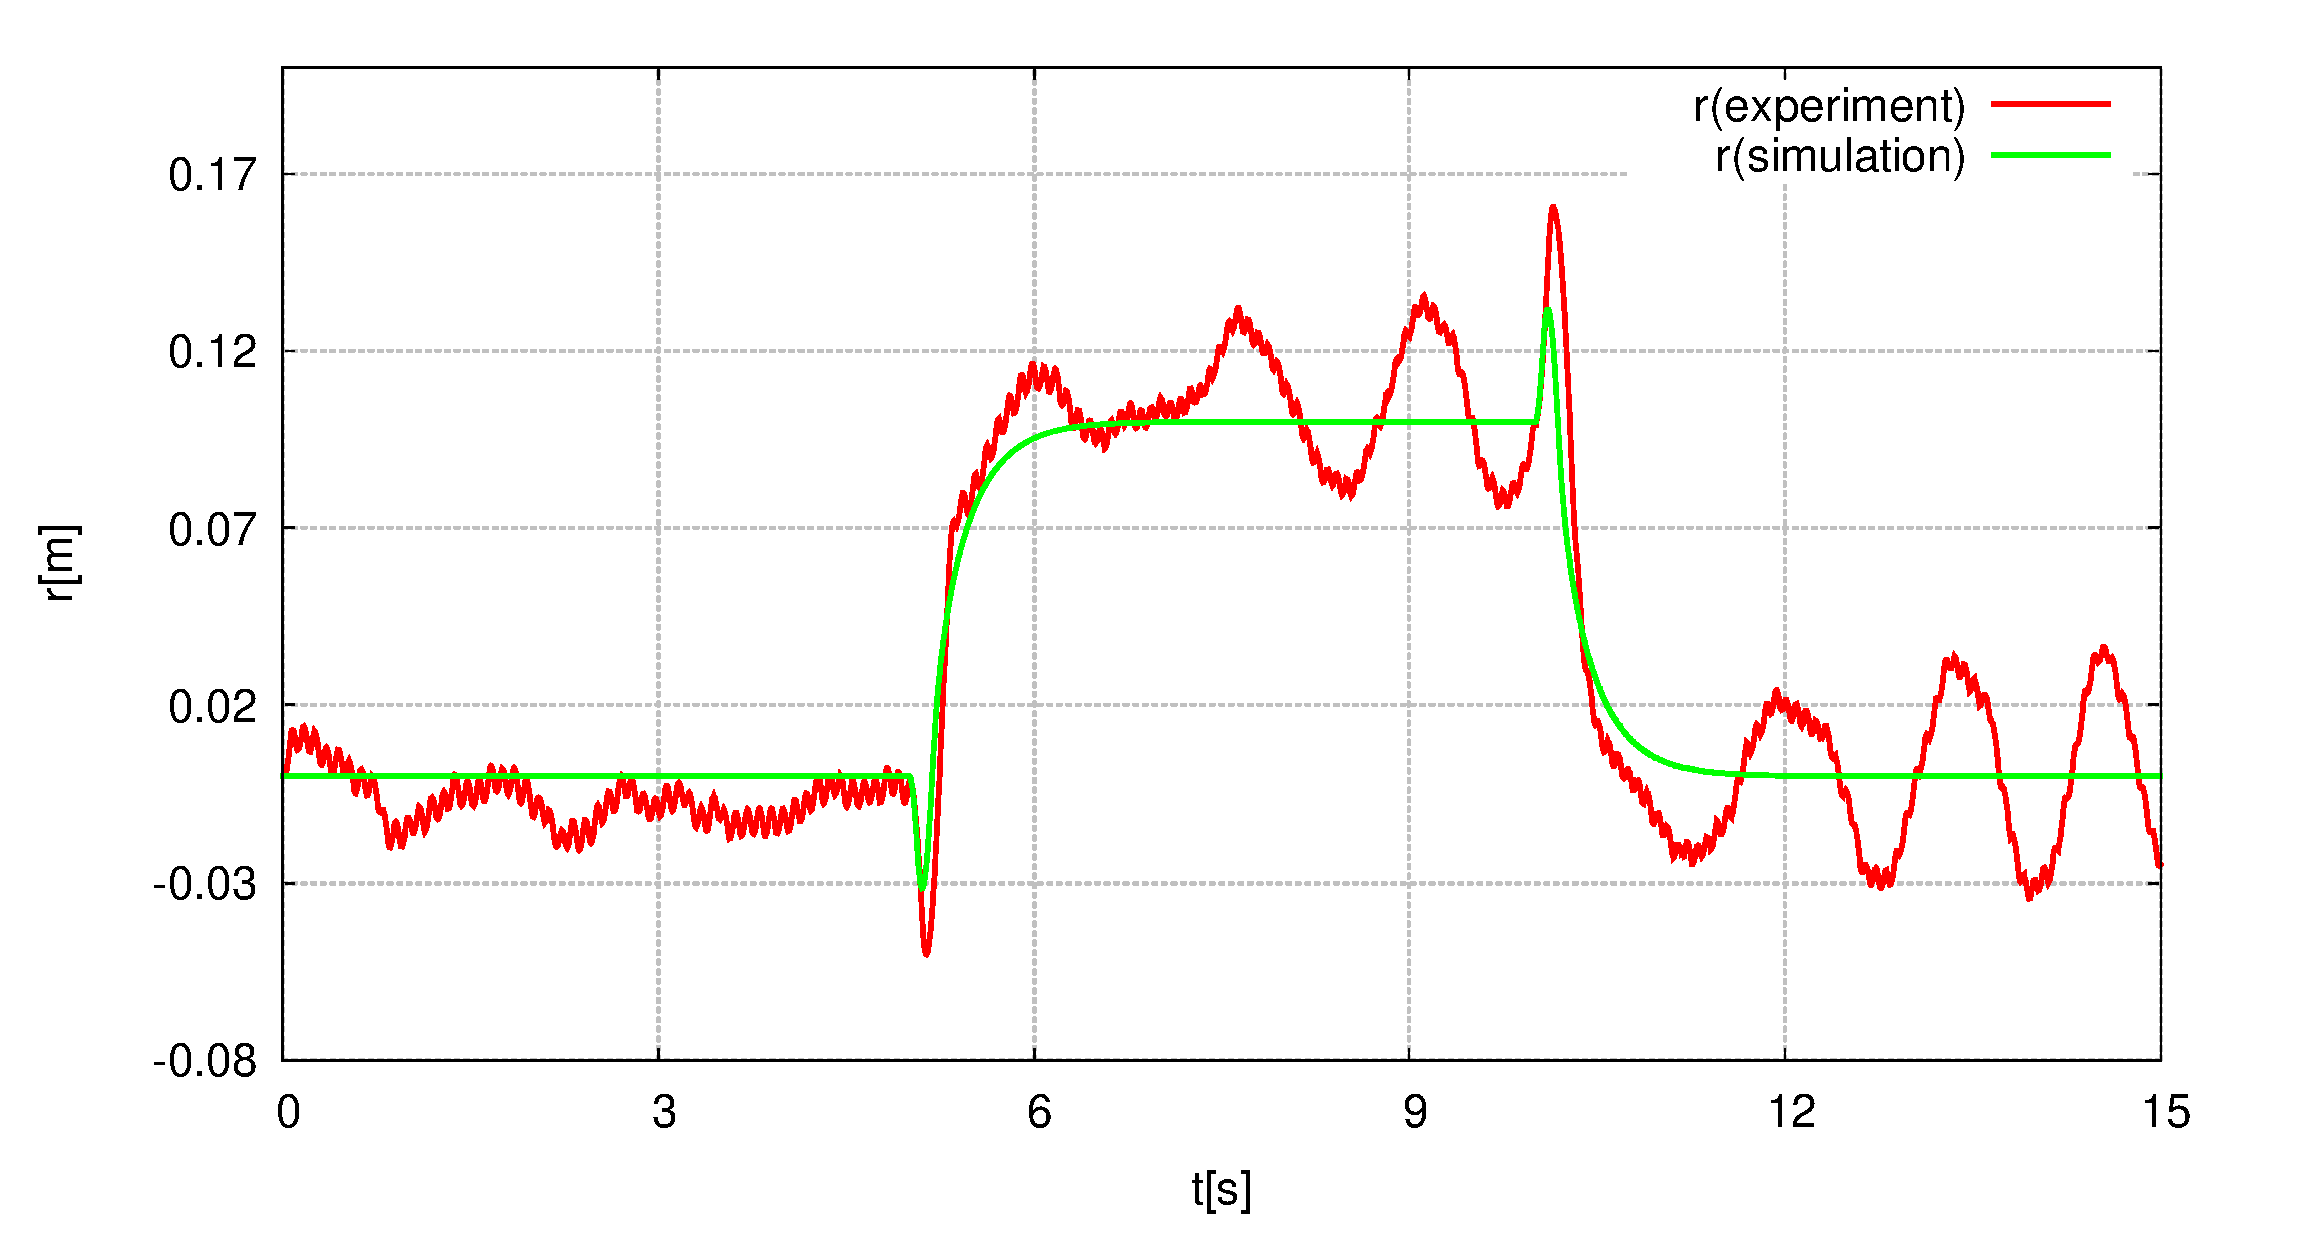
\includegraphics[width=0.49\linewidth]{gazo/experiment_Q65obs60dt05R2.eps}
		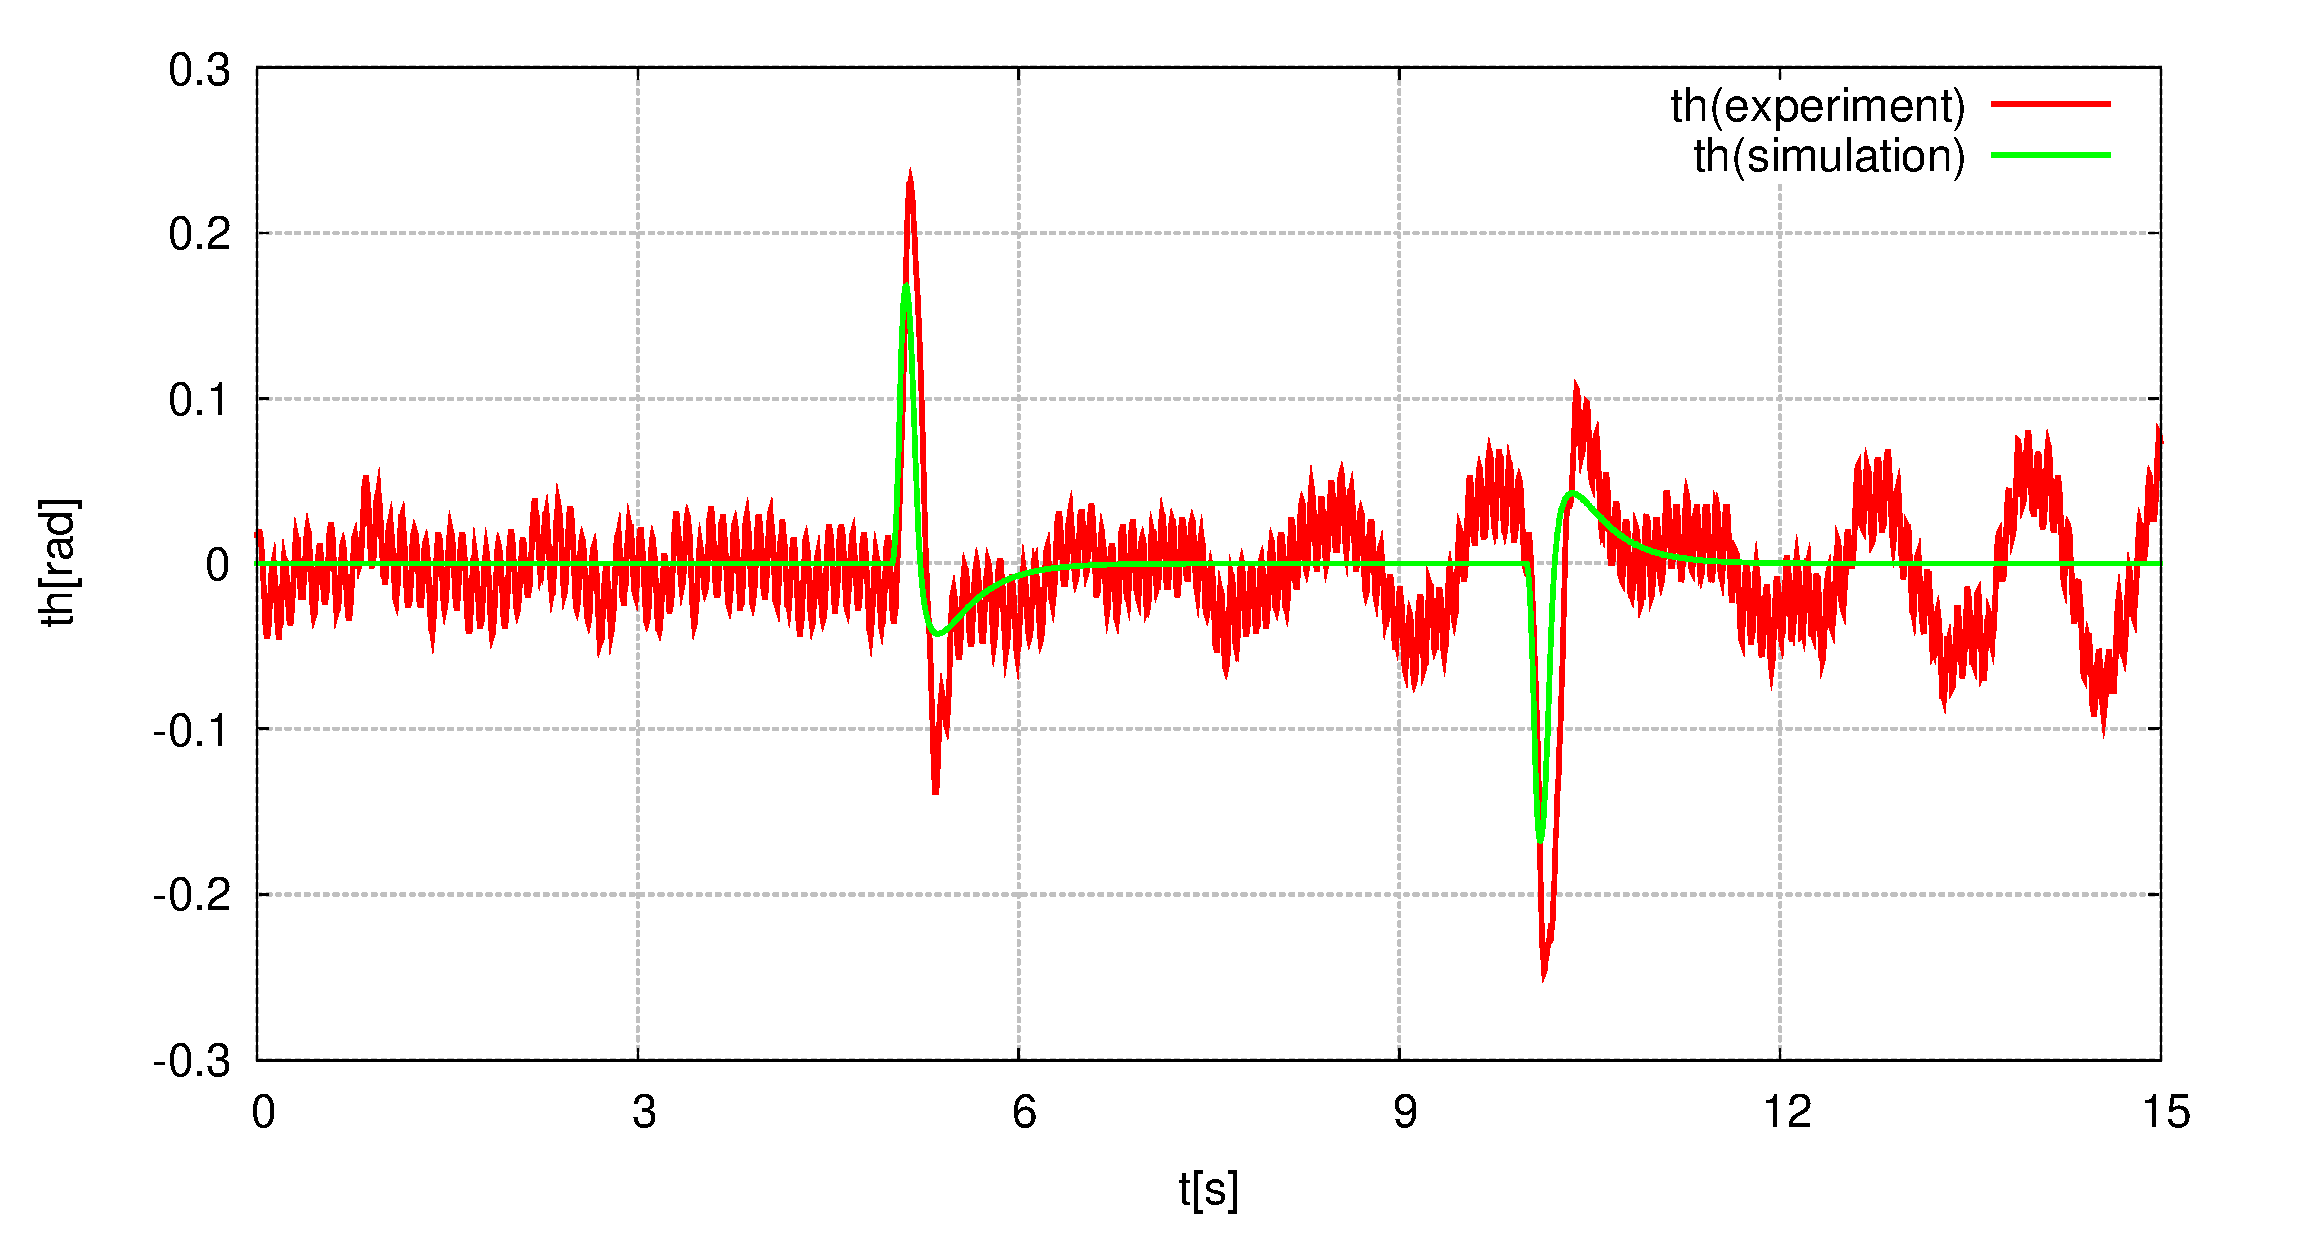
\includegraphics[width=0.49\linewidth]{gazo/experiment_Q65obs60dt05TH2.eps}
		\caption{比較結果その6(左図がr,右図が$\theta$)}
		\label{image:sono6}
	\end{figure}
	\begin{figure}[H]
		\centering
		\includegraphics[width=0.49\linewidth]{gazo/experiment_Q55obs30dt10R2.eps}
		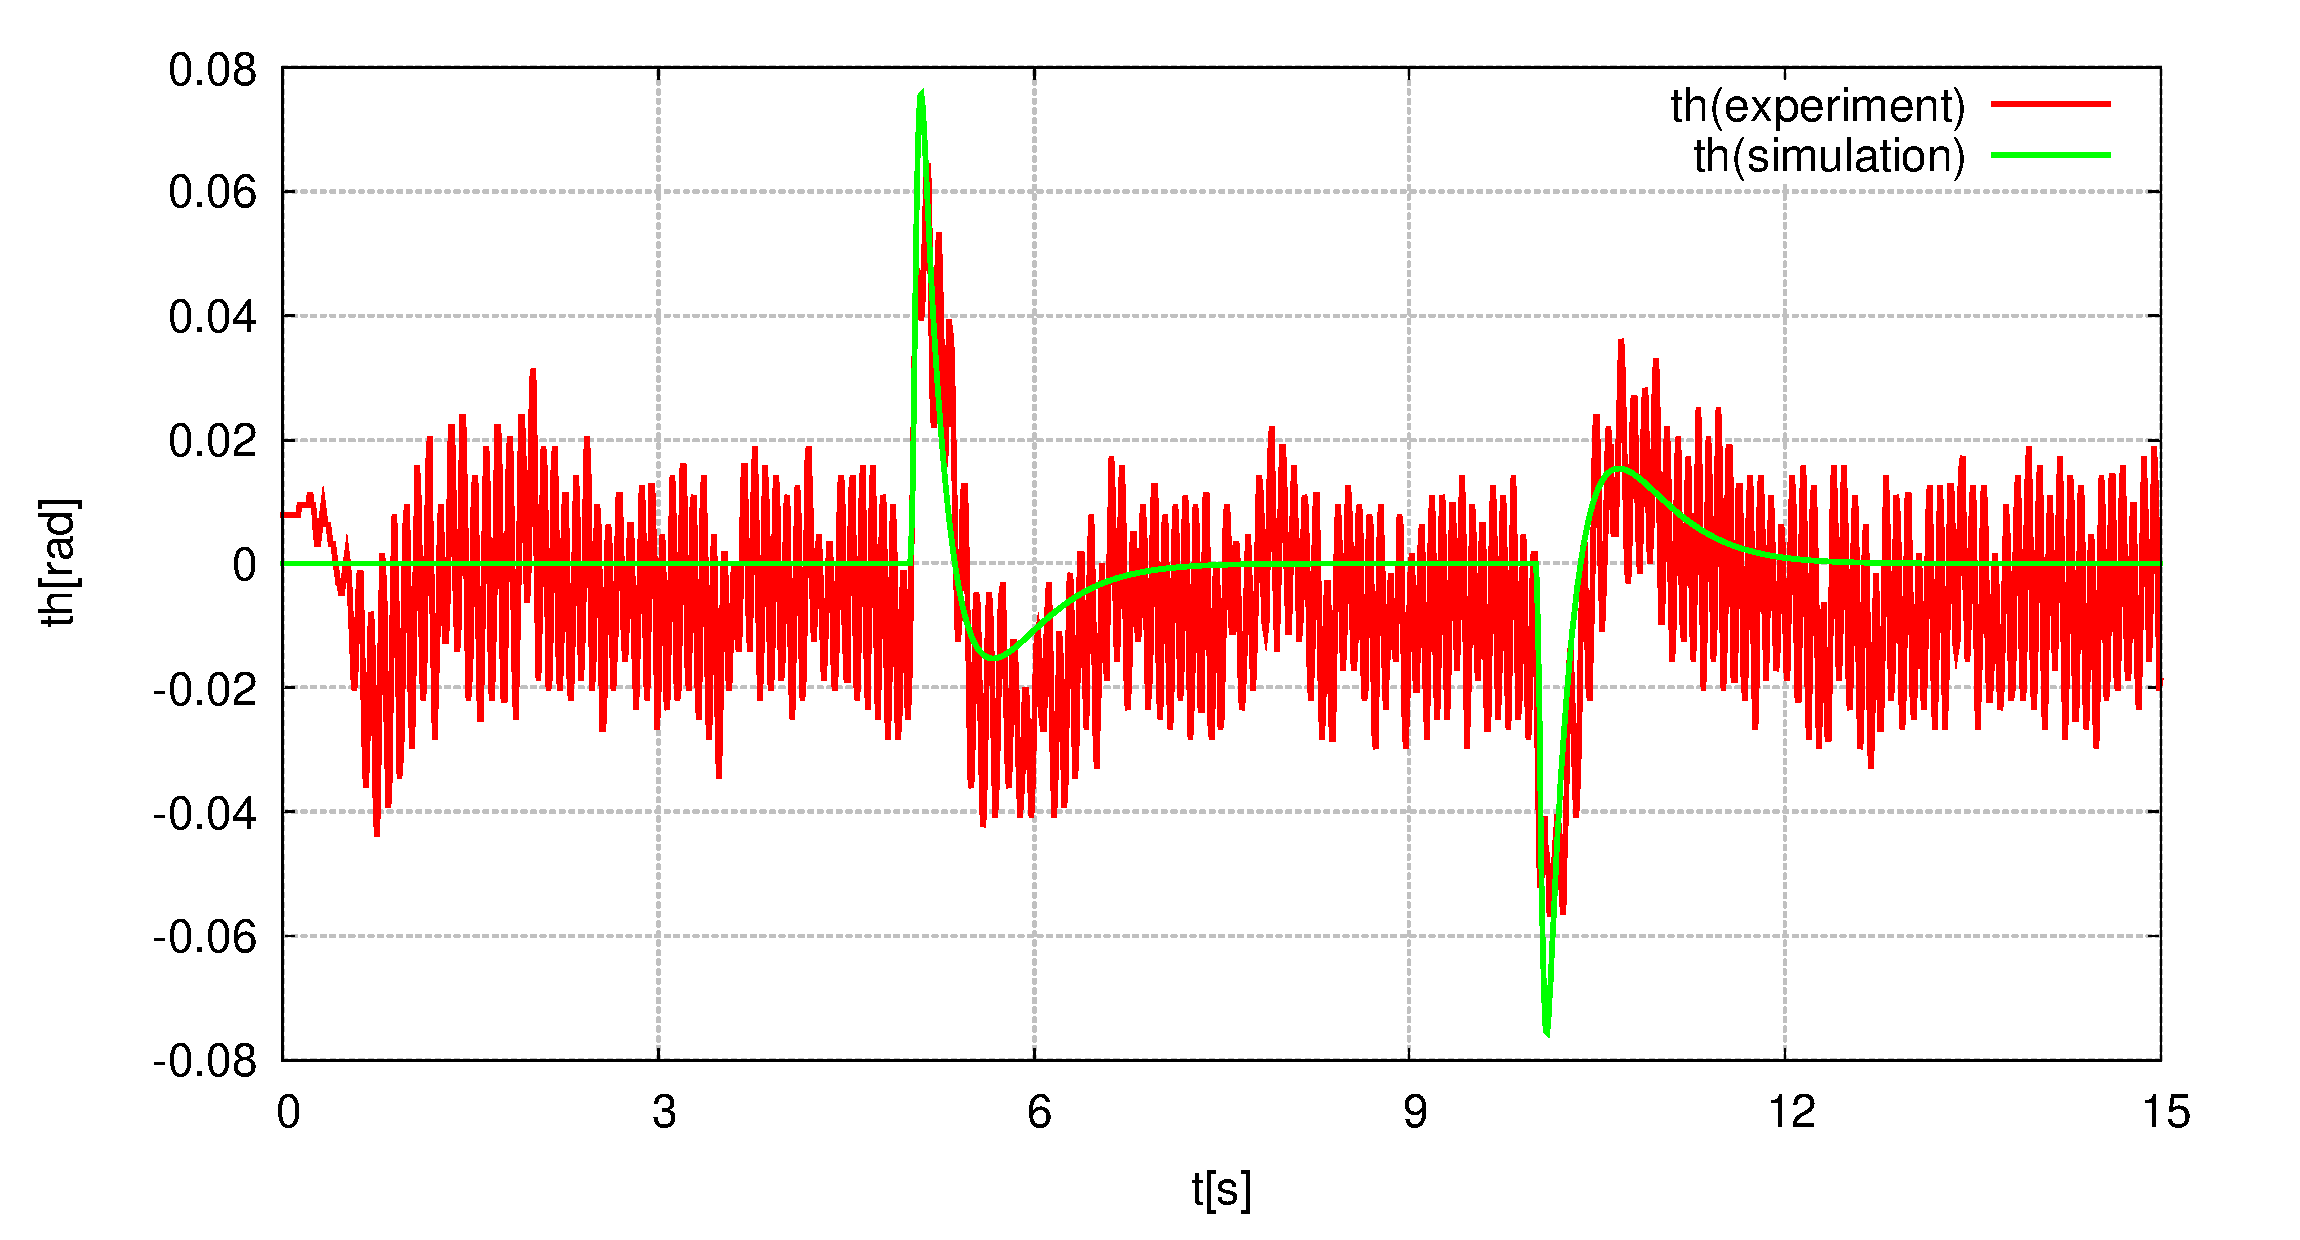
\includegraphics[width=0.49\linewidth]{gazo/experiment_Q55obs30dt10TH2.eps}
		\caption{比較結果その7(左図がr,右図が$\theta$)}
		\label{image:sono7}
	\end{figure}
	\begin{figure}[H]
		\centering
		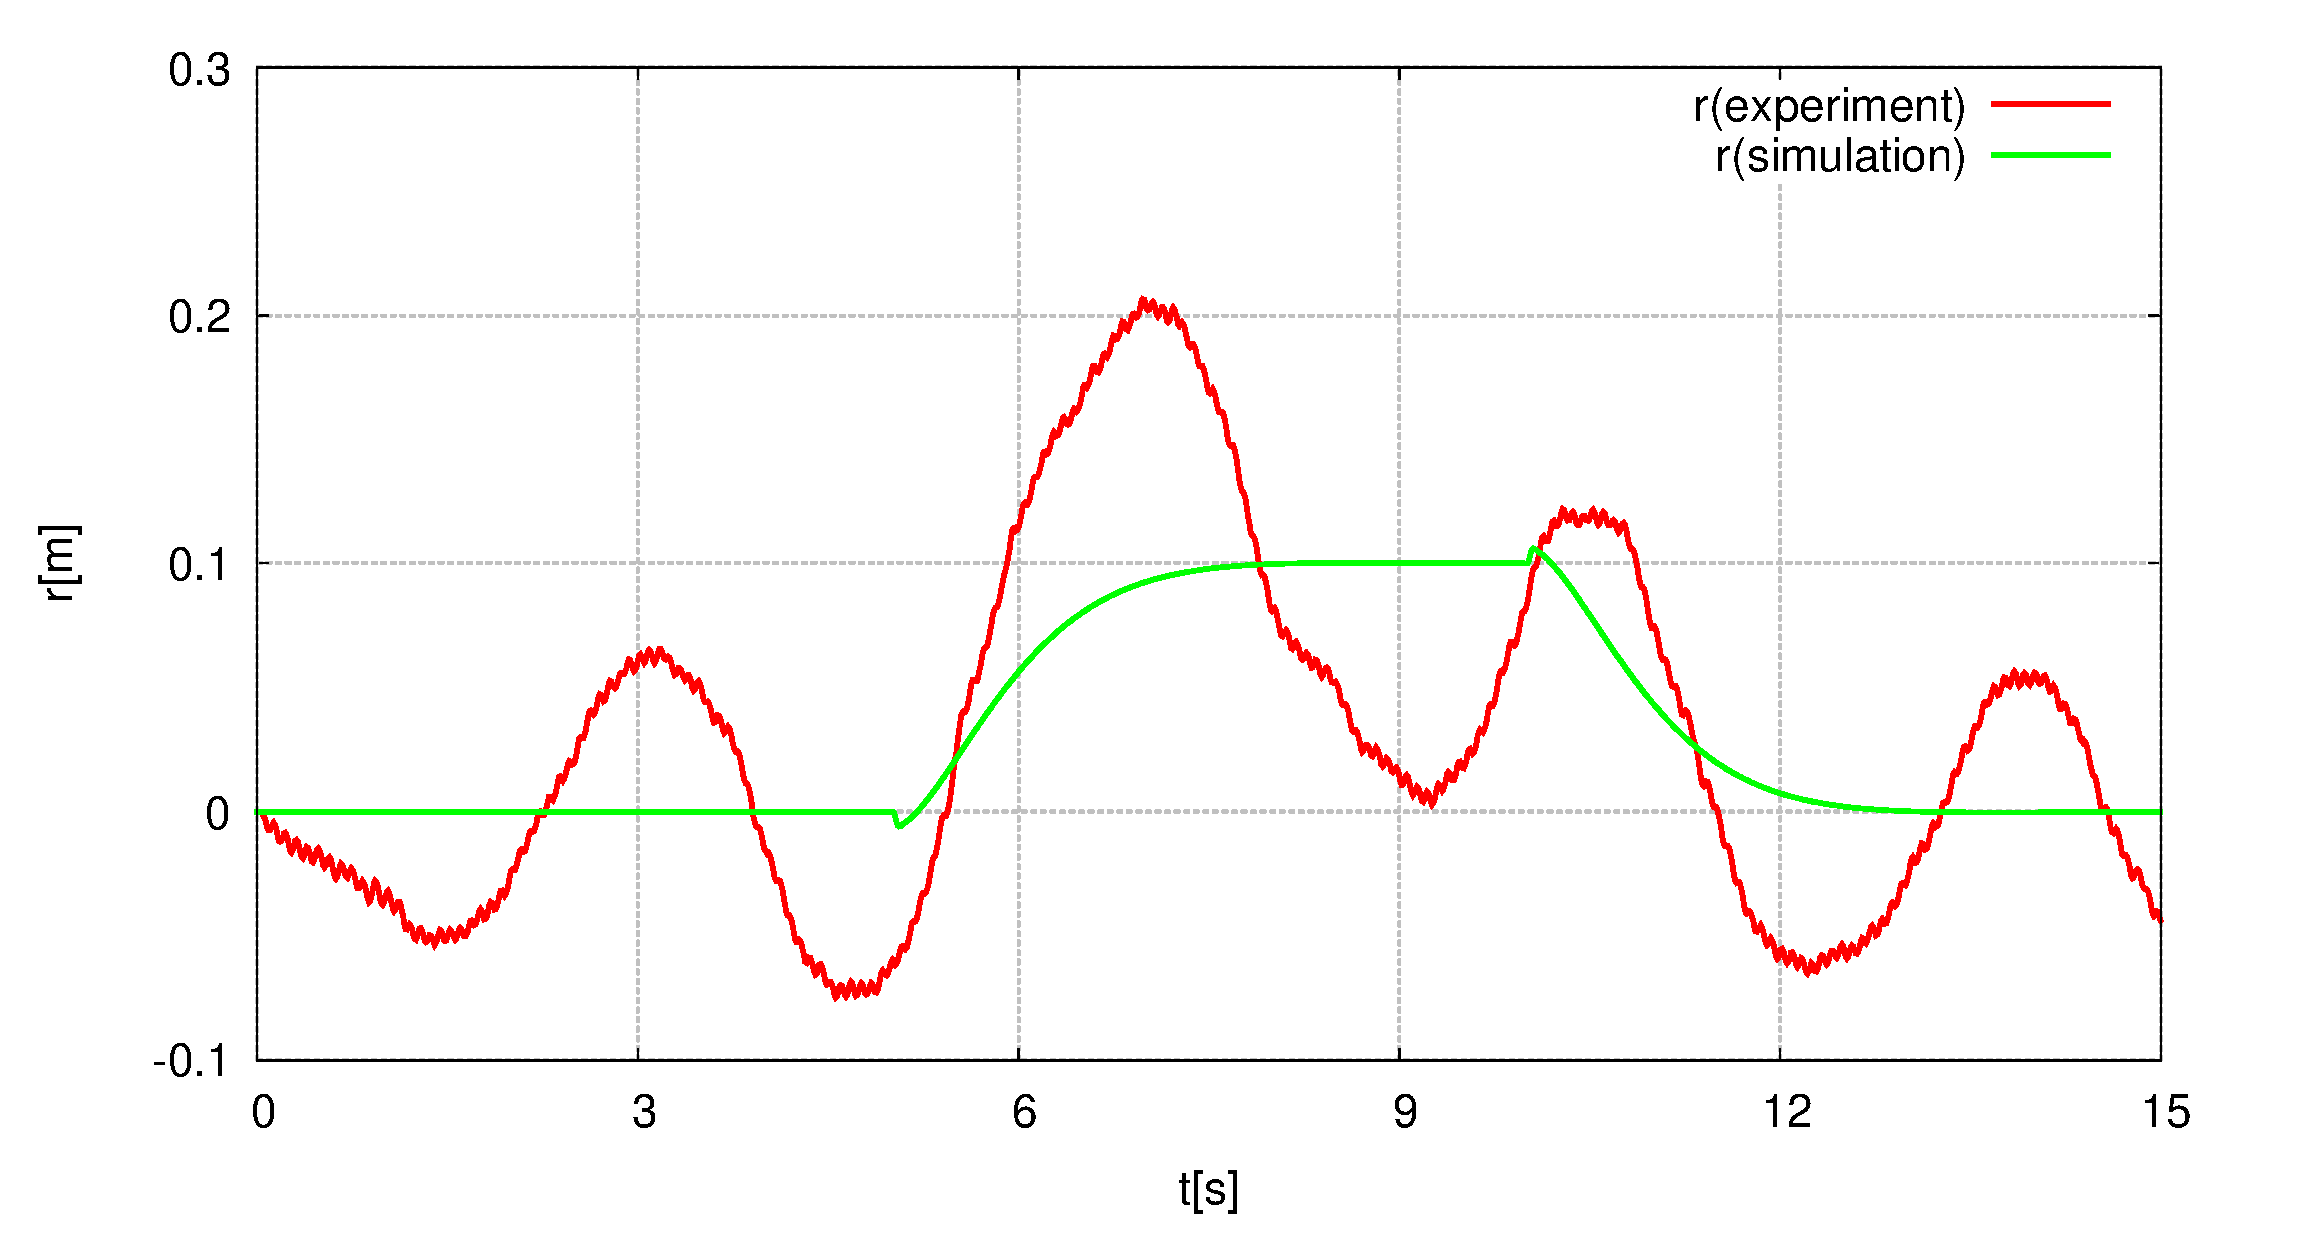
\includegraphics[width=0.49\linewidth]{gazo/experiment_Q56obs30dt10R2.eps}
		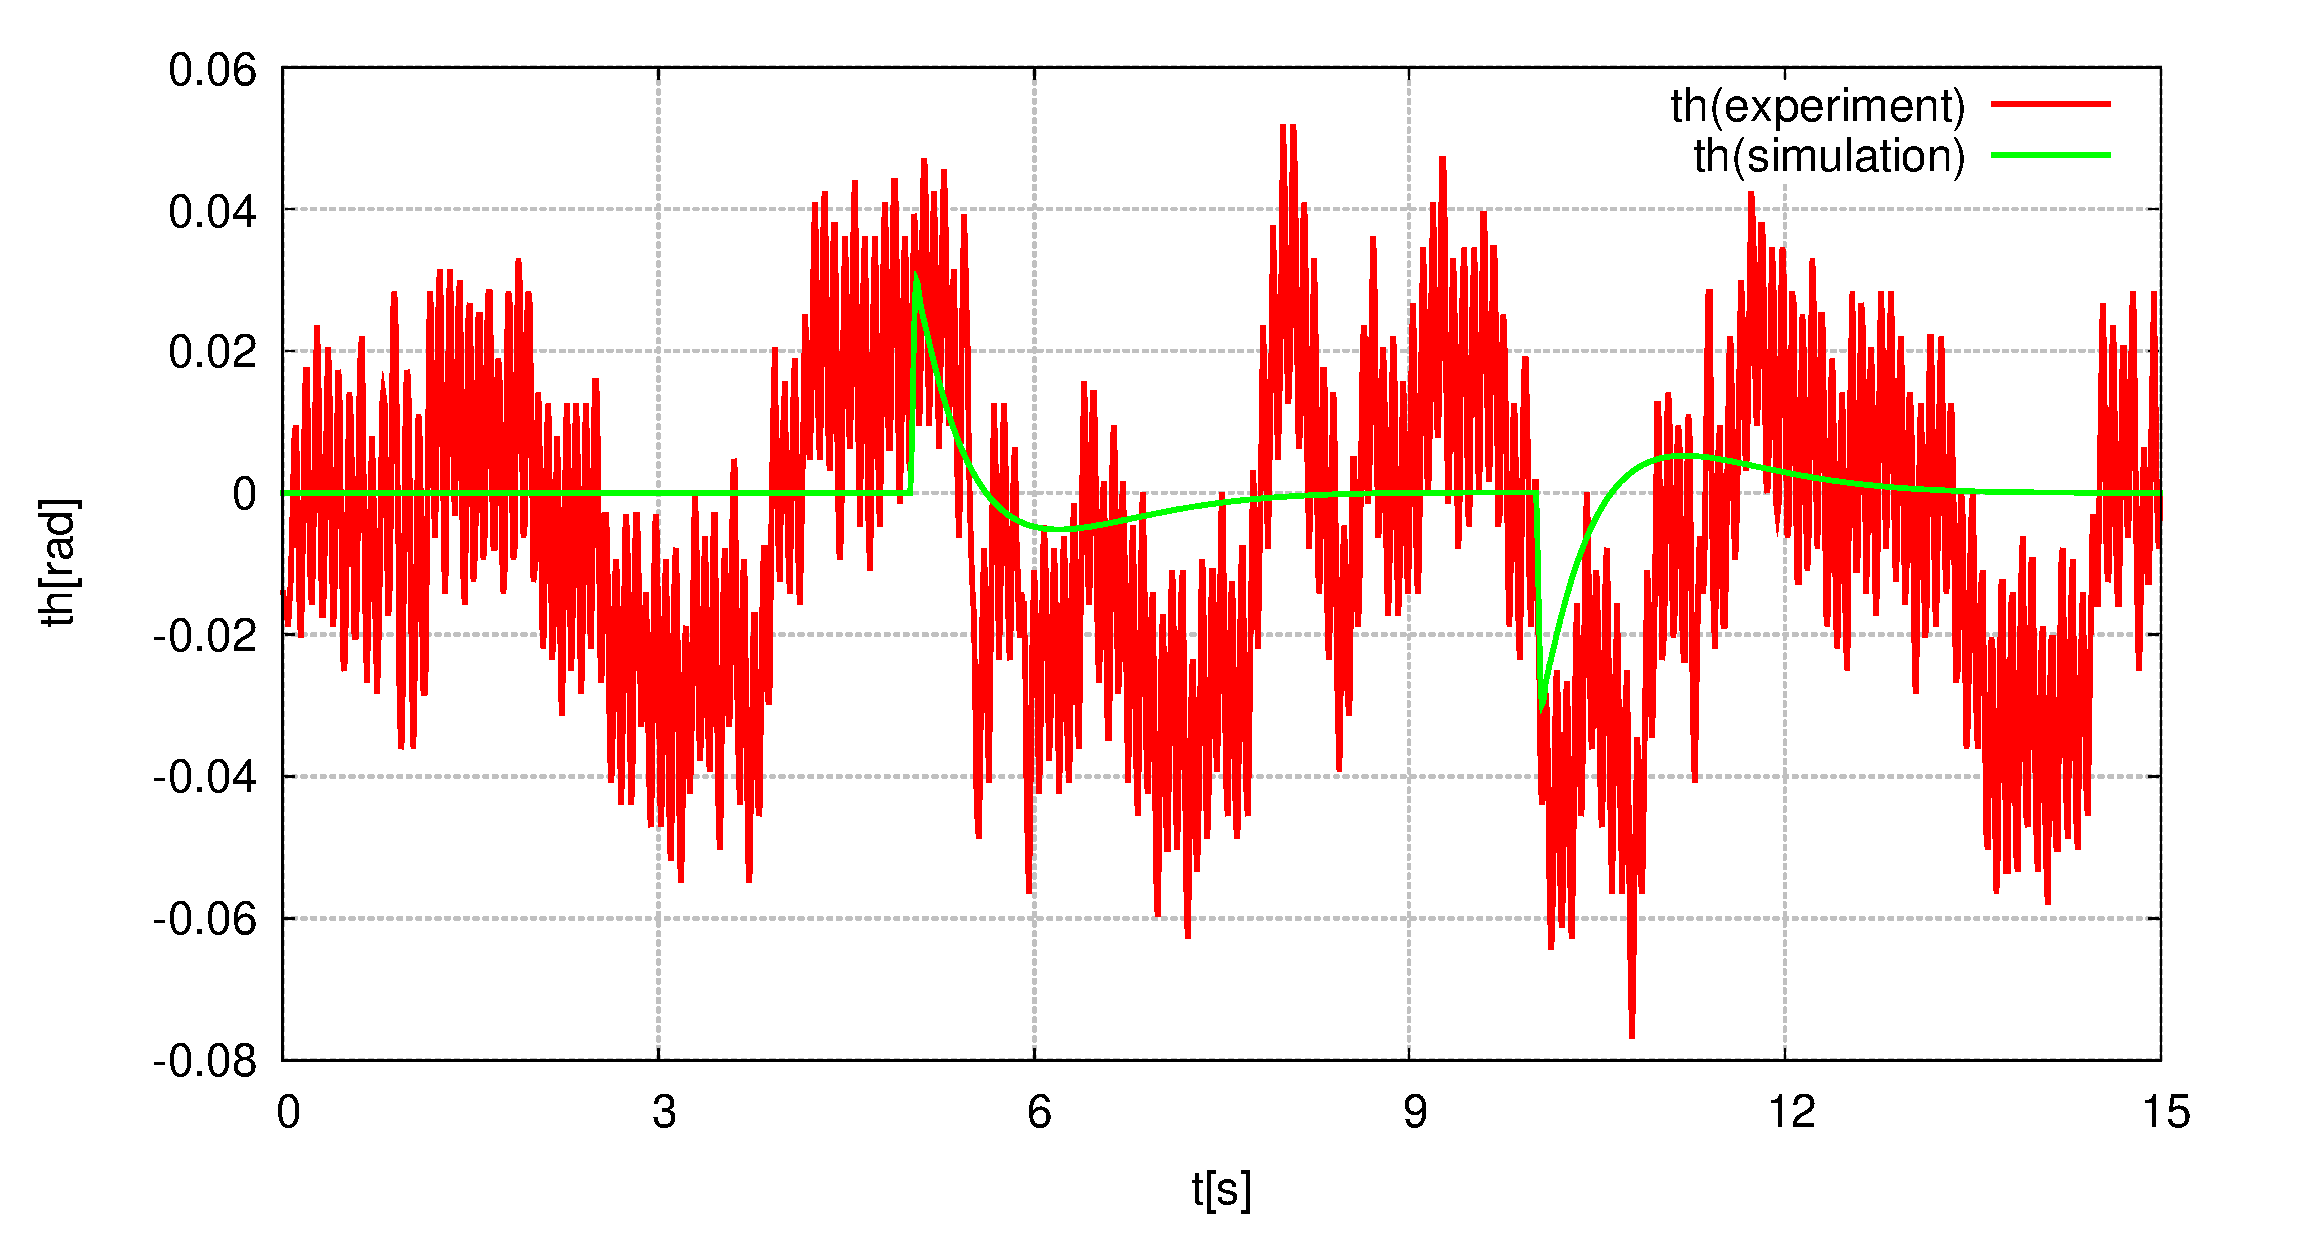
\includegraphics[width=0.49\linewidth]{gazo/experiment_Q56obs30dt10TH2.eps}
		\caption{比較結果その8(左図がr,右図が$\theta$)}
		\label{image:sono8}
	\end{figure}
	\begin{figure}[H]
		\centering
		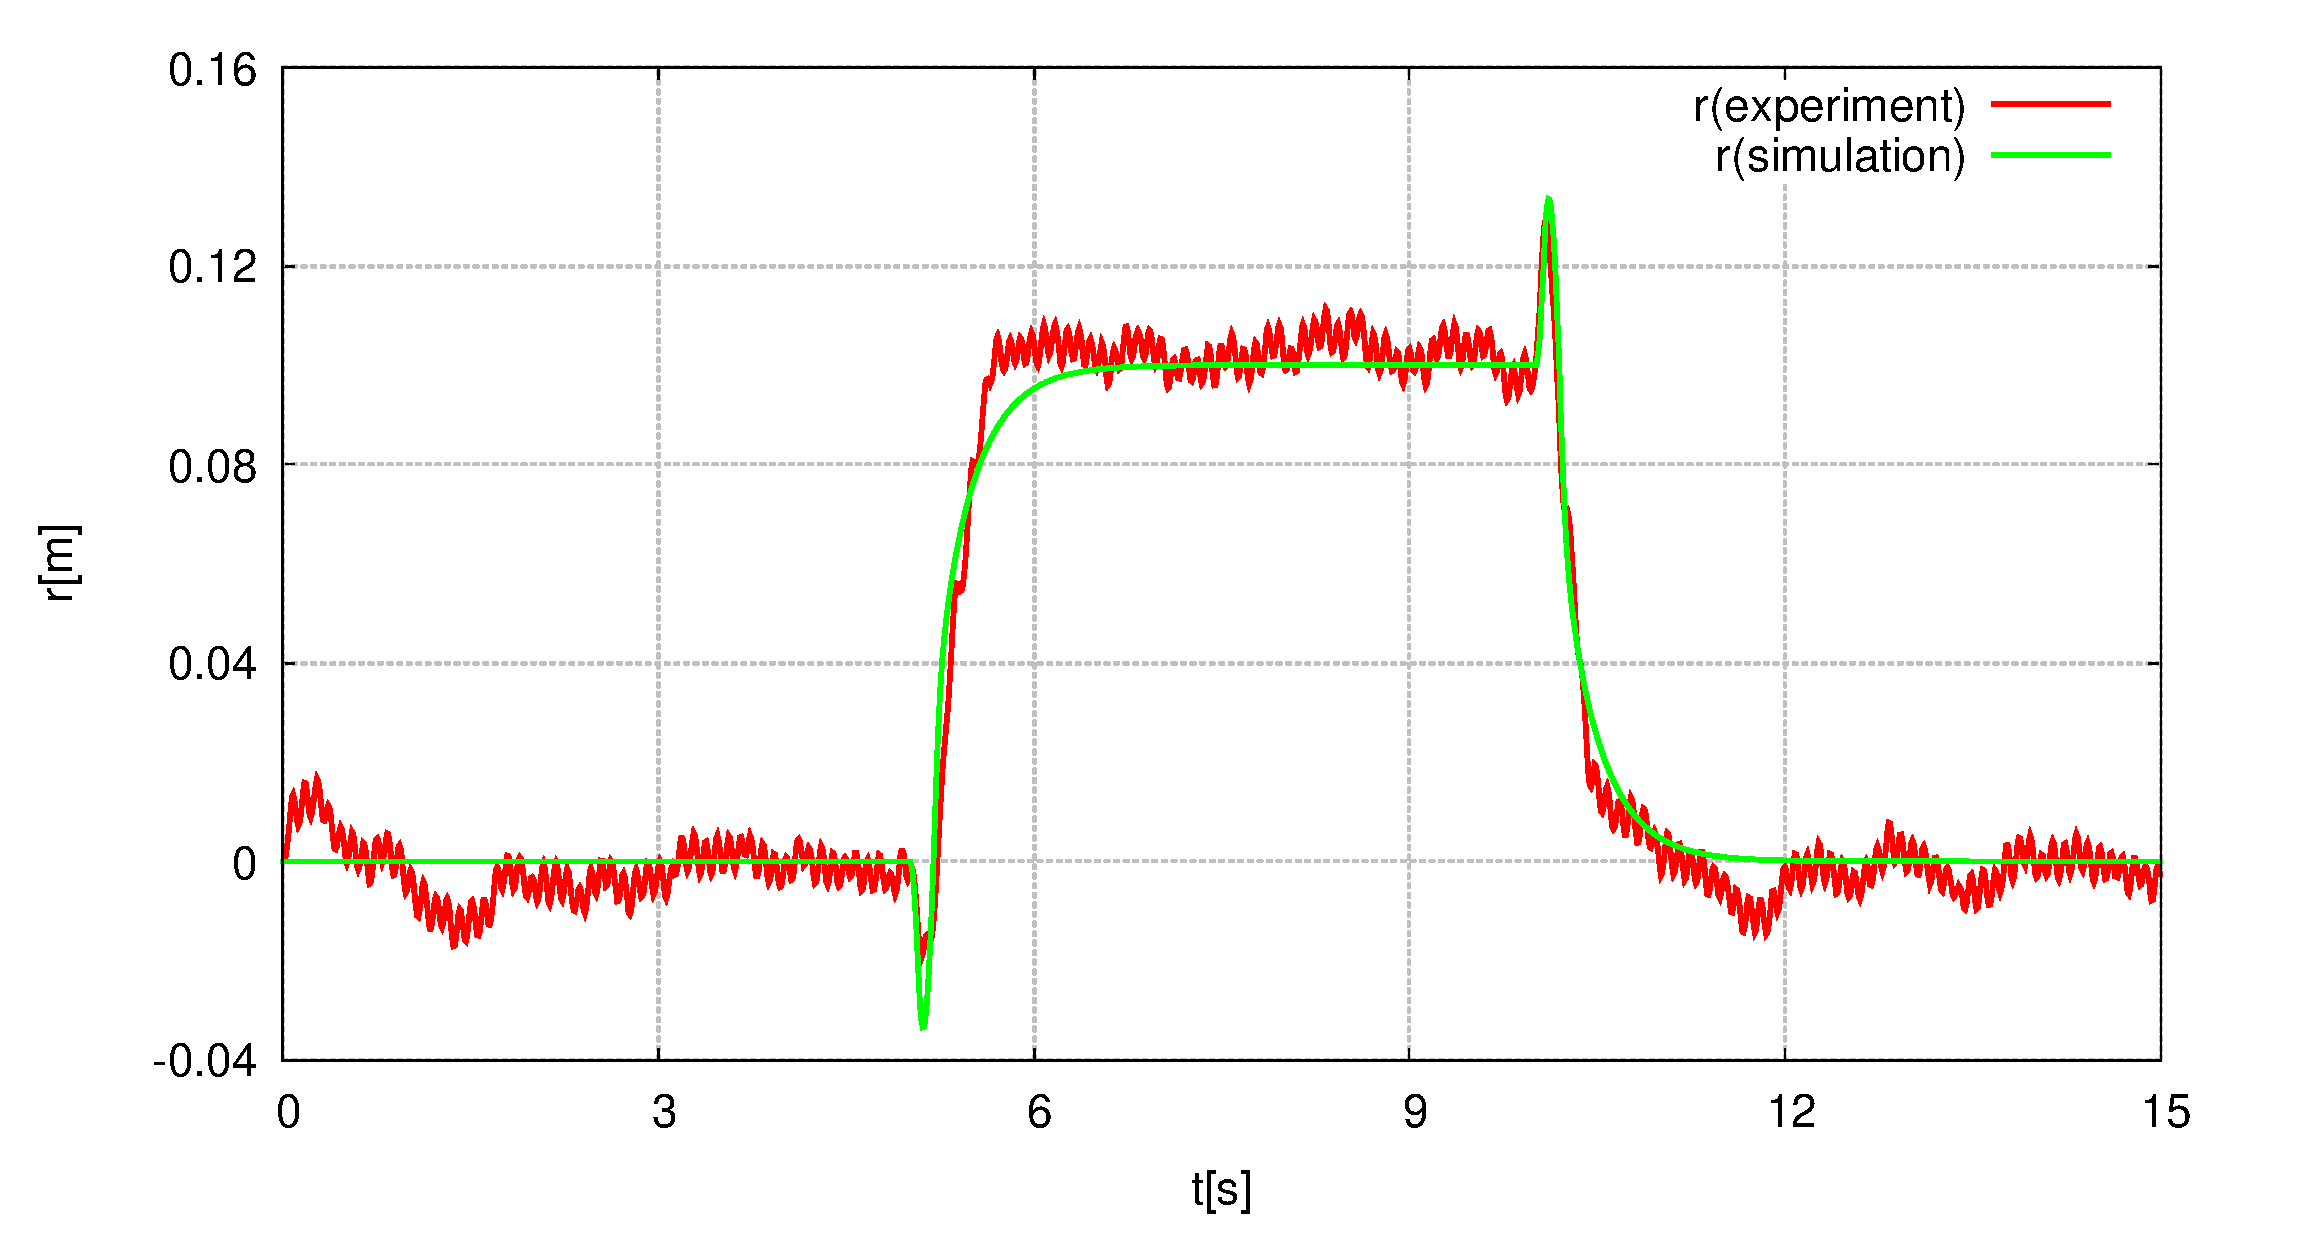
\includegraphics[width=0.49\linewidth]{gazo/experiment_Q65obs30dt10R2.eps}
		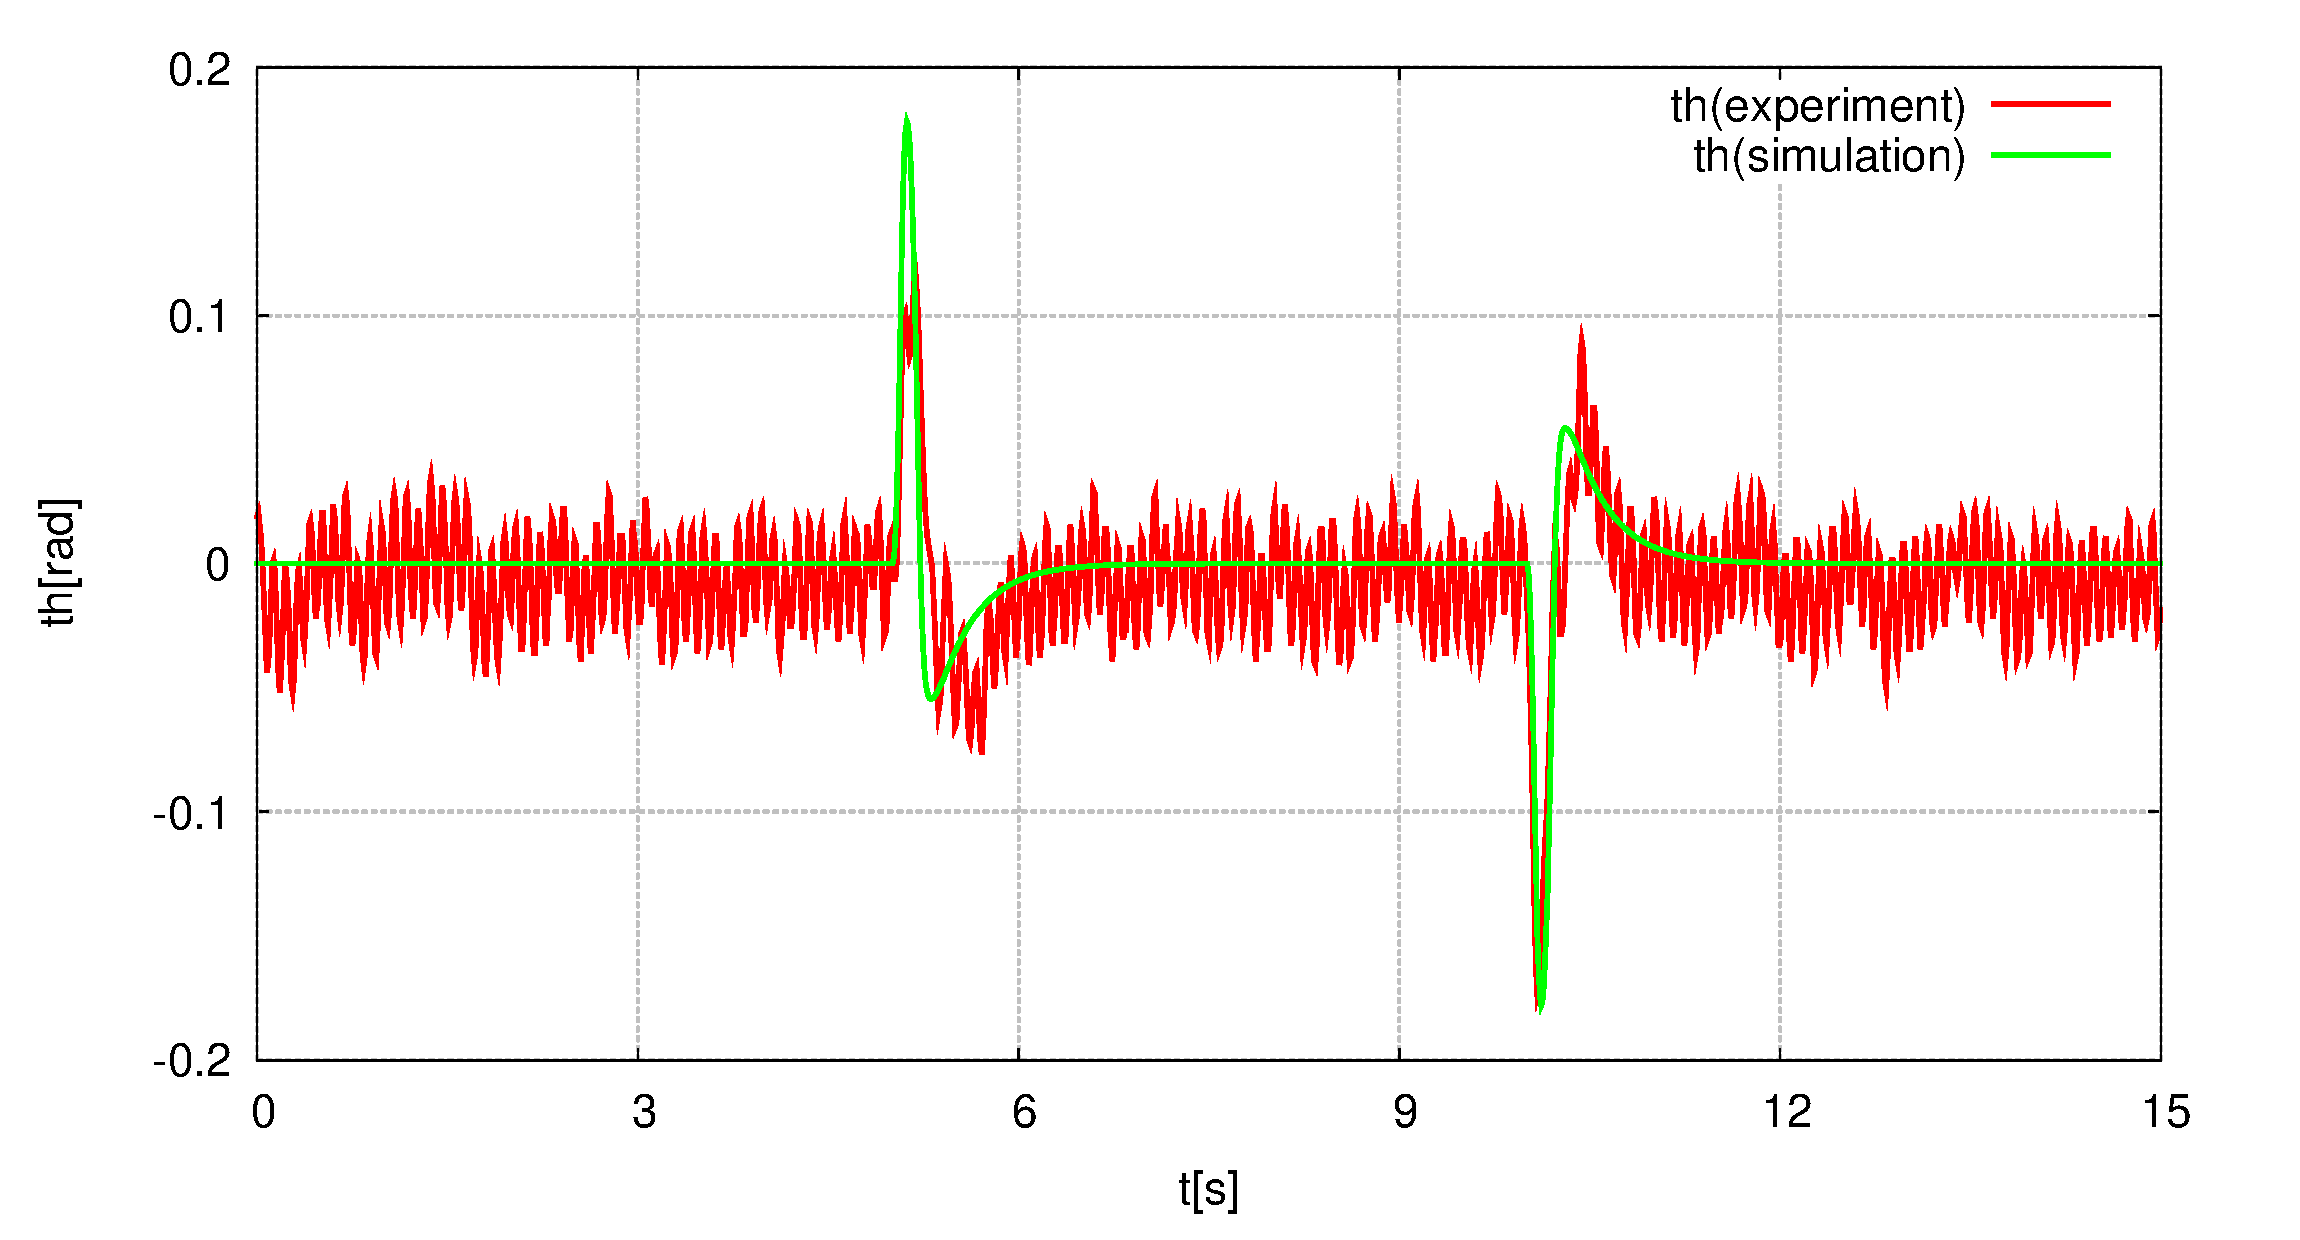
\includegraphics[width=0.49\linewidth]{gazo/experiment_Q65obs30dt10TH2.eps}
		\caption{比較結果その9(左図がr,右図が$\theta$)}
		\label{image:sono9}
	\end{figure}
	\begin{figure}[H]
		\centering
		\includegraphics[width=0.49\linewidth]{gazo/experiment_Q55obs60dt10R2.eps}
		\includegraphics[width=0.49\linewidth]{gazo/experiment_Q55obs60dt10TH2.eps}
		\caption{比較結果その10(左図がr,右図が$\theta$)}
		\label{image:sono10}
	\end{figure}
	\begin{figure}[H]
		\centering
		\includegraphics[width=0.49\linewidth]{gazo/experiment_Q56obs60dt10R2.eps}
		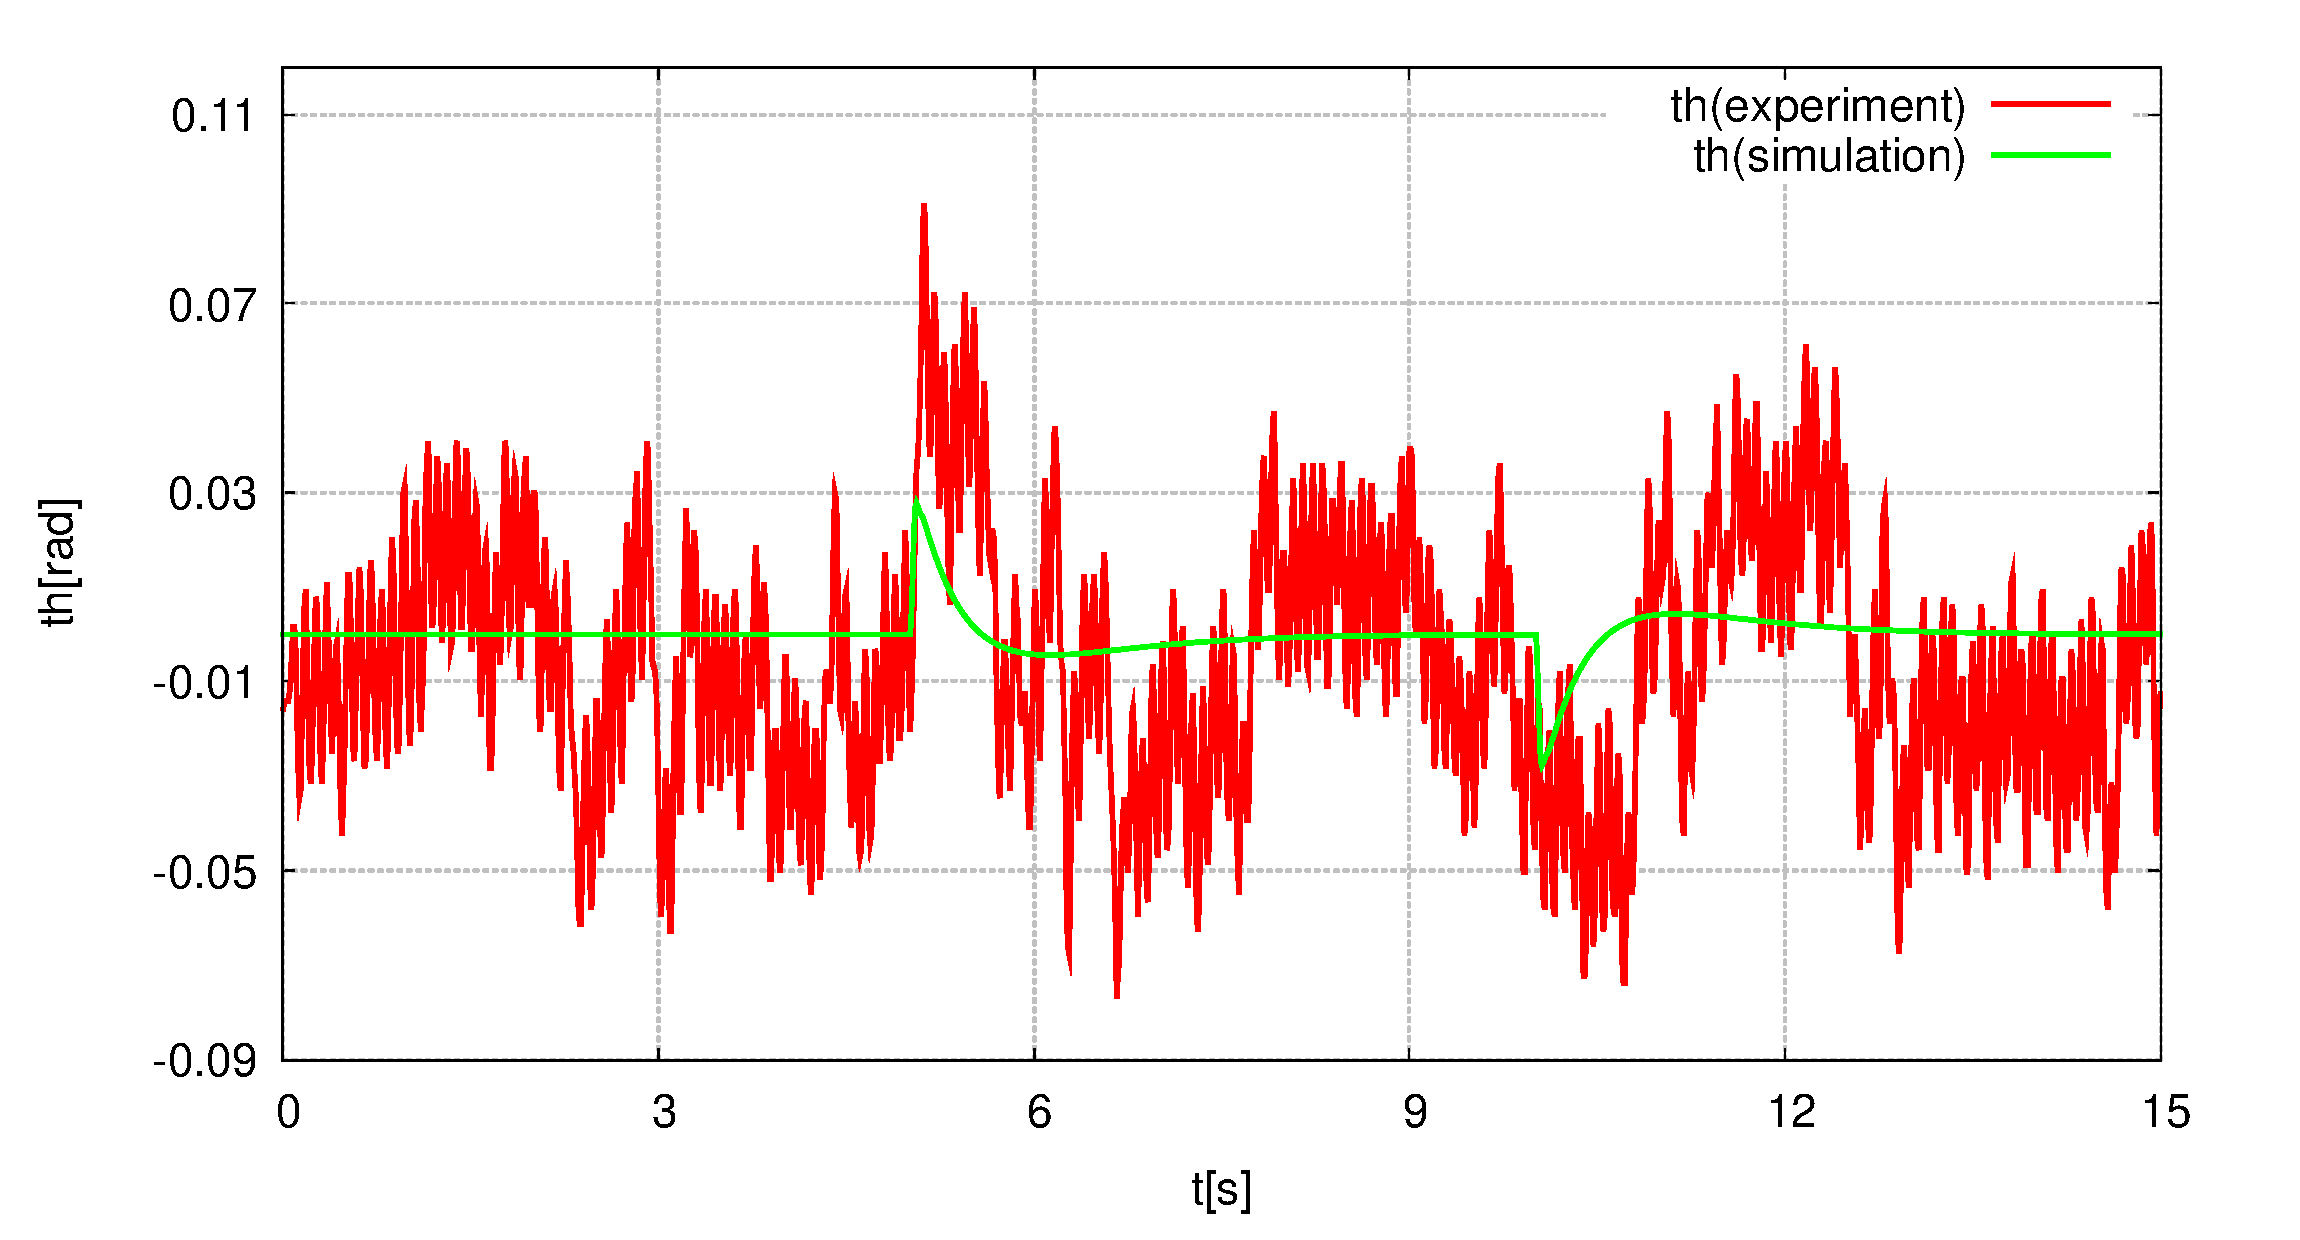
\includegraphics[width=0.49\linewidth]{gazo/experiment_Q56obs60dt10TH2.eps}
		\caption{比較結果その11(左図がr,右図が$\theta$)}
		\label{image:sono11}
	\end{figure}
	\begin{figure}[H]
		\centering
		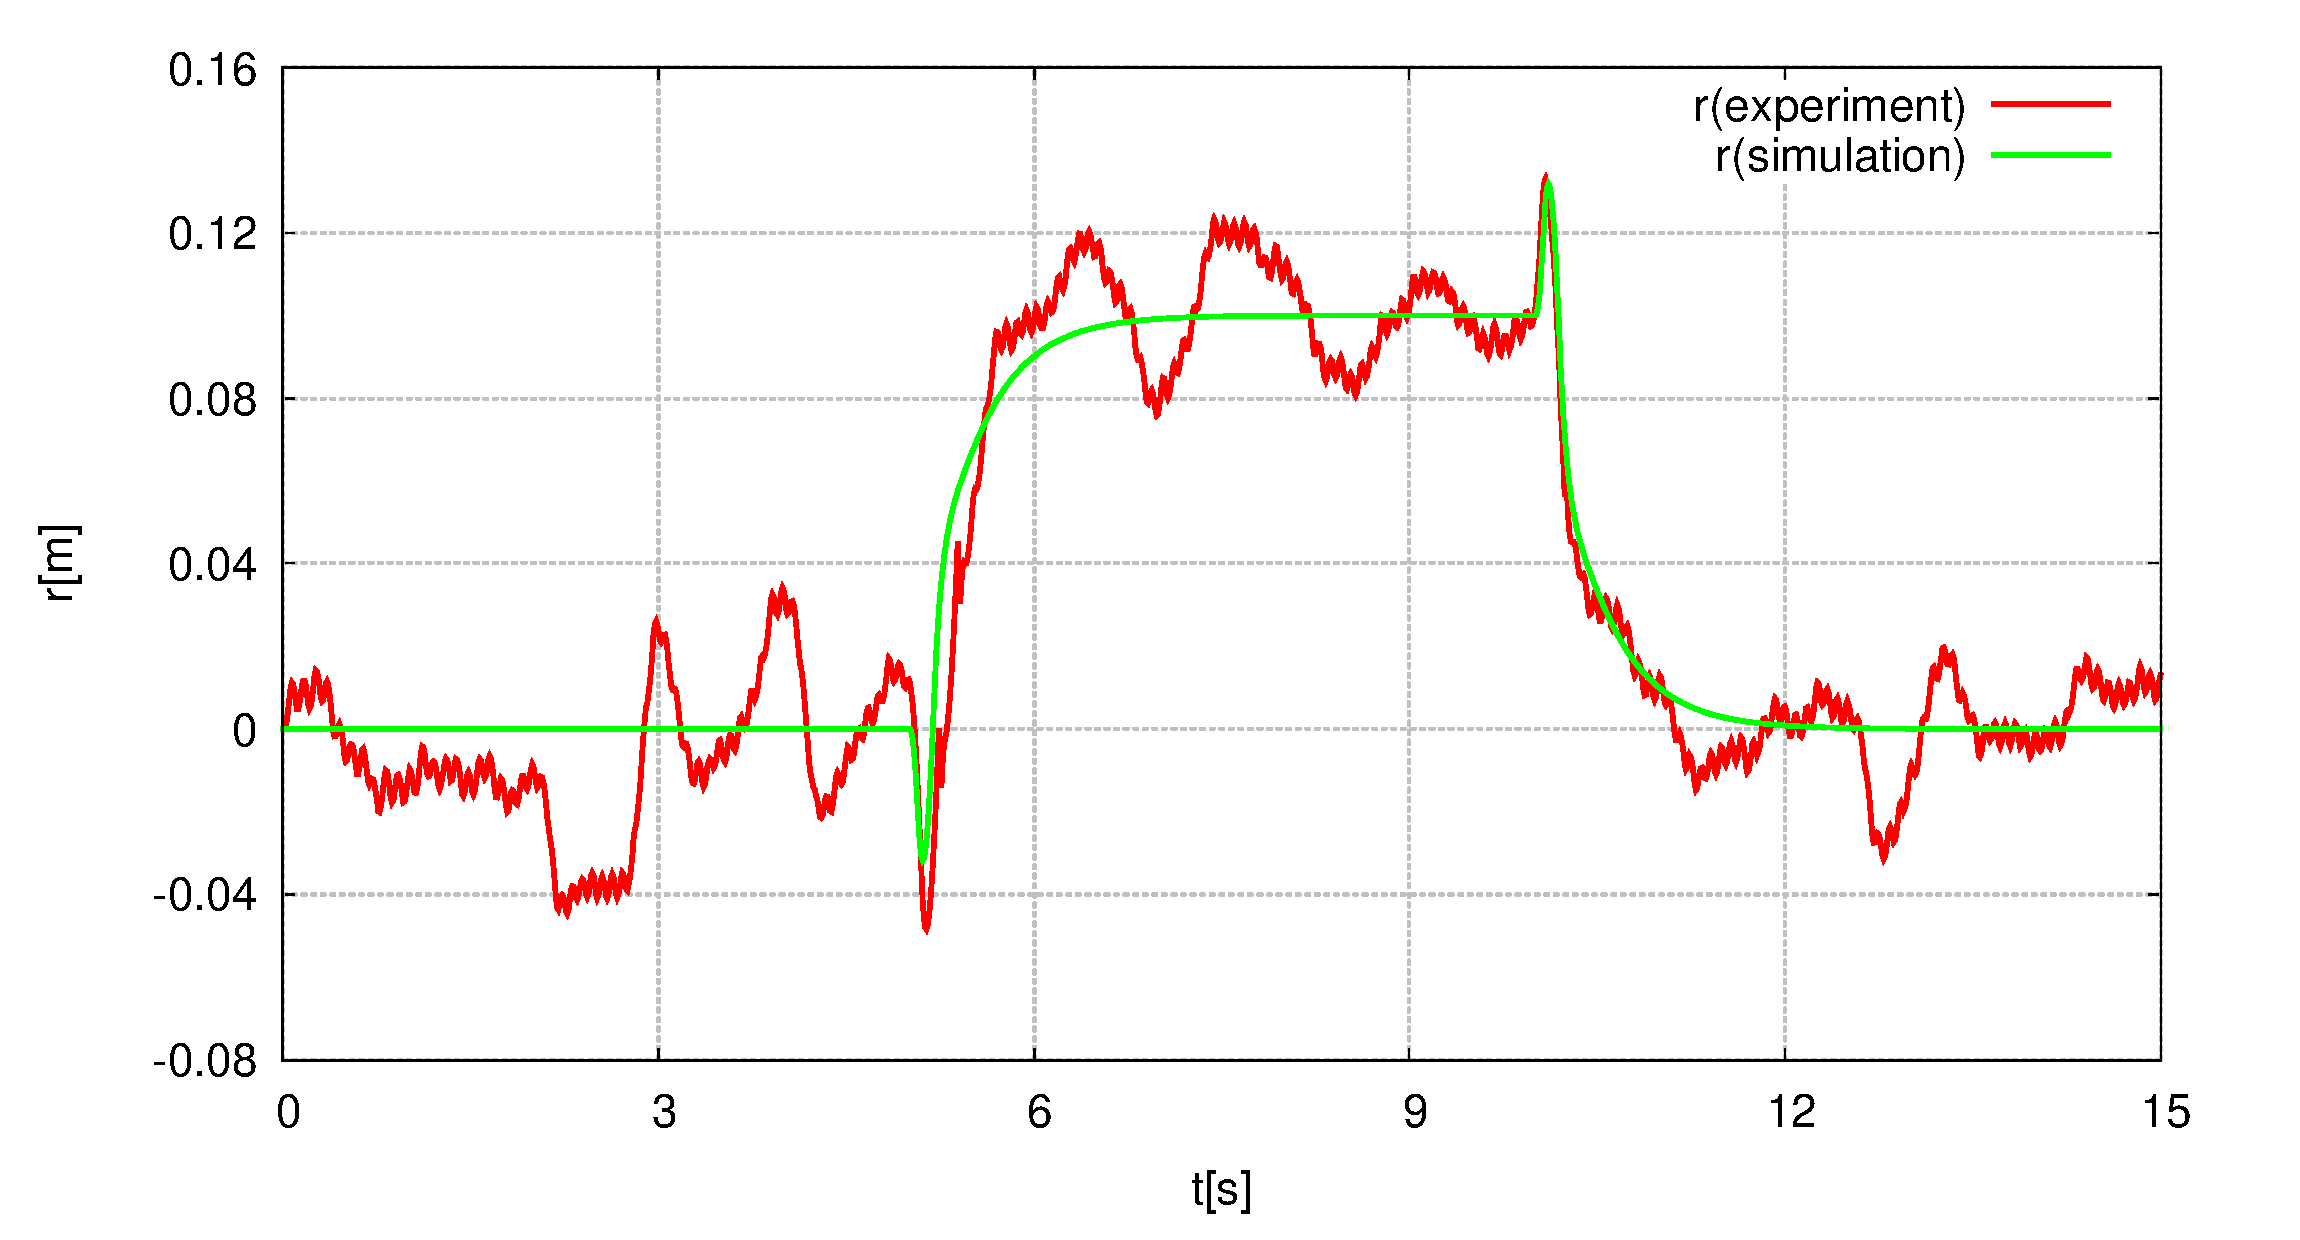
\includegraphics[width=0.49\linewidth]{gazo/experiment_Q65obs60dt10R2.eps}
		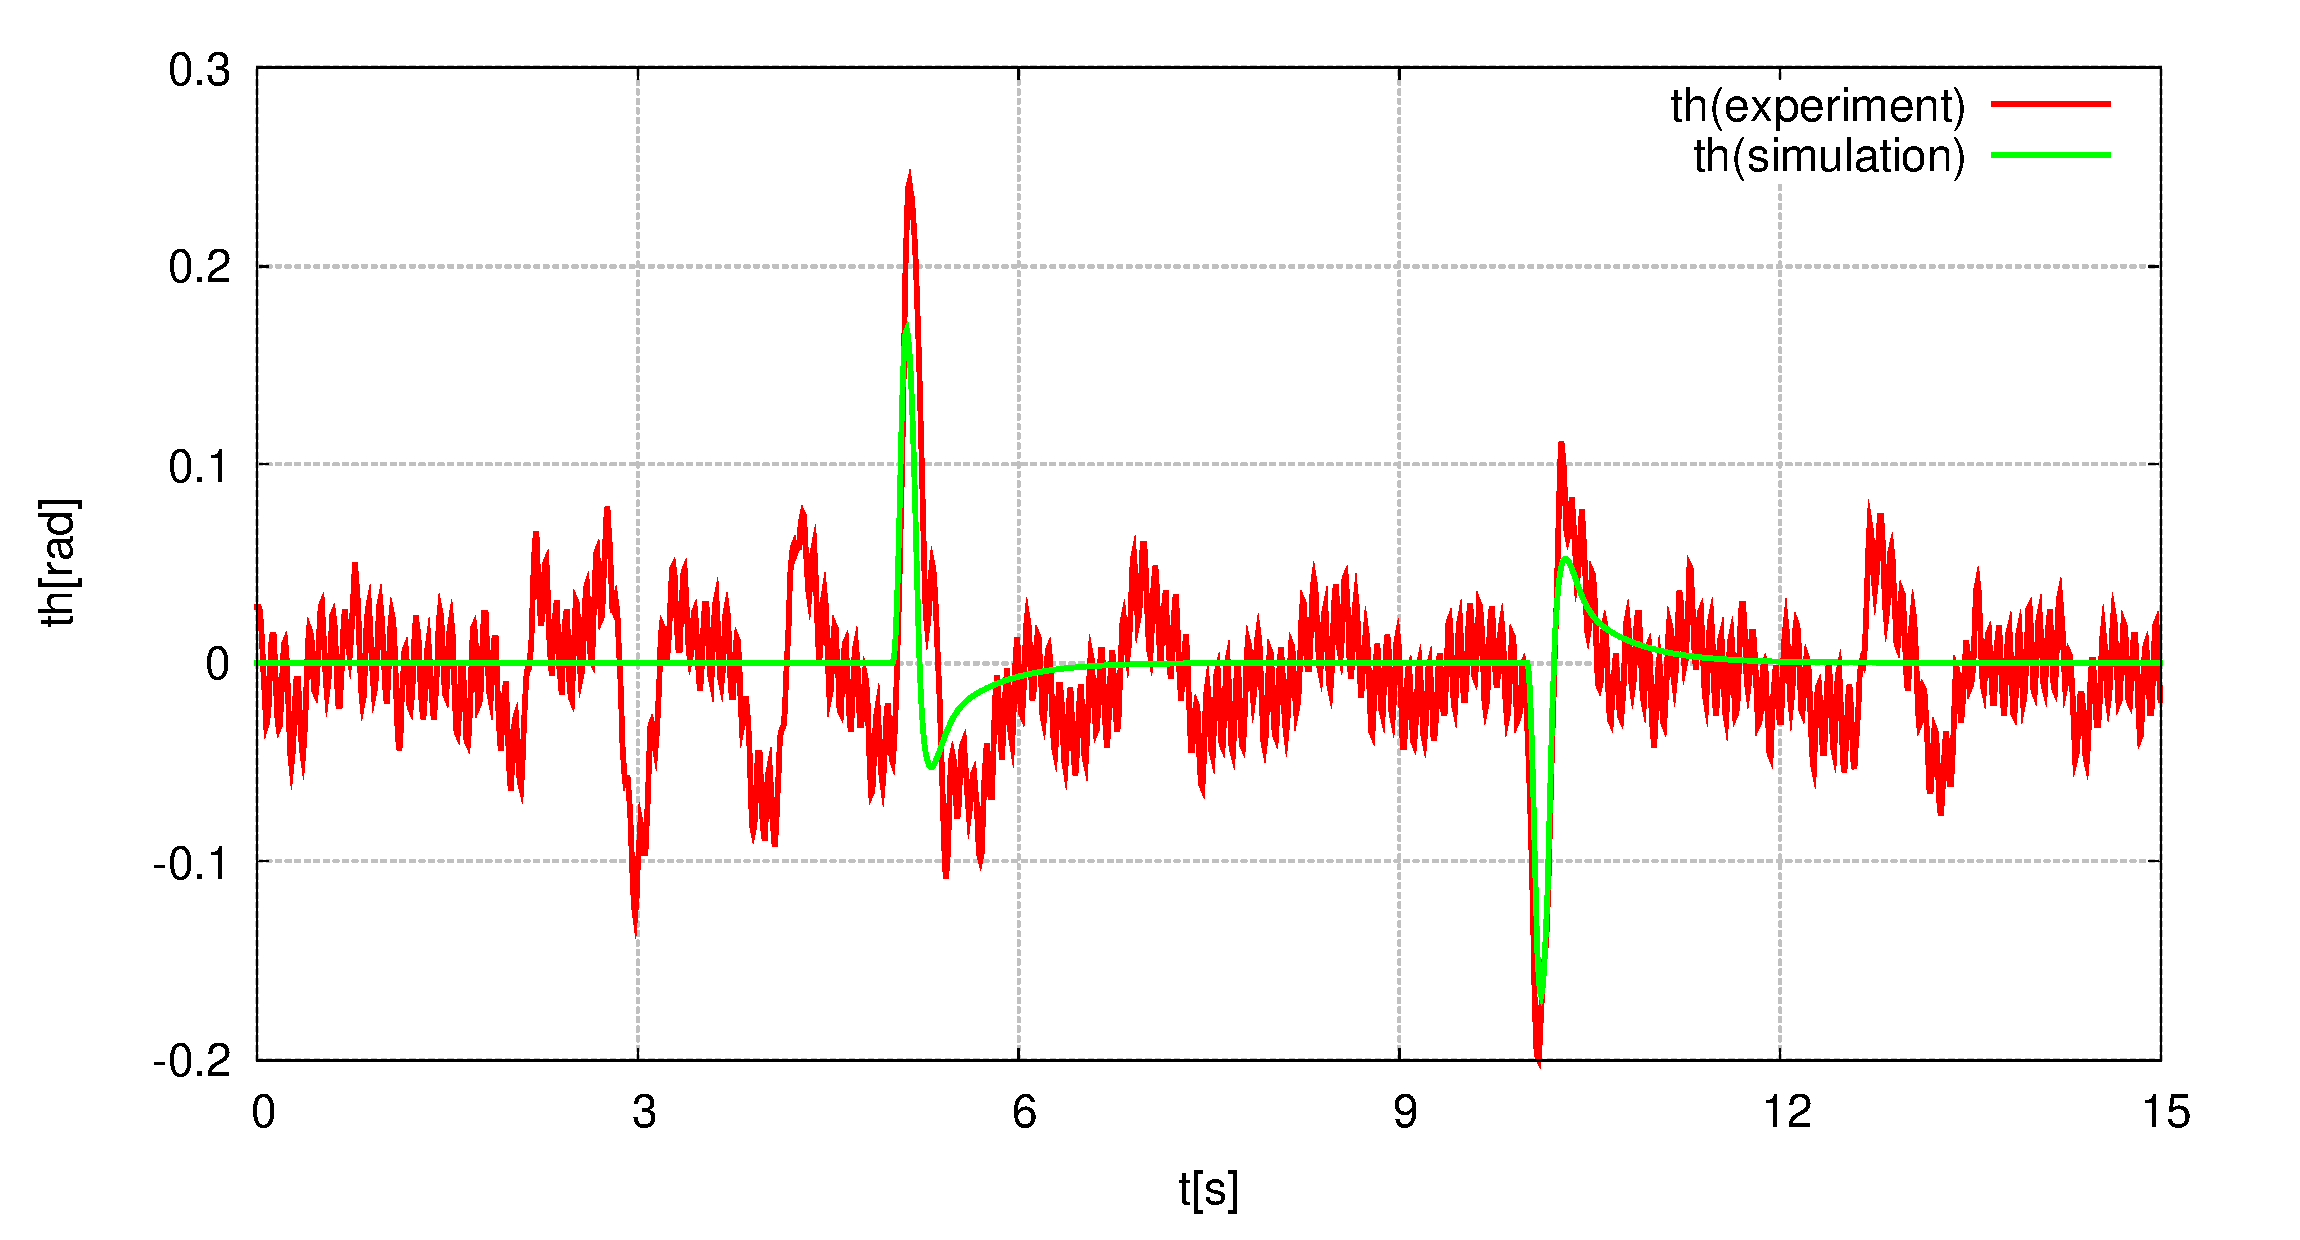
\includegraphics[width=0.49\linewidth]{gazo/experiment_Q65obs60dt10TH2.eps}
		\caption{比較結果その12(左図がr,右図が$\theta$)}
		\label{image:sono12}
	\end{figure}
	以上の図を見てみるとすべての図においてノイズがひどいが、比較的シミュレーション結果とほぼ一致している図とほとんど一致していない図があるのが分かる。
	前者に当てはまる図は図\ref{image:sono1}、図\ref{image:sono3}、図\ref{image:sono4}、図\ref{image:sono6}
	、図\ref{image:sono7}、図\ref{image:sono9}、図\ref{image:sono12}。後者に当てはまる図は、
	図\ref{image:sono2}、図\ref{image:sono5}、図\ref{image:sono8}、図\ref{image:sono11}である。
	後者に共通する特徴は重み行列が$\rm{diag}(1E5,1E6,1,1)$となっている点である。
	このようにしたときの特徴としてはシミュレーションの章でも述べたが、大きくした成分に対応する状態の応答がよくなるというものであった。
	つまり、この重み行列のとき$\theta$の応答がよくなりるはずである。
	だが、実際の図を見てみると$\theta$の応答はシミュレーションと比較しても一致しているとは言えない。
	また、$r$に関しては図を見る限りでは目標値変更に追従できていないといえる。
	これは、重み行列をこのようにしたことで状態のバランスが崩れ、$r$の応答が遅くなったためといえる。
	普通であれば、プログラムが5秒おきに目標値を変更するので、台車はその目標値に向かって動き出す。
	しかし、$r$の応答が遅いため台車は目標値に到達することができずに、プログラムから次の目標値が入力される。
	こうなってしまうことで台車は常に動き続けている状態になり、応答が良くなるはずの$\theta$もそれに伴い
	悪くなるといえる。そのため、$r$は目標値に追従できず、$\theta$の応答も悪くなってしまったといえる。
	\par
	シミュレーションと実験において差異がでたが目標値変更を行っての安定化制御を行うことができたので
	実験目的の第二項目は達成できたといえる。
	
	

%-----------------------------------------------------------
\newpage
\section{振り上げ制御及び安定化実験}
	振子を真下に配置し、そこから台車の動きだけで振子を振り上げ、
	安定化制御が可能か実験を行う(実験項目の第三項目)。
	以下に$k$を変更したときの実験結果を示す。
	\begin{figure}[H]
		\centering
		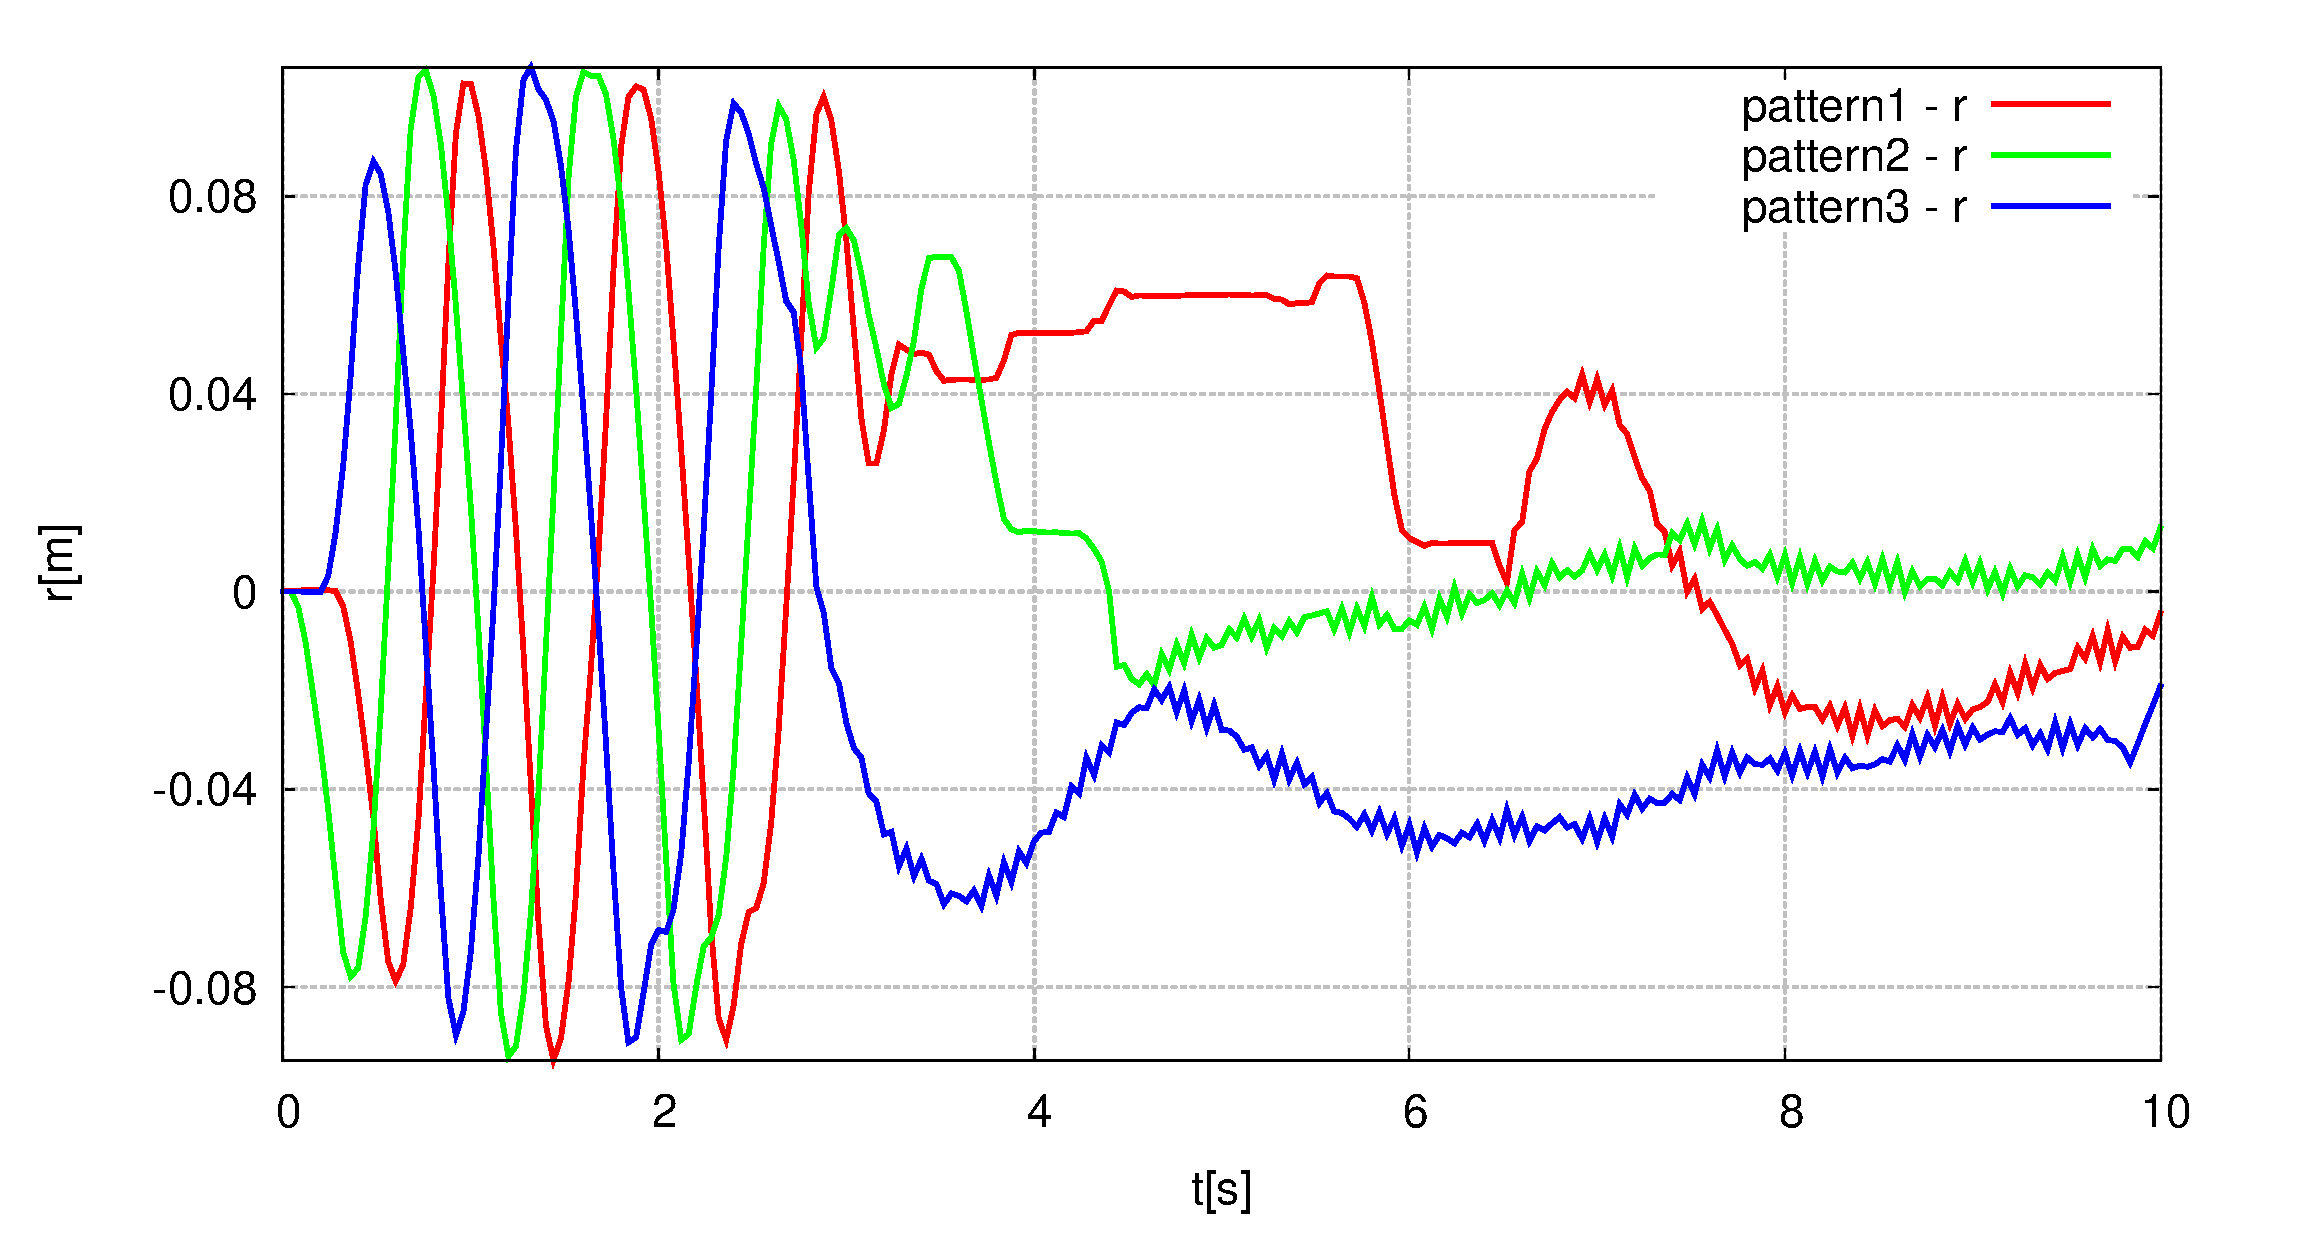
\includegraphics[width=0.49\linewidth]{gazo/Hexpe_R.eps}
		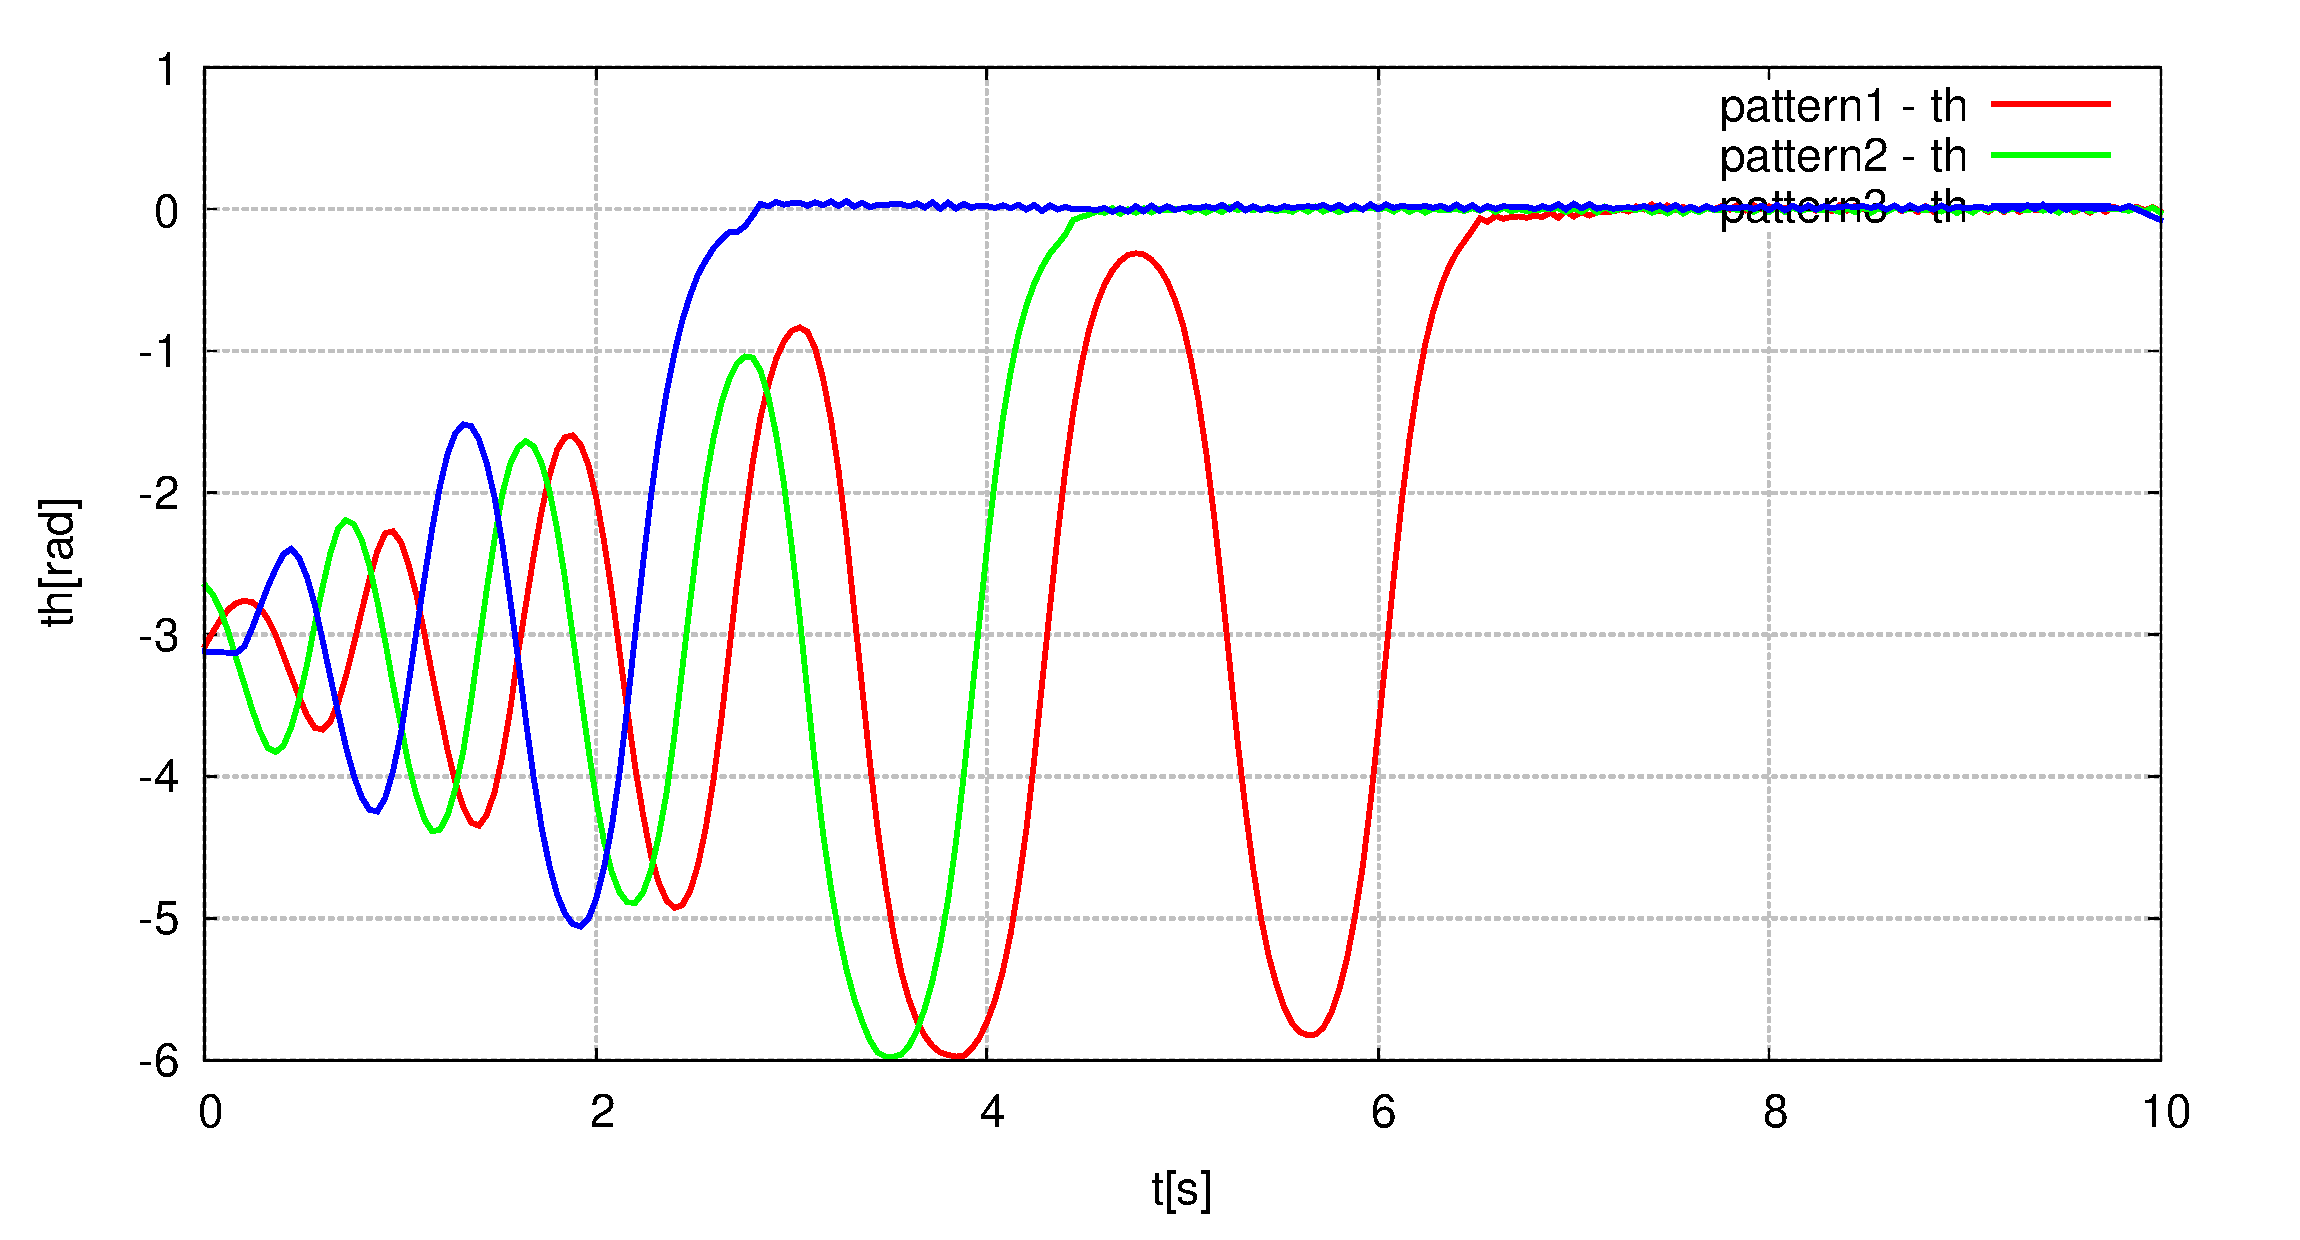
\includegraphics[width=0.49\linewidth]{gazo/Hexpe_TH.eps}
		\caption{$k$の違いによる実験結果の比較}
		\label{image:Hexpe}
	\end{figure}
	図中のPatternは以下の表に対応するパラメータである。
	\begin{table}[H]
		\begin{center}
			\caption{実験に用いたパラメータの組}
			\medskip
			
			\begin{tabular}{|c|c|c|}\hline
				& $n$ & $k$ \\ \hline\hline
				パターン1 & 0.4 & $1.0×10^3$  \\ \hline
				パターン2 & 0.4 & $1.0×10^4$  \\ \hline
				パターン3 & 0.4 & $1.0×10^5$  \\ \hline
			\end{tabular}
		\end{center}
		\label{table:huriage_huriage}
	\end{table}
	図\ref{image:Hexpe}の右図より、$k$の値が大きいほど早く安定化制御に移行していることがわかる。
	$k$が大きくなるとエネルギーの収束が早くなるため、より早く安定化制御に移行できたといえる。
	左図においても3パターンとも違う挙動を示していることがわかる。
	つまり、シミュレーションと実験では違う結果が確認されたことになる。これは、シミュレーションで用いたモデルにおいて、
	実際の倒立振子に存在する考慮すべき点を考慮していなかった可能性があるのではないかと考える。
	\par
	実験において倒立振子は机に置かれているだけと第一章で述べた。これにより台車の動きによって倒立振子自体が机の上で動くことが確認された。
	ここで確認された事象はシミュレーションでは考慮されていない点の一つであるが、ここに述べていない点についても
	考慮すべき点が存在すると考えられる。今回の目的はシミュレーションと実験結果を一致させることではないためこれ以上の言及は避けておく。
	\par
	以下に実験結果とシミュレーション結果との比較を行った図を示す。
	\begin{figure}[H]
		\centering
		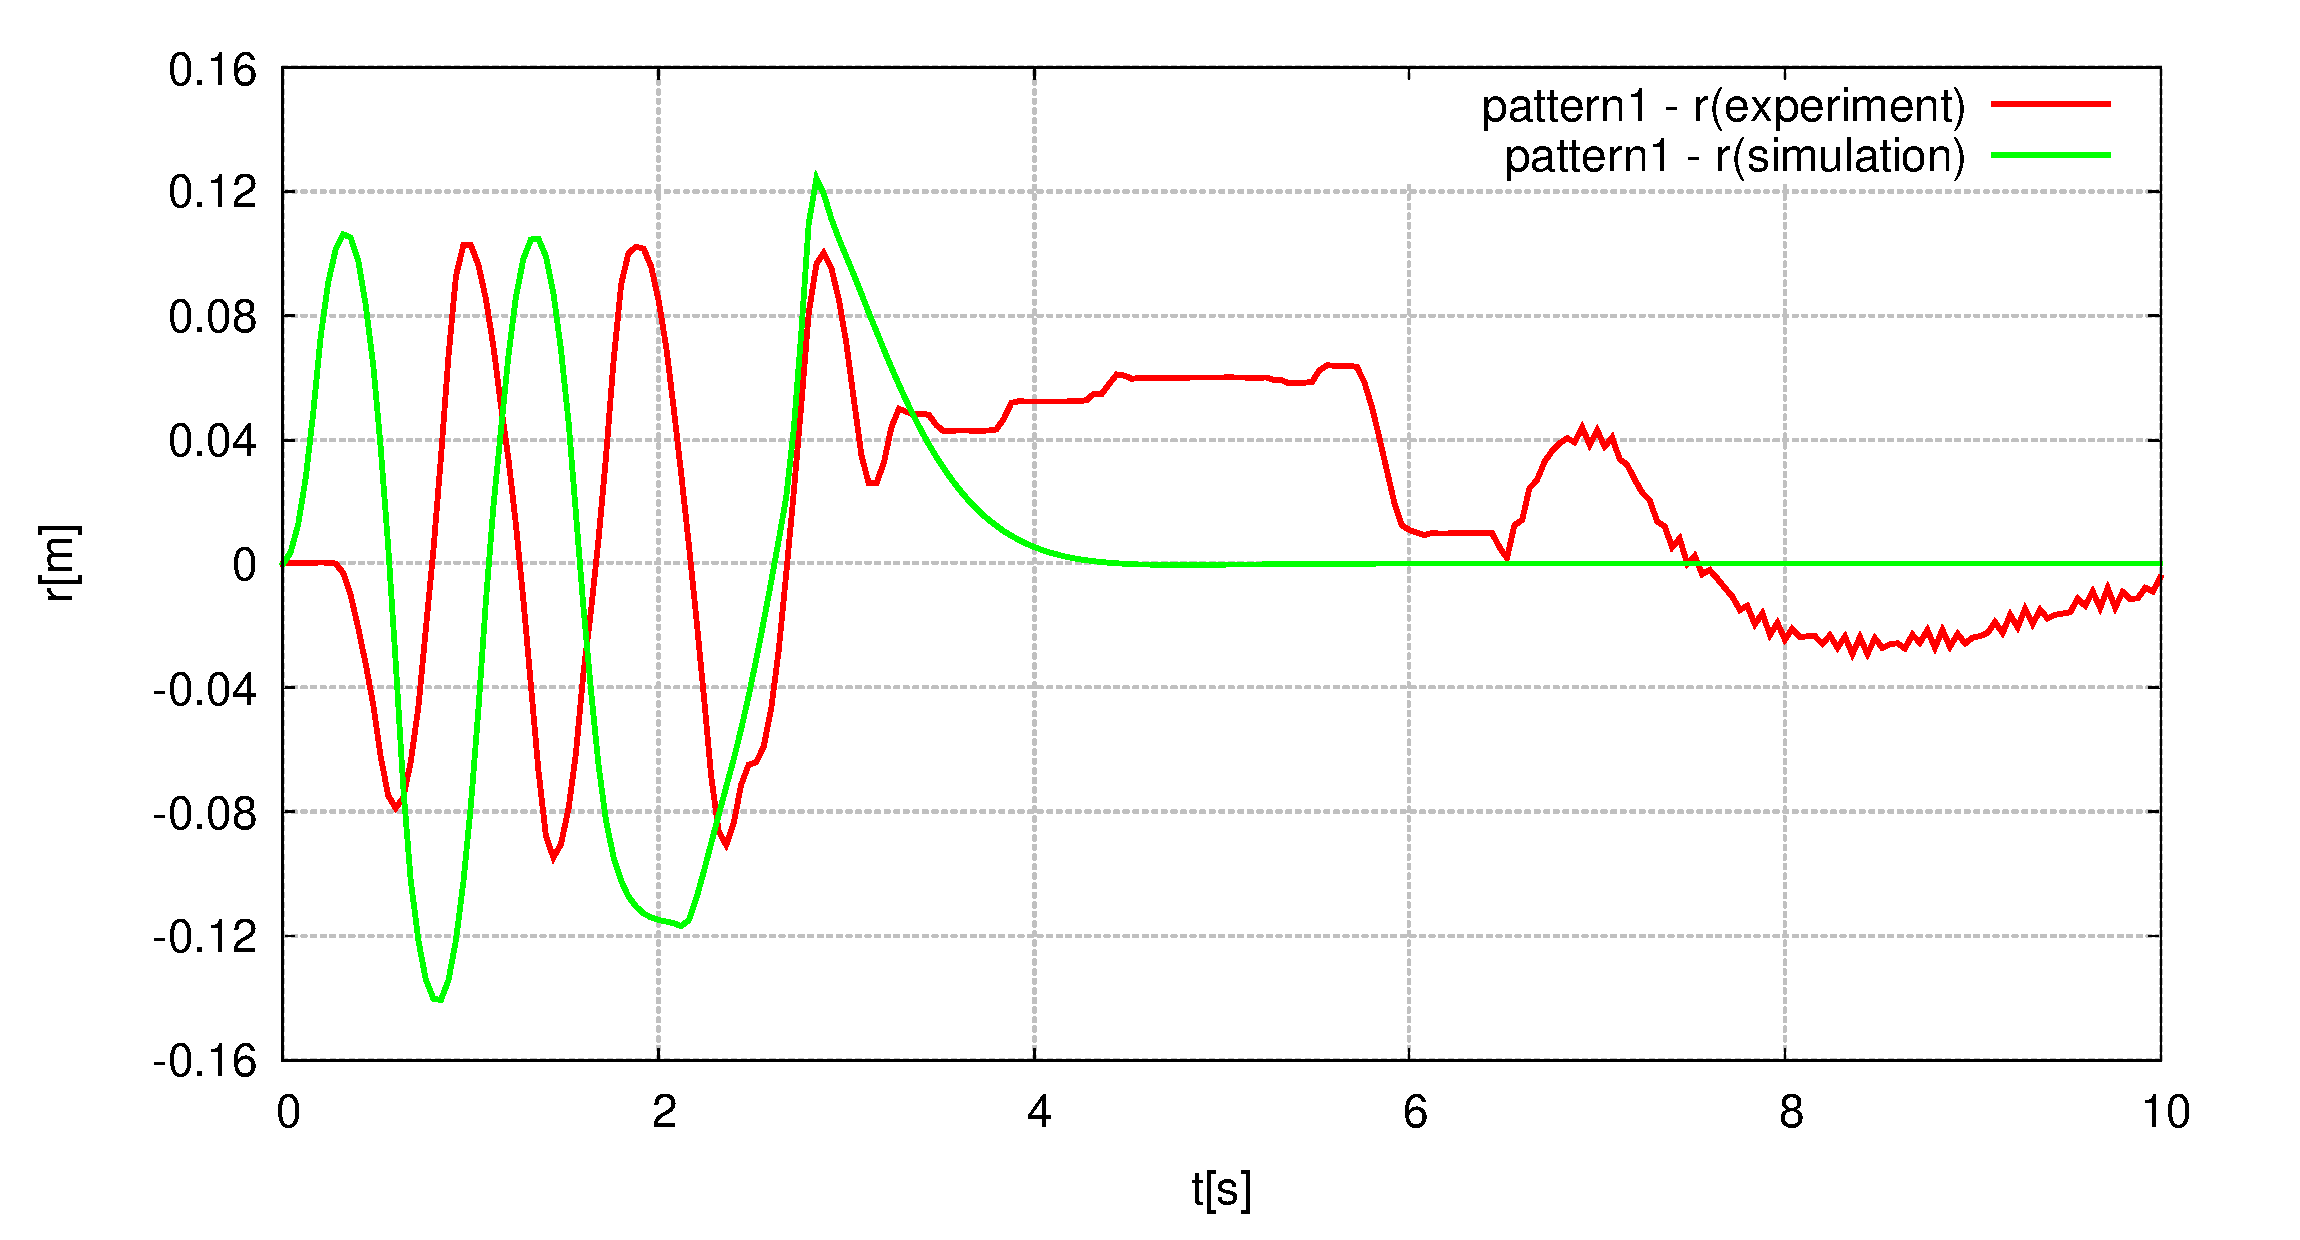
\includegraphics[width=0.49\linewidth]{gazo/HcompP1R.eps}
		\includegraphics[width=0.49\linewidth]{gazo/HcompP1TH.eps}
		\caption{比較結果(Pattern1)}
		\label{image:HcompP1}
	\end{figure}
	\begin{figure}[H]
		\centering
		\includegraphics[width=0.49\linewidth]{gazo/HcompP2R.eps}
		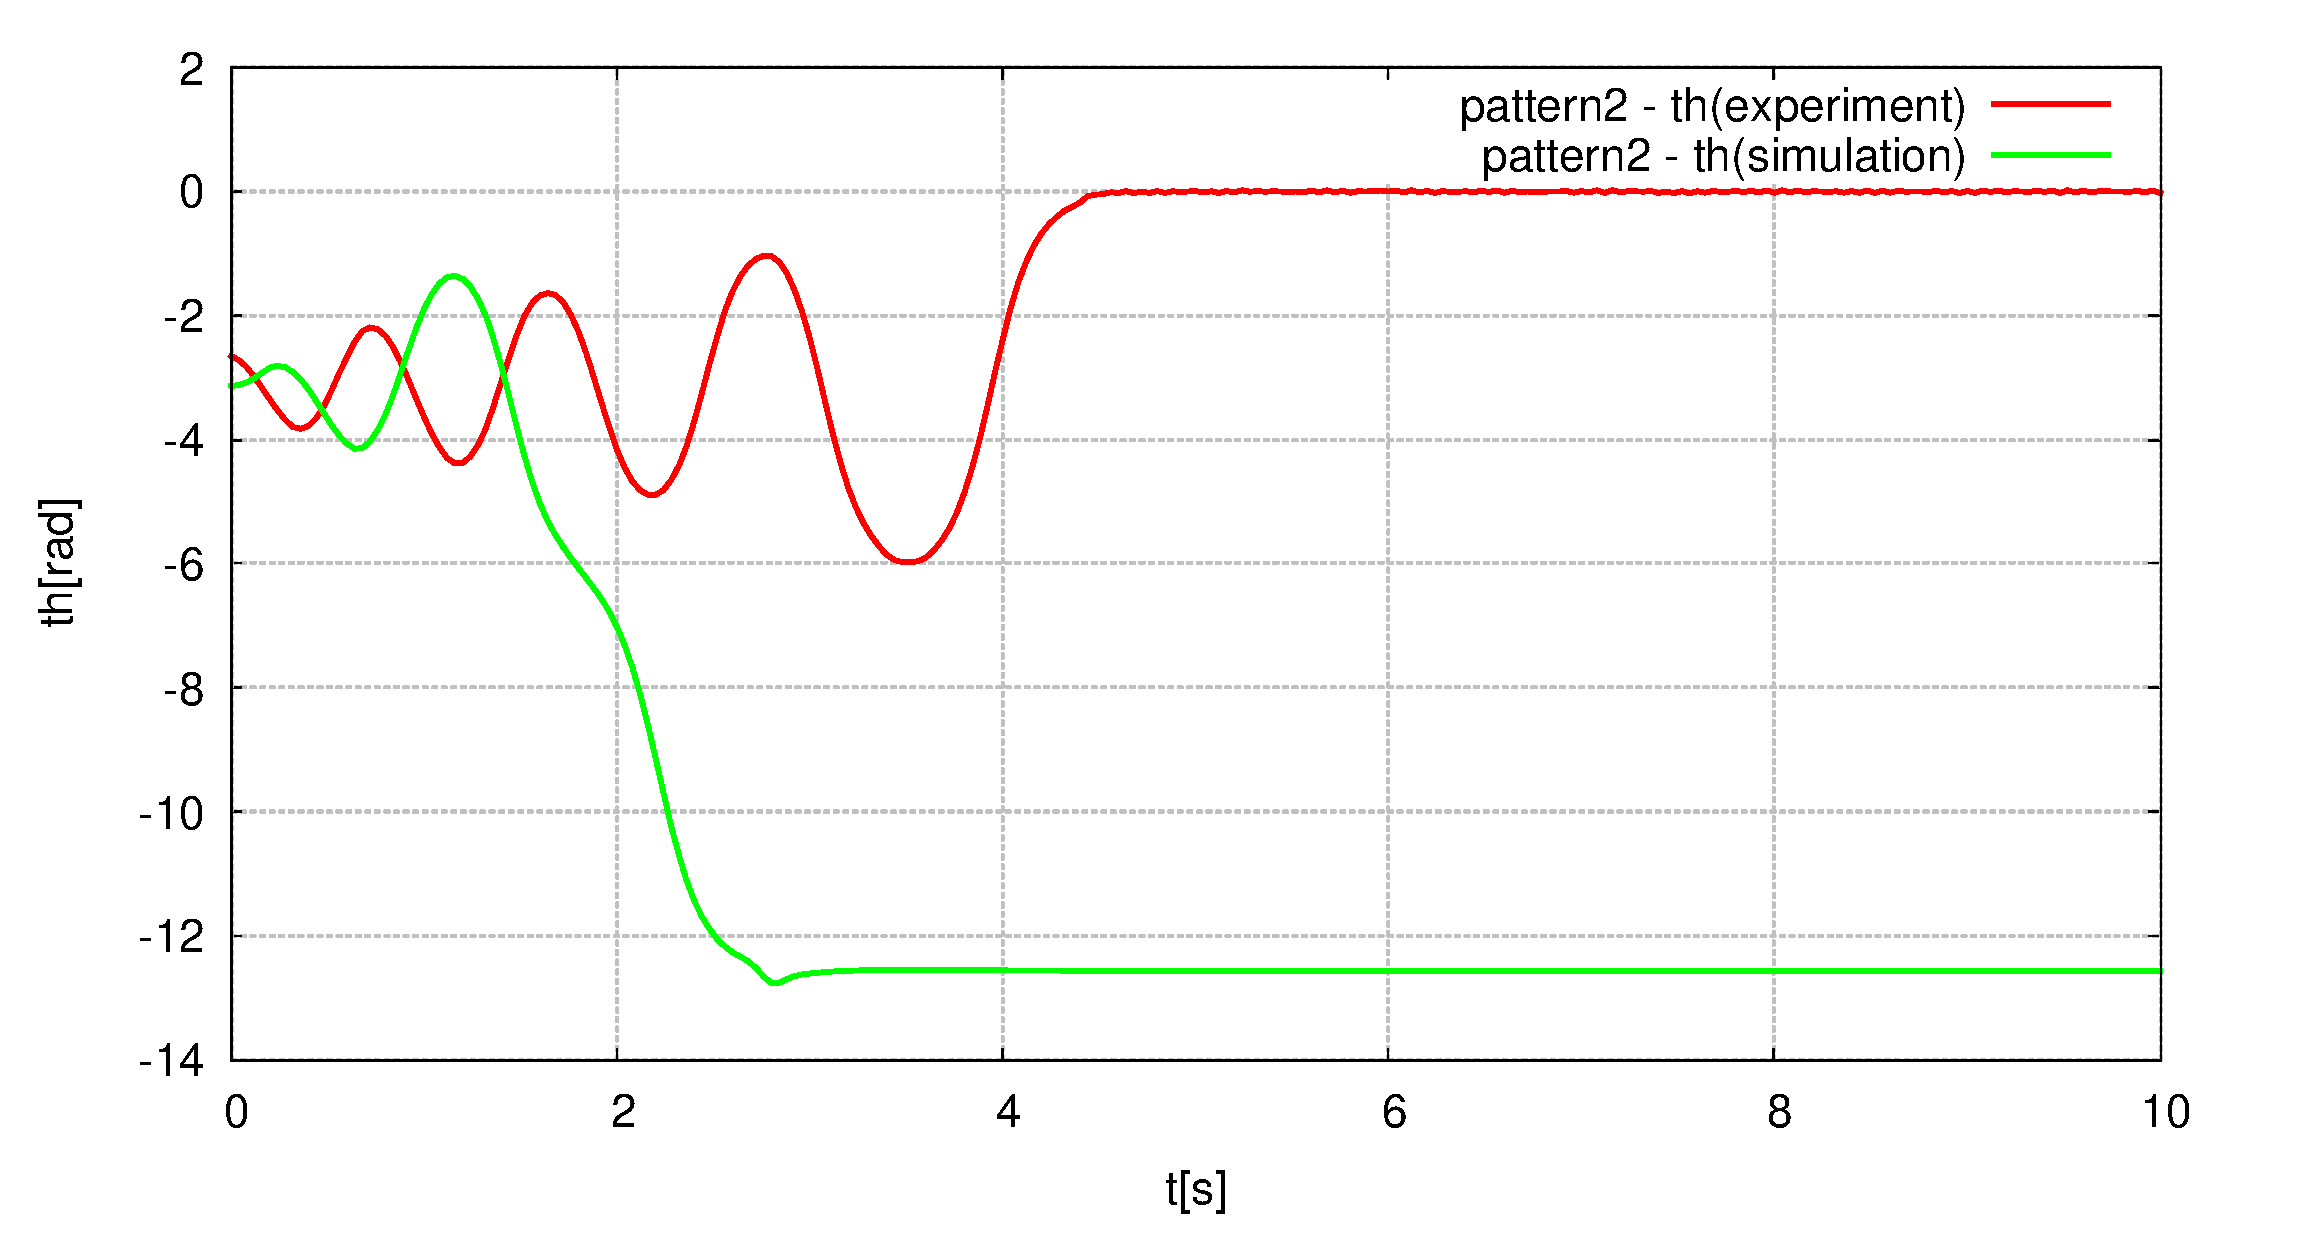
\includegraphics[width=0.49\linewidth]{gazo/HcompP2TH.eps}
		\caption{比較結果(Pattern2)}
		\label{image:HcompP2}
	\end{figure}
	\begin{figure}[H]
		\centering
		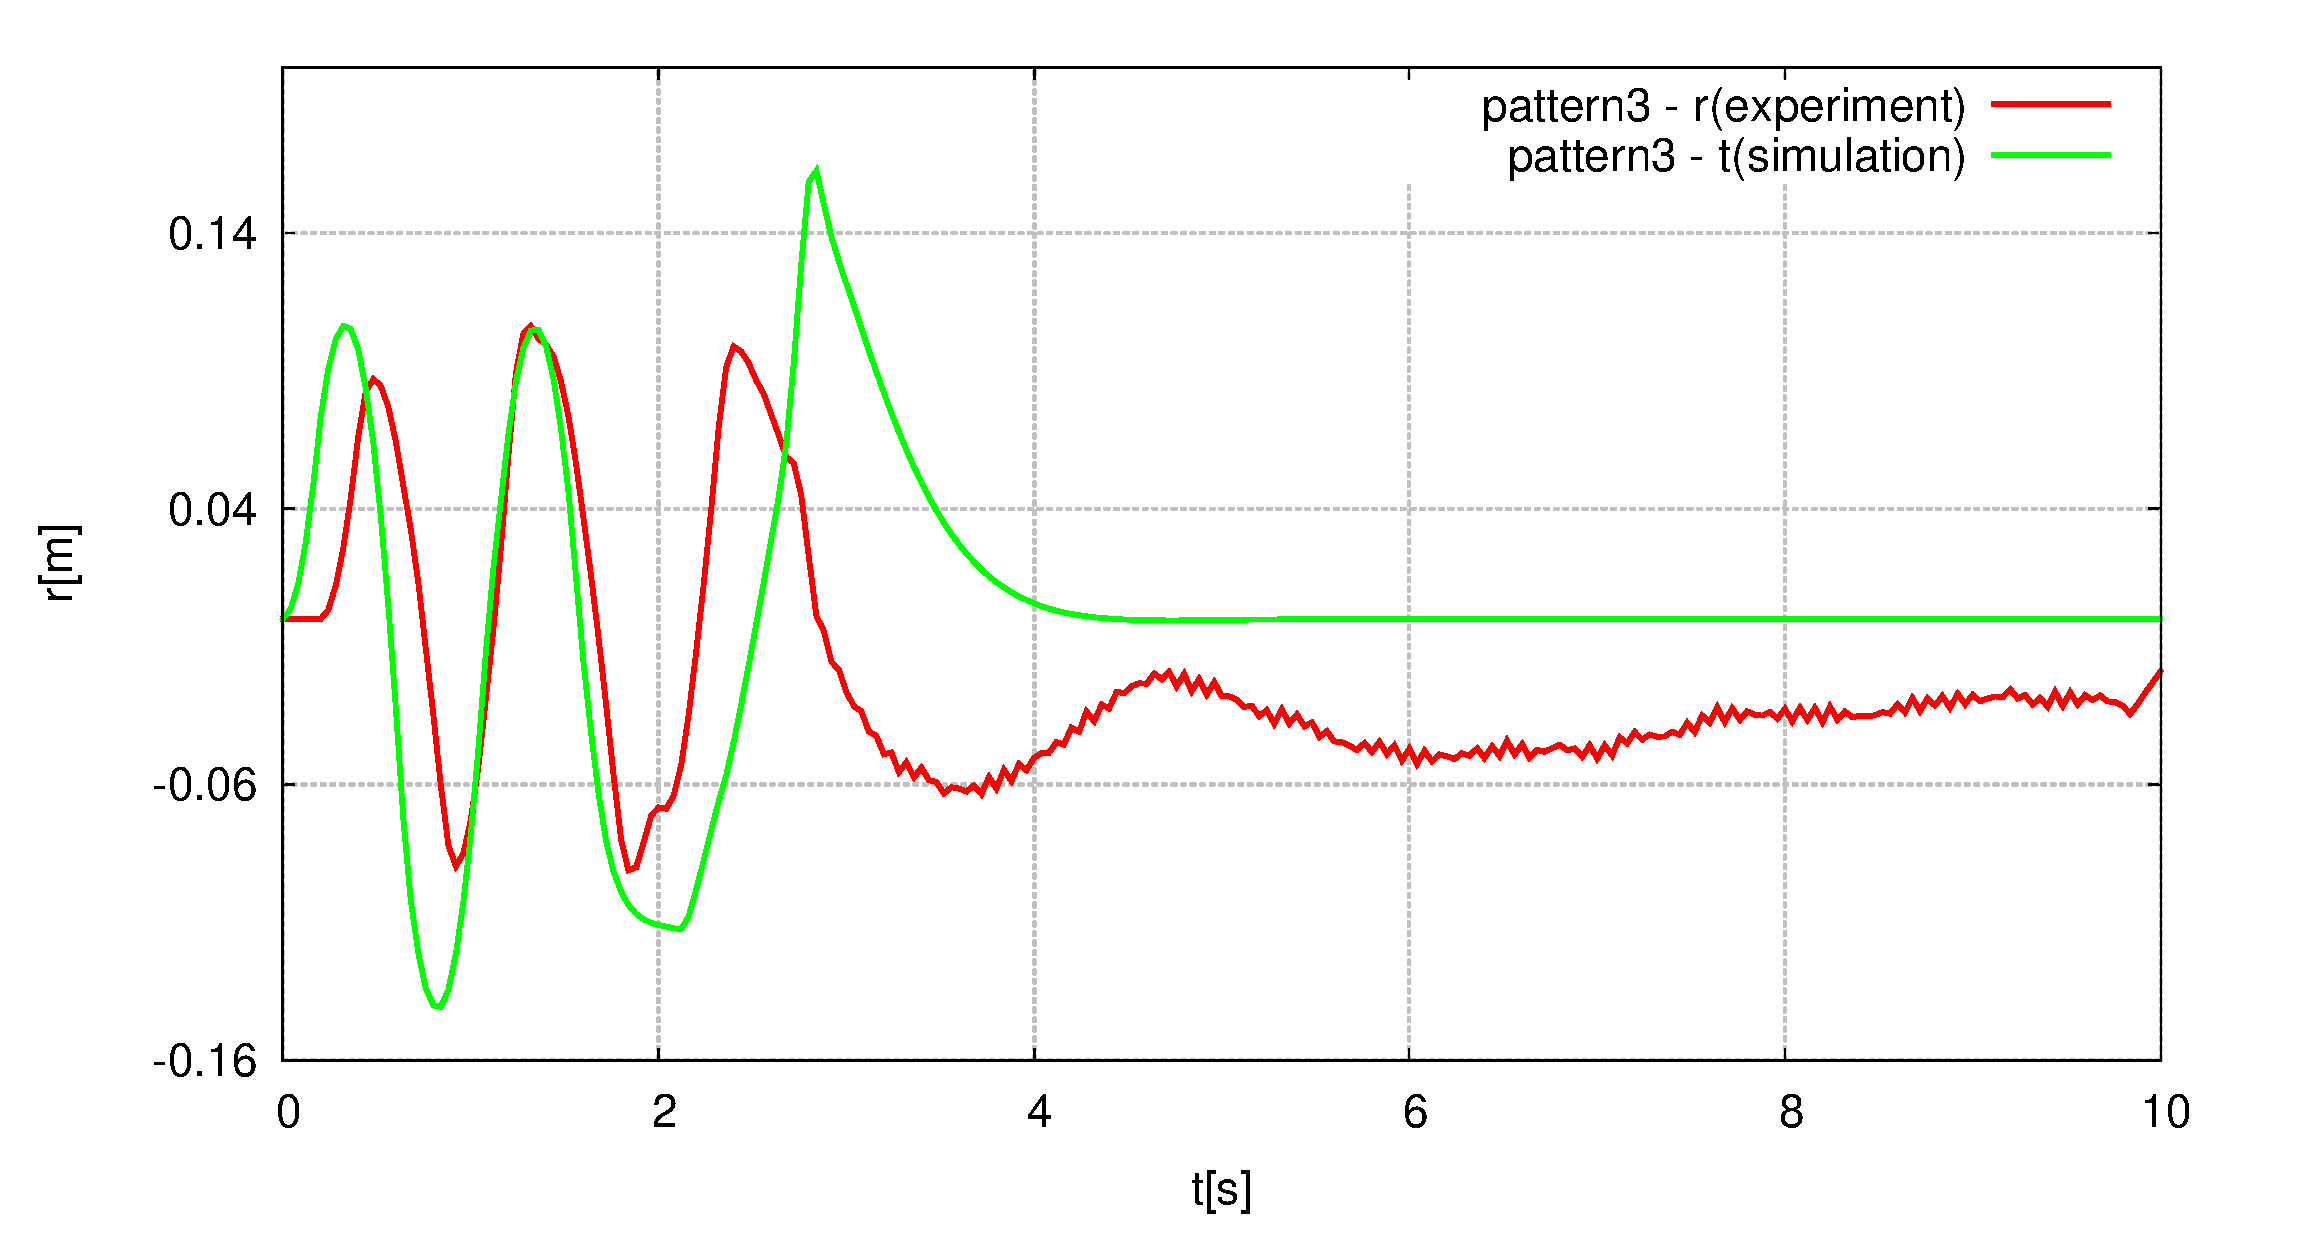
\includegraphics[width=0.49\linewidth]{gazo/HcompP3R.eps}
		\includegraphics[width=0.49\linewidth]{gazo/HcompP3TH.eps}
		\caption{比較結果(Pattern3)}
		\label{image:HcompP3}
	\end{figure}
	
	\par
	先ほども述べたように図\ref{image:HcompP1}、図\ref{image:HcompP2}、図\ref{image:HcompP3}からシミュレーションと実験の結果が一致していないことが確認できる。
	しかし、図\ref{image:HcompP3}の右図においては、収束角度が違うだけで、収束までにかかった時間やその挙動はほとんど同じといえる。だが、左図についてはシミュレーションと
	実験では台車の挙動に差異がみられる。この台車の動きの差異から振り子の収束角度が違ってしまったのではないかと考えられる。
	\par
	シミュレーションの結果と実験の結果に大きな違いが出てしまったが、実験において振り上げ制御から安定化制御を行うことができたので、実験目的の第三項目を達成できたといえる。
	
%-----------------------------------------------------------